% =============================================================================
% Revitalization in Shrinking Cities: Impact of the Neighborhood
% Stabilization Program in Detroit
% Authors: Camila Alvayay Torrejon & Mark Skidmore
% Target: Journal of Housing Economics
% =============================================================================

\documentclass[12pt,authoryear]{elsarticle}

% ---- Packages ----
\usepackage[utf8]{inputenc}
\usepackage[T1]{fontenc}
\usepackage{amsmath,amssymb}
\usepackage{graphicx}
\usepackage{booktabs}
\usepackage{multirow}
\usepackage{tabularx}
\usepackage{threeparttable}
\usepackage{siunitx}
\usepackage{float}
\usepackage{setspace}
\usepackage[margin=1in]{geometry}
\usepackage{hyperref}
\usepackage{natbib}
\usepackage{caption}
\usepackage{subcaption}
\usepackage{pdflscape}
\usepackage{rotating}
\usepackage{appendix}
\usepackage{longtable}
\usepackage{lmodern}

% ---- Path for figures ----
\graphicspath{{figures/}}

% ---- Bibliography style ----
\bibliographystyle{elsarticle-harv}

% ---- Document ----
\begin{document}

\begin{frontmatter}

\title{Revitalization in Shrinking Cities: Impact of the Neighborhood Stabilization Program in Detroit}

\author[ucn]{Camila Alvayay Torrej\'on\corref{cor1}}
\ead{alvayayt@ucn.cl}
\author[msu]{Mark Skidmore}
\ead{mskidmor@msu.edu}

\cortext[cor1]{Corresponding author.}

\affiliation[ucn]{organization={Department of Economics, Universidad Cat\'olica del Norte},
            city={Antofagasta},
            country={Chile}}
\affiliation[msu]{organization={Department of Agricultural, Food, and Resource Economics, Michigan State University; Lincoln Institute of Land Policy},
            city={East Lansing, MI},
            country={United States}}

\begin{abstract}
The Great Recession resulted in a significant collapse in the United States housing market, with foreclosure rates soaring in cities experiencing long-term economic decline. Detroit, which had the second-highest foreclosure rate among the nation's 100 largest metropolitan areas by the end of 2007, received approximately \$70 million through the Neighborhood Stabilization Program (NSP)---a federal place-based policy targeting the most distressed neighborhoods. This paper evaluates the impact of NSP on housing prices and foreclosure rates in Detroit using the \citet{callaway2021} difference-in-differences estimator, which exploits the staggered treatment timing of NSP1 (2009) and NSP3 (2011). We address the selection problem by including HUD formula variables and demographic characteristics in the propensity score. Once these controls are included, the overall effects are small and statistically insignificant for housing prices (ATT $= -0.017$, $p = 0.740$) and marginally significant for foreclosure rates (ATT $= +0.094$, $p = 0.058$). However, cohort-specific estimates reveal striking heterogeneity: NSP1 areas show null price effects and borderline increases in foreclosures, while NSP3 areas show a significant 21.7\% increase in sale prices ($p = 0.014$). Dropping adjacent control block groups to address potential spillover effects strengthens the foreclosure result ($p = 0.020$). These findings suggest that the program's effectiveness depended critically on the timing of implementation relative to the crisis cycle, with later rounds benefiting from stabilizing market conditions.
\end{abstract}

\begin{keyword}
Neighborhood Stabilization Program \sep Detroit \sep housing market \sep difference-in-differences \sep staggered treatment \sep place-based policy
\end{keyword}

\begin{keyword}[JEL]
R31 \sep R38 \sep R58 \sep H53
\end{keyword}

\end{frontmatter}

\doublespacing

% =============================================================================
\section{Introduction}
\label{sec:introduction}
% =============================================================================

The Great Recession resulted in the most significant collapse in the United States (US) housing market since the Great Depression \citep{wangimmergluck2018}. During this time, property values decreased 31 percent, mortgage delinquencies tripled, and properties in the early stages of the foreclosure process increased from 0.5 to 1.4 percent nationwide \citep{joice2011}. Many homeowners suffered the consequences of the crisis, with accumulating unpaid property tax bills and mortgage debts. These challenges were especially concentrated in cities experiencing long-term economic decline such as Detroit. By the end of 2007, Detroit had the second-highest foreclosure rate among the 100 largest US metropolitan areas, with one in every 31 households affected \citep{realtytrac2007}. According to a report by the Committee on Financial Services from the US House of Representatives, 139,699 of Detroit's 384,672 property foreclosures were the result of mortgage defaults or unpaid taxes, and fifty-six percent of these units became blighted properties in a very short period \citep{committeefinancialservices2019}. The accumulation of deteriorated properties plus excess housing supply resulting from long-term declines in employment and population \citep{alm2014} exacerbated the complex problem of urban blight in the city.

To address the real estate crisis, Congress passed the Housing and Economic Recovery Act (HERA) in July 2008, which allocated funding for emergency assistance to redevelop abandoned and foreclosed homes through the Neighborhood Stabilization Program (NSP). The key mission of the NSP program was to ``help reduce the number of foreclosed and abandoned properties and restore depressed local housing markets'' \citep[p.~2]{gao2010}. This \$7 billion program was allocated to grantees in three distinct stages: NSP1, NSP2, and NSP3. Unlike other policies and programs that the federal government offered to alleviate the consequences of the crisis, the NSP is a place-based policy that directly targets the neighborhoods most affected by the crisis. In the case of Detroit, nine neighborhoods were identified as NSP Target Zones, where funds were allocated in five different types of activities: (1)~establishing financial assistance for the purchasers of foreclosed properties, (2)~rehabilitating residential properties that have been abandoned or foreclosed upon, (3)~establishing and managing land banks, (4)~demolishing blighted structures, and (5)~redeveloping demolished or vacant properties as housing \citep{spader2015}.

More than a decade has passed since the NSP was implemented in Detroit, with a total of nearly \$70 million allocated in the selected zones \citep{huddetroit2016}, but we know little about the program's effectiveness in achieving its core objectives: reducing property foreclosure and revitalizing depressed neighborhood housing markets through increased property values. This research aims to fill the gap by assessing the impact of NSP on these key outcomes. However, conducting policy impact evaluation such as this poses a challenge in causally identifying the effect of the program, because the characteristics of targeted neighborhoods are systematically different from untargeted neighborhoods due to the selection parameters used by local authorities and the HUD allocation formula.

To mitigate this issue, our empirical evaluation relies on the \citet{callaway2021} difference-in-differences estimator for settings with staggered treatment adoption. This estimator properly accounts for treatment effect heterogeneity across cohorts and time periods \citep{dechaisemartin2020,goodmanbacon2021,roth2023}. We exploit the staggered timing of the NSP---with NSP1 implemented in 2009 and NSP3 in 2011---using not-yet-treated and never-treated block groups as the comparison group. Importantly, we address the selection problem by including HUD formula variables and baseline demographic characteristics in the propensity score, and we complement these results with augmented inverse probability weighting \citep{wooldridge2023} and traditional two-way fixed effects (TWFE) as robustness checks in the appendix.

Our analysis encompasses all 1,066 census block groups in Detroit: 599 treated in the first round (NSP1, 2009), 68 treated in the third round (NSP3, 2011), and 399 never-treated controls. Using rich residential property-level information from several sources over the period 2006--2019, we find that once HUD formula variables and demographic controls are included in the propensity score, the overall NSP effect on housing prices is small and statistically insignificant (ATT $= -0.017$ log points, $p = 0.740$), while the effect on foreclosure rates is modest and marginally significant (ATT $= +0.094$ percentage points, $p = 0.058$). Without these controls, the estimated effects appear large and statistically significant---evidence of selection bias rather than causal program impacts.

A key contribution of our analysis is the discovery of substantial heterogeneity across treatment cohorts. NSP1 areas, treated at the height of the crisis in 2009, show null price effects ($-0.039$, $p = 0.490$) and borderline increases in foreclosures ($+0.099$, $p = 0.067$). In contrast, NSP3 areas, treated in 2011 as markets began to stabilize, show a significant 21.7\% increase in sale prices ($p = 0.014$) and no effect on foreclosures. This pattern suggests that the program's effectiveness depended critically on the timing of implementation relative to the crisis cycle.

We further address concerns about the Stable Unit Treatment Value Assumption (SUTVA) by exploiting the spatial structure of treatment assignment. Using the geographic adjacency of block groups visible in Figure~\ref{fig:target_zones}, we re-estimate our main specification after dropping 101 control block groups that are directly adjacent to treated areas. This SUTVA-robust specification strengthens the foreclosure result (ATT $= +0.119$, $p = 0.020$), suggesting that spillover effects had been attenuating the estimated treatment effect in the full sample.

Our contribution is three-fold. First, we provide one of the first evaluations of the NSP that explicitly addresses the selection mechanism through HUD formula variables and exploits the staggered implementation across rounds. Second, we document important heterogeneity across treatment cohorts, showing that program timing relative to the crisis cycle was a critical determinant of effectiveness. Third, we address SUTVA concerns through a spatial robustness check, demonstrating that accounting for spillovers reveals a significant foreclosure effect that is masked in the full sample.

Our findings contribute to the growing literature on place-based interventions in distressed housing markets. As \citet{glaeser2005} argue, the durability of housing means that declining cities face persistent oversupply that dampens the price effects of demand-side interventions. In Detroit's case, the scale of the crisis---with over 139,000 foreclosures and widespread blight---may have overwhelmed the first-round NSP resources, while the later round benefited from improving conditions. Our results echo and extend the findings of \citet{schuetz2016}, who found no significant NSP2 effects in Wayne County, Michigan, by showing that the null overall result masks meaningful cohort-level heterogeneity.

The remainder of the paper is organized as follows. Section~\ref{sec:nsp} describes the NSP program and its implementation in Detroit. Section~\ref{sec:literature} reviews the related literature. Section~\ref{sec:identification} presents the identification strategy. Section~\ref{sec:data} describes the data. Section~\ref{sec:results} presents the results, and Section~\ref{sec:conclusion} concludes.


% =============================================================================
\section{Neighborhood Stabilization Program: A Place-Based Policy}
\label{sec:nsp}
% =============================================================================

\subsection{General Features}

By mid-2007, in anticipation of a significant crisis in the financial and real estate sectors, policy measures were put in place to mitigate the impacts. In July 2008, the Housing and Economic Recovery Act was enacted, which authorized the first stage of the Neighborhood Stabilization Program (NSP1). NSP1 was followed by the American Recovery and Reinvestment Act in 2009 (NSP2), and the Dodd-Frank Act in 2010 (NSP3), aiming to support states, local governments, and non-profits in rehabilitating foreclosed properties \citep{immergluck2013}. The goal was two-fold: first, to curb the rapidly escalating foreclosure crisis, and second, to reverse patterns of devaluation in affected neighborhoods, with the Department of Housing and Urban Development (HUD) overseeing fund allocation of \$3.9 billion, \$2 billion, and \$1 billion across NSP1, NSP2, and NSP3, respectively \citep{fraser2015}.

The ultimate objective of a place-based policy is to reduce economic, social, and environmental disparities that arise between places \citep{fainstein1993}. The NSP targeted areas that were more vulnerable yet demonstrated potential to reverse the economic decline. In the words of \citet[p.~139]{joice2011}, ``HUD staff believe that local officials have a tendency to spread community development funding across a town like peanut butter on bread [\ldots] In the case of NSP, HUD believed that such a geographically dispersed strategy would be extremely inappropriate. HUD wanted NSP to be used like a defibrillator---a forceful government intervention to brace a neighborhood before its heart stops for good.'' Therefore, it is important to evaluate this policy emphasizing this spatial dimension, with respect to a counterfactual scenario where resources would have been spread throughout a community in a spatially random allocation.

The allocation of funds in the first round followed a two-step process: a statewide and sub-state formula. The statewide formula considers the number and percentage of foreclosures, subprime loans, loans in default or delinquency, and vacancy rates. Sub-state allocations distributed funds among Community Development Block Grant (CDBG)-eligible grantees within each state using a similar formula. Grantees used information from private sources as well as local data provided by HUD to identify NSP target zones \citep{hud2008}. NSP2 deviates from the other two stages as funds were provided through a competitive application process rather than a formula-based methodology \citep{spader2015}. This discrepancy led to grantees who received funds during the first stage not being selected for the subsequent second stage under similar economic conditions, as exemplified by Detroit. NSP3 returned to a formula-based allocation but with a different set of priorities and a smaller funding envelope.

Michigan was the third state most in need of NSP funds, following Florida and California (see Figure~\ref{fig:nsp_allocation} in the Appendix). Michigan received nearly \$264 million in the first NSP round, with Detroit and Wayne County securing 28\% of these funds, highlighting the acute urban decay and foreclosure crisis, especially in Detroit. Eligible uses of NSP funds included financial assistance for purchasing foreclosed properties, rehabilitating abandoned homes, managing land banks, demolishing blighted structures, and redeveloping vacant properties into productive use \citep{spader2015}. Local governments determined how to prioritize these activities based on their specific needs and assessments.

\subsection{NSP in Detroit}

In 2008, Detroit was a city in crisis, grappling with challenges such as a shrinking population scattered across a large land area, an oversupply of housing, a dwindling tax base, aging housing stock, and outdated infrastructure. To address these issues, the city received approximately \$47 million in NSP1 and almost \$22 million in NSP3 funds \citep{huddetroit2016}, which local officials allocated to areas with the greatest need.

Figure~\ref{fig:target_zones} illustrates the NSP target zones in Detroit, classified by round type, overlaid with 2000 Census block group boundaries. These boundaries are particularly significant as they guided the city with the selection of target areas and serve as the unit of analysis for our research, providing the empirical definition of a ``neighborhood.'' In NSP1, nine neighborhoods were selected based on five factors (see Table~\ref{tab:selection_criteria} in the Appendix), and a similar process was employed for NSP3. Part of these criteria draws from HUD's general guidelines and data, including the designation of low, moderate, and middle-income (LMMH) areas, zones with high foreclosure rates, and areas with a high percentage of homes financed by subprime mortgage-related loans. The remaining criteria align with citywide policies from the Master Plan \citep{pdd2009}. Although Master Plan data from the city were limited, HUD's data enable us to conduct a robust analysis of the target zone selection and the construction of a credible counterfactual.

\begin{figure}[htbp]
\centering
\includegraphics[width=0.8\textwidth]{nsp_target_zones.png}
\caption{NSP Target Zones in Detroit}
\label{fig:target_zones}
\begin{minipage}{\textwidth}
\footnotesize
\textit{Source:} Authors' calculations. \textit{Note:} ``NSP1'' refers to the Neighborhood Stabilization Program first round, and ``NSP3'' corresponds to the third round. Block group boundaries from Census 2000.
\end{minipage}
\end{figure}

Detroit utilized its NSP funds with a notable focus on demolition, allocating about 30\% of its resources to this activity, highlighting its role in addressing blight through demolition \citep{schuetz2015wp}. Public reports available from the city reveal the status of NSP projects, from which data was organized to produce Figure~\ref{fig:nsp_projects}, which shows the distribution of NSP projects and funds by activity. The majority of NSP projects are associated with the rehabilitation or reconstruction of selected properties in the target zones, with 31 projects in this category. In terms of funding distribution, 48\% is allocated to rehabilitation or reconstruction, and 20\% to clearance and demolitions. This indicates that approximately \$46 million have been designated to return these properties to productive and social use. Despite the high number of rehabilitation projects, demolition ranks second in terms of dollars spent due to the externalization of demolition through the Detroit Land Bank or other private contractors.

\begin{figure}[htbp]
\centering
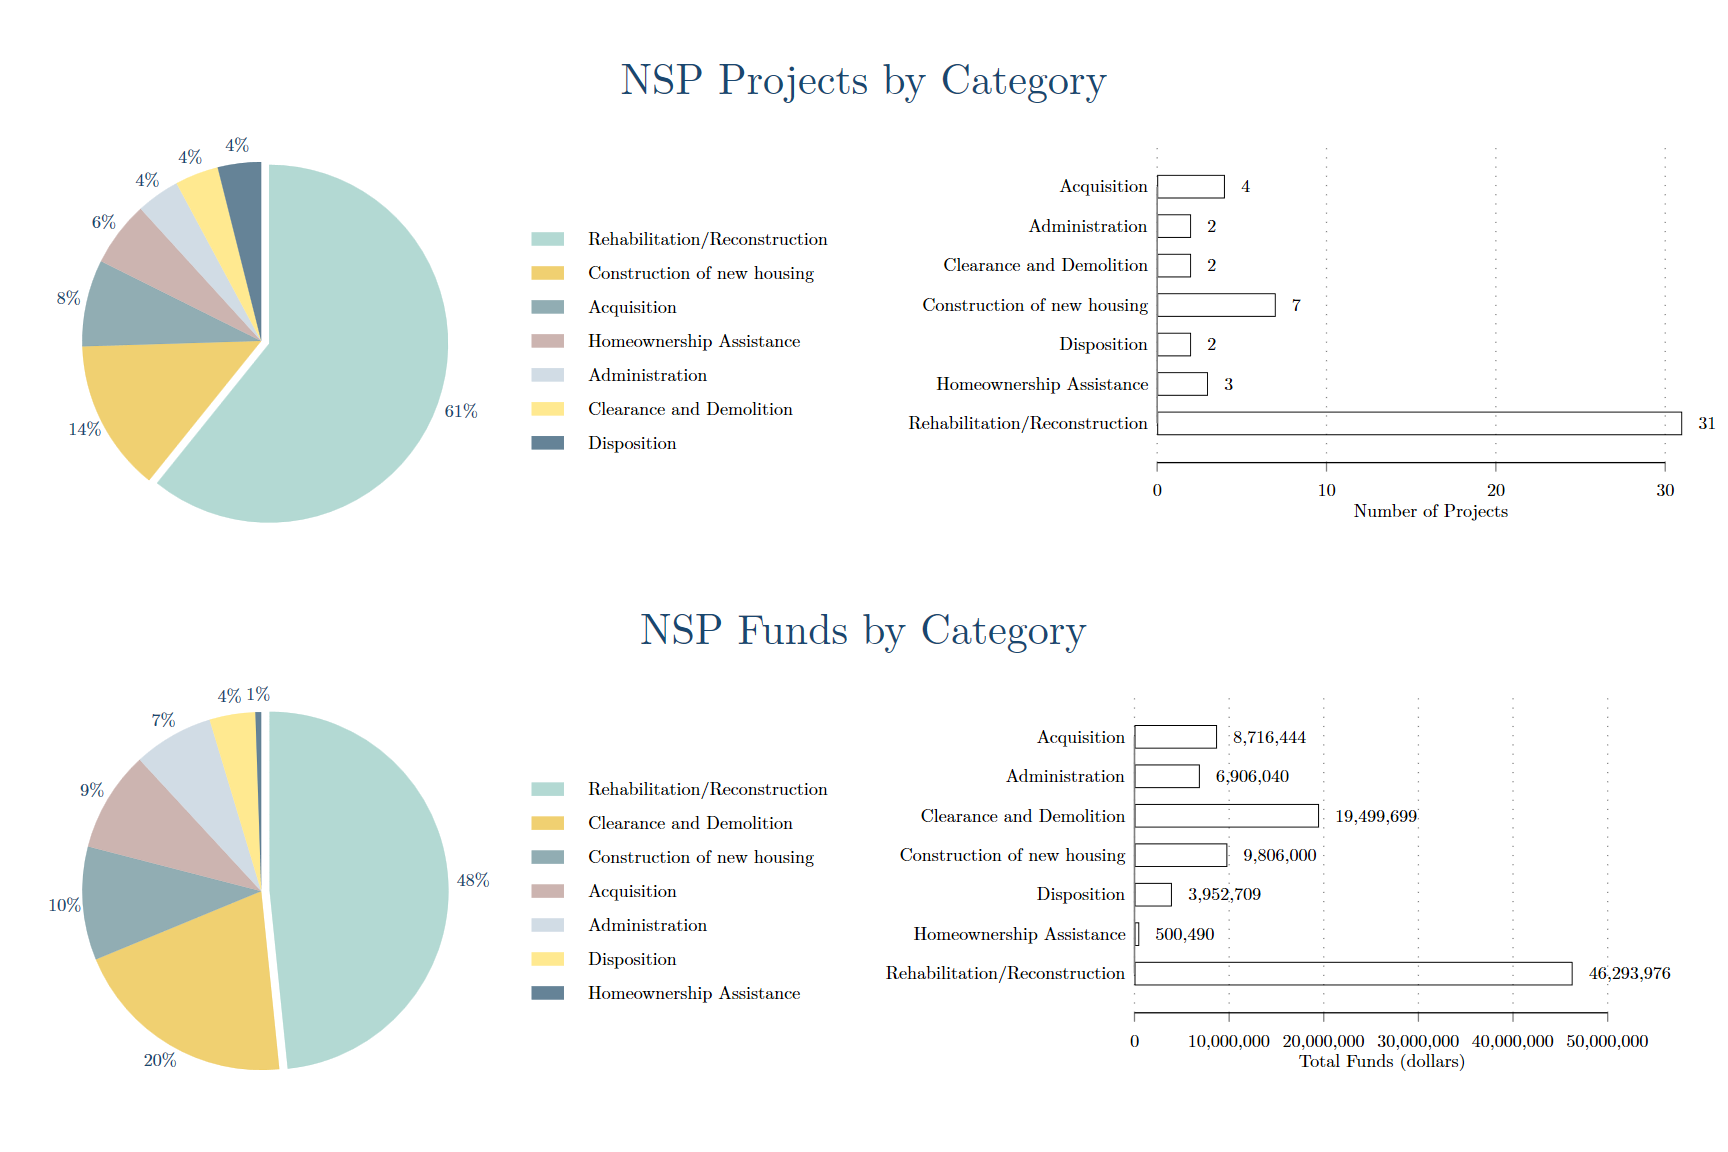
\includegraphics[width=0.8\textwidth]{nsp_projects_funds.png}
\caption{NSP Number of Projects and NSP Funds by Category of Activity in Detroit}
\label{fig:nsp_projects}
\begin{minipage}{\textwidth}
\footnotesize
\textit{Source:} Authors' calculations based on individual quarterly NSP performance reports provided by the City of Detroit.
\end{minipage}
\end{figure}


% =============================================================================
\section{Previous Work}
\label{sec:literature}
% =============================================================================

The central premise of the NSP implementation is that foreclosure properties contribute to negative externalities within neighborhoods which exacerbate urban blight \citep{spader2015}. The causal mechanisms include: (1)~the visual aspect of decay, creating a perception of an abandoned neighborhood and thereby decreasing neighboring property values; (2)~the consequential increase in the supply of properties due to foreclosures and subsequent vacancy, leading to an overall decline in market prices \citep{schuetz2015}; (3)~a negative perception of neighborhood safety as the number of foreclosed, abandoned, and deteriorated properties grows, which impacts the social infrastructure that can prevent criminal activity \citep{spader2016}; and (4)~a reduction in property tax revenues caused by lower assessed values, which subsequently impacts the provision of public goods and services, further lowering property values and perpetuating the vicious cycle \citep{johnson2008}. Empirical research confirms these negative impacts on property values \citep{lee2008,harding2009,campbell2011,anenberg2014,hartley2014,gerardi2015,zhang2014}, crime rates \citep{spelman1993,ellen2013,kondo2018,stacy2018,larson2019}, and health outcomes \citep{leon2017,wangimmergluck2018,pearson2019}. \citet{frame2010} provides a comprehensive review of the literature on foreclosure spillovers, documenting the range of estimated price effects and the methodological challenges involved.

NSP aims to counteract these effects by demolishing, clearing, constructing new housing, and rehabilitating blighted properties. However, bridging the gap between removing negative externalities and achieving positive neighborhood outcomes, such as enhanced property values or decreased crime, presents a significant challenge. The effectiveness of the policy relies on a multitude of factors identified in previous studies, and it is crucial to recognize that the mere eradication of foreclosure-related negative externalities does not automatically guarantee a corresponding positive impact of equal magnitude in the surrounding properties \citep{alvayay2023}. As \citet{whitaker2013} demonstrate in the context of Cuyahoga County, different types of property distress---vacancy, tax delinquency, and foreclosure---generate distinct spillover patterns, suggesting that a single programmatic response may not address all channels of neighborhood decline.

The theoretical framework for understanding why place-based interventions may have limited effects in severely declining markets draws on the insights of \citet{glaeser2005}, who argue that the durability of housing creates an asymmetry between growing and declining cities. In declining markets, excess supply persists because housing is physically durable, creating a ``floor'' effect that limits the upside potential of demand-side interventions. This is particularly relevant for Detroit, where long-term population decline had created massive housing oversupply well before the foreclosure crisis \citep{alm2014}. The NSP, by focusing on demolition and rehabilitation, addressed both supply (through removal of excess units) and demand (through improved neighborhood quality), but the scale of the crisis may have overwhelmed these efforts.

Mixed evidence on the effectiveness of NSP is highlighted in three methodologically similar studies summarized in Table~\ref{tab:prior_studies}. \citet{schuetz2016} evaluated NSP2 at the census tract level across 28 grantees, using regression analysis to compare treated and control tracts, finding no impact in Wayne County and mixed results elsewhere; Cuyahoga County showed positive sales growth, while Miami had negative outcomes. \citet{spader2016} and \citet{bak2017} analyzed property-level impacts, employing a buffer zone approach for creating comparable treatment and control areas. \citet{spader2016} found that NSP demolitions in Cleveland reduced property crimes, with no significant findings in Chicago or Denver, whereas \citet{bak2017} observed a 14.3\% increase in sale prices near NSP projects in Chicago, suggesting a positive property value effect. HUD's own evaluation of NSP2 concluded that the program was too modestly funded relative to the scale of the housing markets it was intended to influence, and found no consistent evidence that NSP2 activities arrested the overall decline in home prices in targeted neighborhoods \citep{hudevaluation2015}.

Beyond the direct NSP evaluations, a growing body of work in the \textit{Journal of Housing Economics} and related outlets has deepened our understanding of the channels through which programs like the NSP might operate. \citet{whitaker2013} demonstrate that different forms of property distress---vacancy, tax delinquency, and foreclosure---generate distinct and additive spillover patterns in Cuyahoga County, with each additional distressed property within 500 feet reducing neighboring sale prices by 1--2\%. \citet{ihlanfeldt2016} examine the mechanisms underlying foreclosure externalities in Florida and find that the negative price effects stem primarily from physical deterioration of neglected properties rather than from supply-side effects, reinforcing the rationale for rehabilitation-oriented programs. \citet{cui2015} use regression discontinuity methods to estimate foreclosure spillovers and demonstrate that foreclosure externalities are substantial, with each additional nearby foreclosure reducing sale prices by roughly 1\%. Collectively, these studies establish that the negative spillovers the NSP was designed to combat are well-documented, but also that their magnitude varies substantially across neighborhood types and market conditions.

The question of whether place-based interventions can reverse neighborhood decline has been examined more broadly in the housing economics literature. \citet{aarland2017} use a quasi-experimental approach to evaluate area-based intervention programs in Norway, finding modest positive effects on house prices, but noting that the impacts depend critically on program scale relative to neighborhood need. In the context of the Low-Income Housing Tax Credit (LIHTC) program, \citet{diamond2019} show that LIHTC developments in low-income neighborhoods increase surrounding house prices by 6.5\% and attract racially and income diverse populations, suggesting that targeted housing investment can serve as an effective place-based revitalization tool. \citet{voith2022} extend this analysis to concentrated LIHTC development in Chicago, finding that both stand-alone and clustered developments generate positive price spillover effects that persist for at least 10 years.

The demolition channel is particularly relevant for Detroit, where approximately 30\% of NSP funds were allocated to clearance activities. \citet{alvayay2023} examine the impact of Detroit's large-scale Hardest Hit Fund demolition program, finding that the average effect of blight removal on nearby property prices is modest, with positive effects concentrated in areas with relatively low pre-existing blight levels. \citet{paredes2017} perform a cost-benefit analysis of Detroit demolitions and conclude that under existing market conditions, demolition costs exceed the present value of additional property tax revenues over a 50-year horizon. These findings suggest that in severely distressed markets, demolition alone may be insufficient to generate positive price responses, a conclusion consistent with the theoretical predictions of \citet{glaeser2005} regarding the durability of housing in declining cities.

\begin{table}[htbp]
\centering
\caption{Prior Studies on the Impact of NSP on Different Outcomes}
\label{tab:prior_studies}
\begin{threeparttable}
\small
\begin{tabularx}{\textwidth}{p{2.2cm}p{2.5cm}p{1.2cm}p{1.3cm}p{2.5cm}p{3cm}p{1cm}}
\toprule
Study & Outcome Variable & Unit & Period & Location & Results & NSP Round \\
\midrule
\citet{schuetz2016} & Growth rate in annual sales volume, vacant and distressed properties & Census Tract & 2009--2013 & IL, Cuyahoga OH, Los Angeles CA, Wayne MI (counties) & No significant results for Wayne County. & NSP2 \\
\addlinespace
\citet{spader2016} & Number of crimes & Property & 2008--2013 & Cleveland, Chicago, Denver & NSP demolitions in Cleveland: reduction of 0.08 property crimes/quarter. No significant effect in Chicago or Denver. & NSP1, NSP2 \\
\addlinespace
\citet{bak2017} & log(sale price) & Property & 2008--2014 & Chicago & Homes near NSP projects increased by 14.3\%. & NSP1--3 (rehab only) \\
\bottomrule
\end{tabularx}
\begin{tablenotes}[flushleft]
\footnotesize
\item \textit{Source:} Authors' own elaboration.
\end{tablenotes}
\end{threeparttable}
\end{table}

The mentioned studies differ in two main aspects, aside from the variation in key outcome variables. \citet{bak2017} consider all three rounds of NSP and use a longer time frame to estimate the effect. Time is a critical factor when evaluating such policies, as urban revitalization processes may take years to materialize \citep{galster2006,schuetz2015}. Additionally, they focus on the effects of NSP projects that resulted in property rehabilitation, which aims to restore a property to productive use \citep{collins2013} and is observed to have a positive impact on neighboring property values \citep{leonard2017,ganduri2021}. On the other hand, the impact of demolition on neighborhood dynamics can be more ambiguous. For example, research on the Detroit Demolition Program provides an interesting contrast. According to \citet{alvayay2023}, the program, which was applied nearly citywide, shows no overall positive impact on property prices. However, using the same information on demolitions, \citet{alvayay2020} found positive and short-term effects on tax compliance in surrounding properties.

Central to our study is the recognition of the staggered implementation of the NSP policy across different rounds. No study we have encountered thus far has explicitly considered this temporal variation within a modern DiD framework. As \citet{immergluck2013} identified, one of the key challenges with NSP1 implementation was the short 18-month timeline to obligate funds. This tight deadline proved overly ambitious for the execution of complex local redevelopment programs, forcing many recipients to rush their decisions \citep{immergluck2012}. Consequently, the selection process became more about meeting deadlines than effectively identifying and intervening in areas that could benefit most. Due to this rushed process, the first-round beneficiaries were substantially different from those of the third round. The staggered nature of NSP, therefore, presents a key consideration for evaluating its impacts, motivating our use of estimators specifically designed for this setting \citep{callaway2021,wooldridge2023,goodmanbacon2021}.


% =============================================================================
\section{Identification Strategy}
\label{sec:identification}
% =============================================================================

\subsection{Empirical Framework}

In order to identify the effect of NSP policy on different outcomes, we define $Y_{it}$ as the dependent variable for census block group $i$ in year $t$. We evaluate the policy on two key variables: (1)~the log of the average residential property sale price, $\ln(\text{price})_{it}$, and (2)~the foreclosure rate, $\text{forerate}_{it}$. Census block groups are categorized into three groups based on treatment timing: never treated (control, $N = 399$), NSP1 zones (first treated in 2009, $N = 599$), and NSP3 zones (first treated in 2011, $N = 68$).

Our primary estimator is the \citet{callaway2021} difference-in-differences estimator for settings with multiple time periods and staggered treatment adoption. This estimator properly handles the well-documented biases that arise from using traditional TWFE models when treatment effects are heterogeneous across cohorts and over time \citep{dechaisemartin2020,goodmanbacon2021,roth2023}. With two treatment cohorts and a never-treated group, the staggered design is a natural fit: NSP3 block groups serve as not-yet-treated controls during 2006--2010, contributing additional identifying variation.

The Callaway and Sant'Anna estimator identifies group-time average treatment effects, $ATT(g,t)$, for each cohort $g$ (defined by the first period of treatment) and each time period $t$:
\begin{equation}
ATT(g,t) = \mathbb{E}[Y_t(g) - Y_t(0) \mid G_g = 1]
\label{eq:att_gt}
\end{equation}
where $Y_t(g)$ is the potential outcome under treatment adoption at time $g$, $Y_t(0)$ is the potential outcome under no treatment, and $G_g = 1$ indicates belonging to the cohort first treated at time $g$.

In our setting with two treatment cohorts ($g \in \{2009, 2011\}$), the overall average treatment effect on the treated aggregates across both groups and all post-treatment periods:
\begin{equation}
ATT = \sum_{g} \frac{N_g}{N_{\text{treated}}} \cdot \frac{1}{|\mathcal{T}_{g,\text{post}}|}\sum_{t \in \mathcal{T}_{g,\text{post}}} ATT(g, t)
\label{eq:att_overall}
\end{equation}
where $\mathcal{T}_{g,\text{post}}$ denotes the post-treatment periods for cohort $g$. This aggregation allows us to recover both the overall ATT and cohort-specific ATTs, providing insight into whether the program's effects varied with the timing of implementation.

\subsection{Addressing Selection Bias Through HUD Formula Variables}

A central challenge in evaluating the NSP is that targeted neighborhoods were systematically selected based on observable distress indicators. Detroit's local officials used criteria derived from HUD guidelines and local data to designate NSP target zones (see Table~\ref{tab:selection_criteria} in the Appendix). These criteria included: (1)~being in a low/moderate/middle-income (LMMH) area, (2)~having high foreclosure rates based on HUD data, (3)~having a high percentage of subprime mortgage-related loans, and (4)~alignment with citywide policies from the Master Plan \citep{pdd2009}.

HUD provided grantees with block group-level data including a composite risk score, predicted foreclosure rates, subprime loan rates, and residential vacancy rates. In our data, the HUD risk score is essentially constant across all Detroit block groups (mean $= 9.87$, with the 25th, 50th, 75th, and 90th percentiles all equal to 10), reflecting the fact that the entire city qualified as highly distressed. However, there is meaningful variation in the underlying formula components---the predicted foreclosure rate ($\text{predicted\_foreclo}$), subprime loan rate ($\text{loan\_rate}$), and residential vacancy rate ($\text{usps\_resid\_vac}$)---which exhibit strong relationships with treatment assignment.

We address the selection problem by including both HUD formula variables and baseline demographic characteristics as covariates in the Callaway and Sant'Anna estimator:
\begin{equation}
ATT(g,t) = \mathbb{E}\left[Y_t(g) - Y_t(0) \mid G_g = 1, X_i\right]
\label{eq:att_controls}
\end{equation}
where $X_i = (\text{predicted\_foreclo}_i, \text{loan\_rate}_i, \text{usps\_resid\_vac}_i, \text{pc\_black}_i, \text{mhi}_i)$ includes both the HUD formula variables and baseline demographic characteristics (percent Black and median household income in 2009). This specification implements the doubly robust estimator of \citet{callaway2021}, which combines outcome regression with inverse probability weighting to achieve consistent estimation if either the outcome model or the propensity score model is correctly specified. As a robustness check, we also estimate a specification with only the HUD formula variables in the propensity score (see Section~\ref{subsec:main_results}).

The importance of these controls is demonstrated by comparing results with and without them. Without any controls, we find large and statistically significant effects: a $-7.2\%$ effect on log sale prices ($p = 0.125$) and a $+22.4$ percentage point effect on foreclosure rates ($p < 0.001$). These large estimates reflect the fact that NSP1 areas had significantly higher predicted foreclosure rates (mean $= 21.3$ vs.~$15.9$ for controls, $p < 0.001$), higher subprime loan rates ($74.9\%$ vs.~$66.8\%$, $p < 0.001$), higher residential vacancy rates ($19.5\%$ vs.~$16.5\%$, $p < 0.001$), and a higher share of Black residents ($82.4\%$ vs.~$79.3\%$, $p = 0.001$). Once these variables are included, the estimated effects shrink dramatically, confirming that the unconditioned estimates were driven by selection on observables rather than causal program effects.

\subsection{Identification Assumptions}

The key identifying assumptions are:

\textbf{Conditional Parallel Trends.} In the absence of treatment, outcomes in the treated and control census block groups would have followed parallel trends over time, conditional on the covariates. We assess this assumption using pre-trend tests and event study plots. For our preferred specification (log sale prices with HUD and demographic controls), the pre-trend test yields $\chi^2(8) = 10.22$ ($p = 0.190$), failing to reject parallel pre-trends. For the foreclosure rate, the pre-trend test yields $\chi^2(8) = 7.65$ ($p = 0.265$), also providing no evidence against parallel trends. Figure~\ref{fig:trends_lprice} provides visual support: the log sale price trajectories for the three groups are approximately parallel in the pre-treatment period, although NSP3 areas operate at a higher level. In levels (Appendix Figure~\ref{fig:trends_levels}), the trends are less parallel, motivating the log transformation.

\textbf{No Anticipation.} Census block groups did not alter their behavior in anticipation of NSP treatment. Given the rapid deployment timeline of NSP1---with HUD's 18-month obligation deadline creating a rushed decision process \citep{immergluck2013}---substantial anticipation effects are unlikely. We use the ``not-yet-treated'' control group specification, which allows the control group to include units that will be treated in later periods (NSP3 areas serve as controls during 2006--2010), as an additional check.

\subsection{Robustness Estimators}

We complement the Callaway and Sant'Anna estimates with two additional approaches:

\textbf{Augmented Inverse Probability Weighting (AIPW).} We implement the \citet{wooldridge2023} heterogeneous treatment effects estimator via \texttt{xthdidregress} in Stata. This doubly robust estimator incorporates a richer set of covariates including, in addition to the HUD formula variables, baseline demographic characteristics (percent Black, median household income, distance to CBD).

\textbf{Traditional Two-Way Fixed Effects (TWFE).} We present standard panel fixed effects estimates as a benchmark, noting that in our setting with a single treatment cohort, the TWFE bias documented by \citet{goodmanbacon2021} is less severe than in settings with multiple treatment cohorts. We estimate:
\begin{equation}
Y_{it} = \alpha_i + \gamma_t + \beta \cdot \text{NSP1}_{it} + X_i' \delta_t + \varepsilon_{it}
\label{eq:twfe}
\end{equation}
where $\alpha_i$ and $\gamma_t$ are block group and year fixed effects, $\text{NSP1}_{it}$ is a binary indicator equal to 1 for NSP1 block groups in post-2009 years, and $X_i' \delta_t$ allows the HUD formula variables to have time-varying effects. Standard errors are clustered at the block group level.

\subsection{Log Transformation of Sale Prices}

Following standard practice in the housing economics literature, we use the natural logarithm of average sale prices as our primary outcome variable. The log transformation addresses several empirical concerns. First, the distribution of sale prices in Detroit is highly right-skewed, with a long tail of high-value transactions. Second, the log specification improves the plausibility of parallel trends---our diagnostic analysis shows that raw price trends are non-parallel in levels but substantially more parallel in logs. Third, the log specification provides estimates that are interpretable as approximate percentage changes.


% =============================================================================
\section{Data}
\label{sec:data}
% =============================================================================

\subsection{Data Sources}

This analysis focuses on 1,066 census block groups in Detroit, spanning from 2006 to 2019, creating a balanced panel of 14,924 observations. The staggered implementation of the NSP provides two treatment cohorts: 599 block groups first treated under NSP1 in 2009, and 68 block groups first treated under NSP3 in 2013, with 399 block groups that never received treatment serving as controls. This staggered timing is central to our identification strategy, as the \citet{callaway2021} estimator exploits the variation in treatment adoption across cohorts. Table~\ref{tab:variables} in the Appendix describes all the variables used in the analysis, the time interval, the geographic level, and the source.

We use information on residential property sale prices, foreclosure counts, and foreclosure rates within each census block group, sourced from ZTRAX \citep{zillow2020} and Data Driven Detroit. Key independent variables include property characteristics and geographical features derived from GIS and City of Detroit data, alongside time-variant controls like property age, lot size, and other housing features. The HUD formula variables---predicted foreclosure rates, subprime loan rates, and residential vacancy rates---are sourced from the HUD NSP allocation data \citep{hud2008} and serve as our primary controls for selection. Additional analysis leverages demographic and housing data from the American Community Survey, adjusted for 2000 and 2010 census geographies \citep{logan2014}.

\subsection{Data Description}

Figures~\ref{fig:trends_sale} and~\ref{fig:trends_fore} present descriptive trends for the two key outcome variables across the three groups: never-treated block groups, the NSP1 cohort (treated in 2009), and the NSP3 cohort (treated in 2013). Figure~\ref{fig:trends_sale} shows average log sale prices over time. Prior to 2009, the three groups follow broadly similar trajectories, with all experiencing sharp declines during the foreclosure crisis. After treatment, NSP1 areas show somewhat lower prices, consistent with the selection mechanism that directed funds to the most distressed neighborhoods. The NSP3 cohort tracks above the other two groups throughout the sample period, reflecting the different neighborhood characteristics of the later round.

\begin{figure}[htbp]
\centering
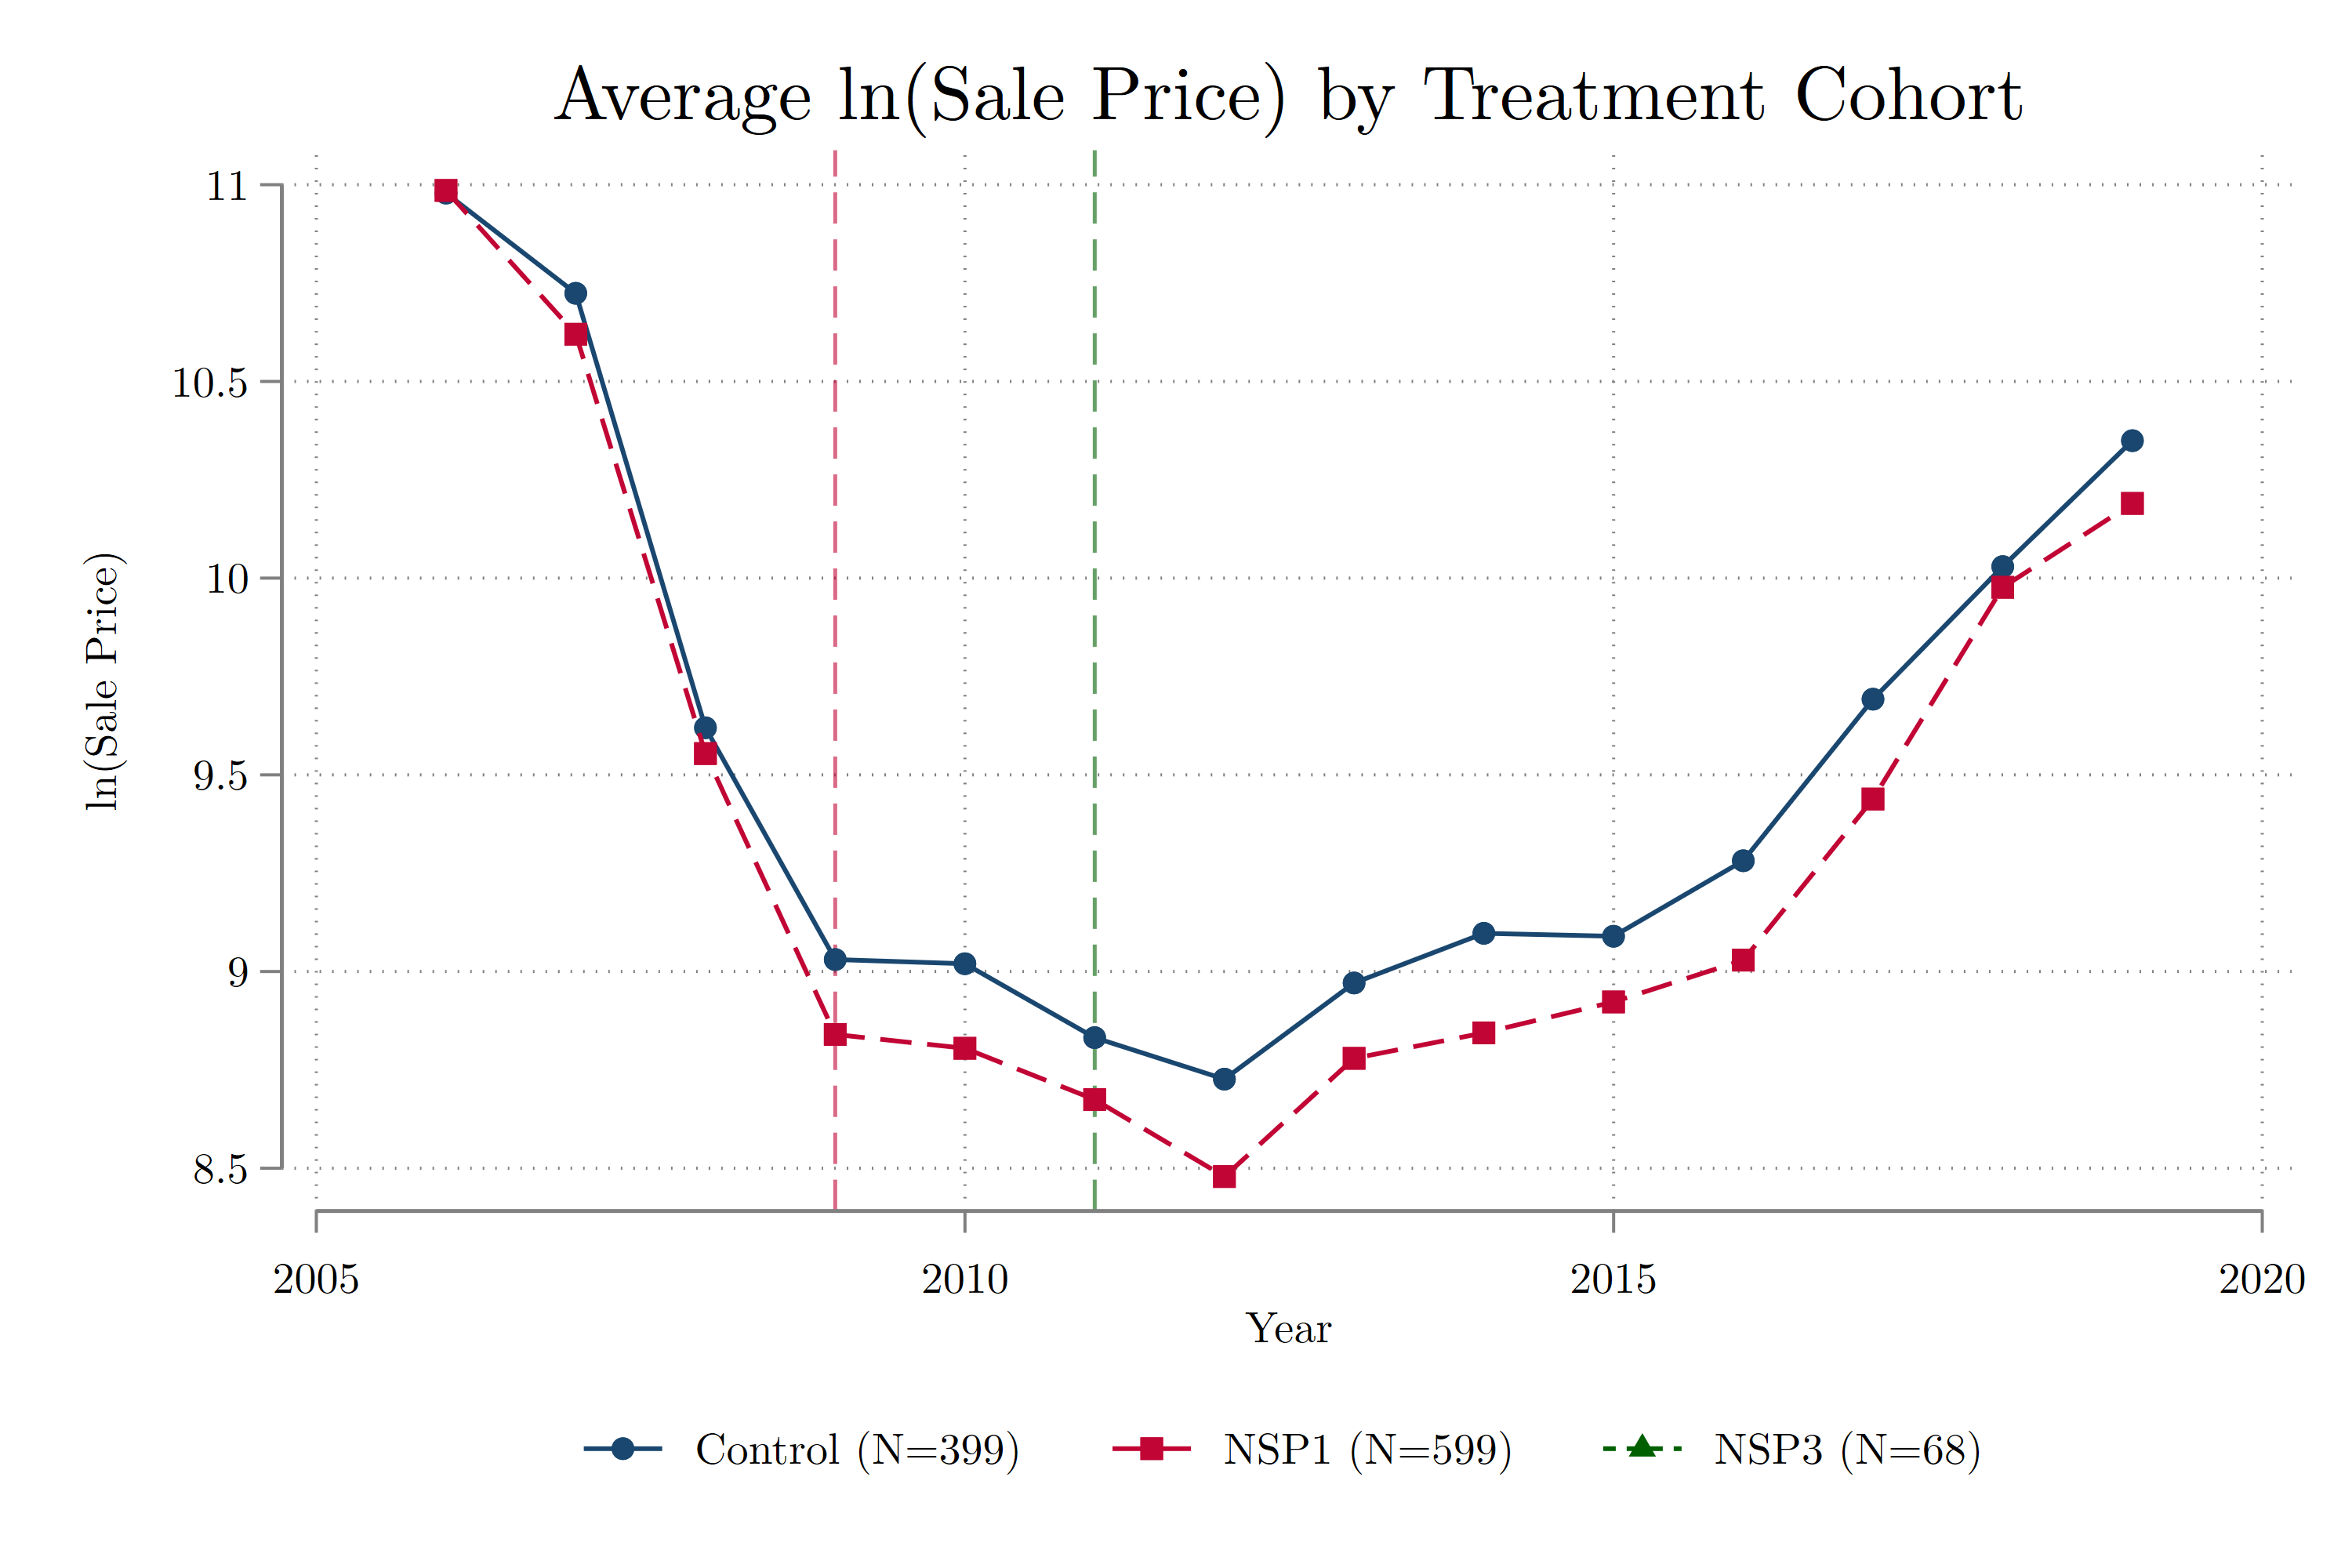
\includegraphics[width=0.85\textwidth]{pretrend_lprice_staggered.png}
\caption{Descriptive Trends: Average ln(Sale Price) by Treatment Cohort}
\label{fig:trends_sale}
\begin{minipage}{\textwidth}
\footnotesize
\textit{Source:} Authors' calculations. \textit{Note:} The figure presents average ln(sale price) trajectories for never-treated block groups ($N = 399$), NSP1 block groups treated in 2009 ($N = 599$), and NSP3 block groups treated in 2013 ($N = 68$). Vertical dashed lines mark the respective treatment years.
\end{minipage}
\end{figure}

Figure~\ref{fig:trends_fore} shows the analogous comparison for foreclosure rates. The three groups track closely throughout, with rates rising sharply during the crisis period (2007--2009) and then declining gradually. The close alignment of these unconditional trends is notable, though the formal pre-trend test within the Callaway and Sant'Anna framework---which conditions on the HUD formula variables---provides the appropriate statistical test of the identifying assumption ($p = 0.066$ for foreclosure rates; $p = 0.121$ for log sale prices).

\begin{figure}[htbp]
\centering
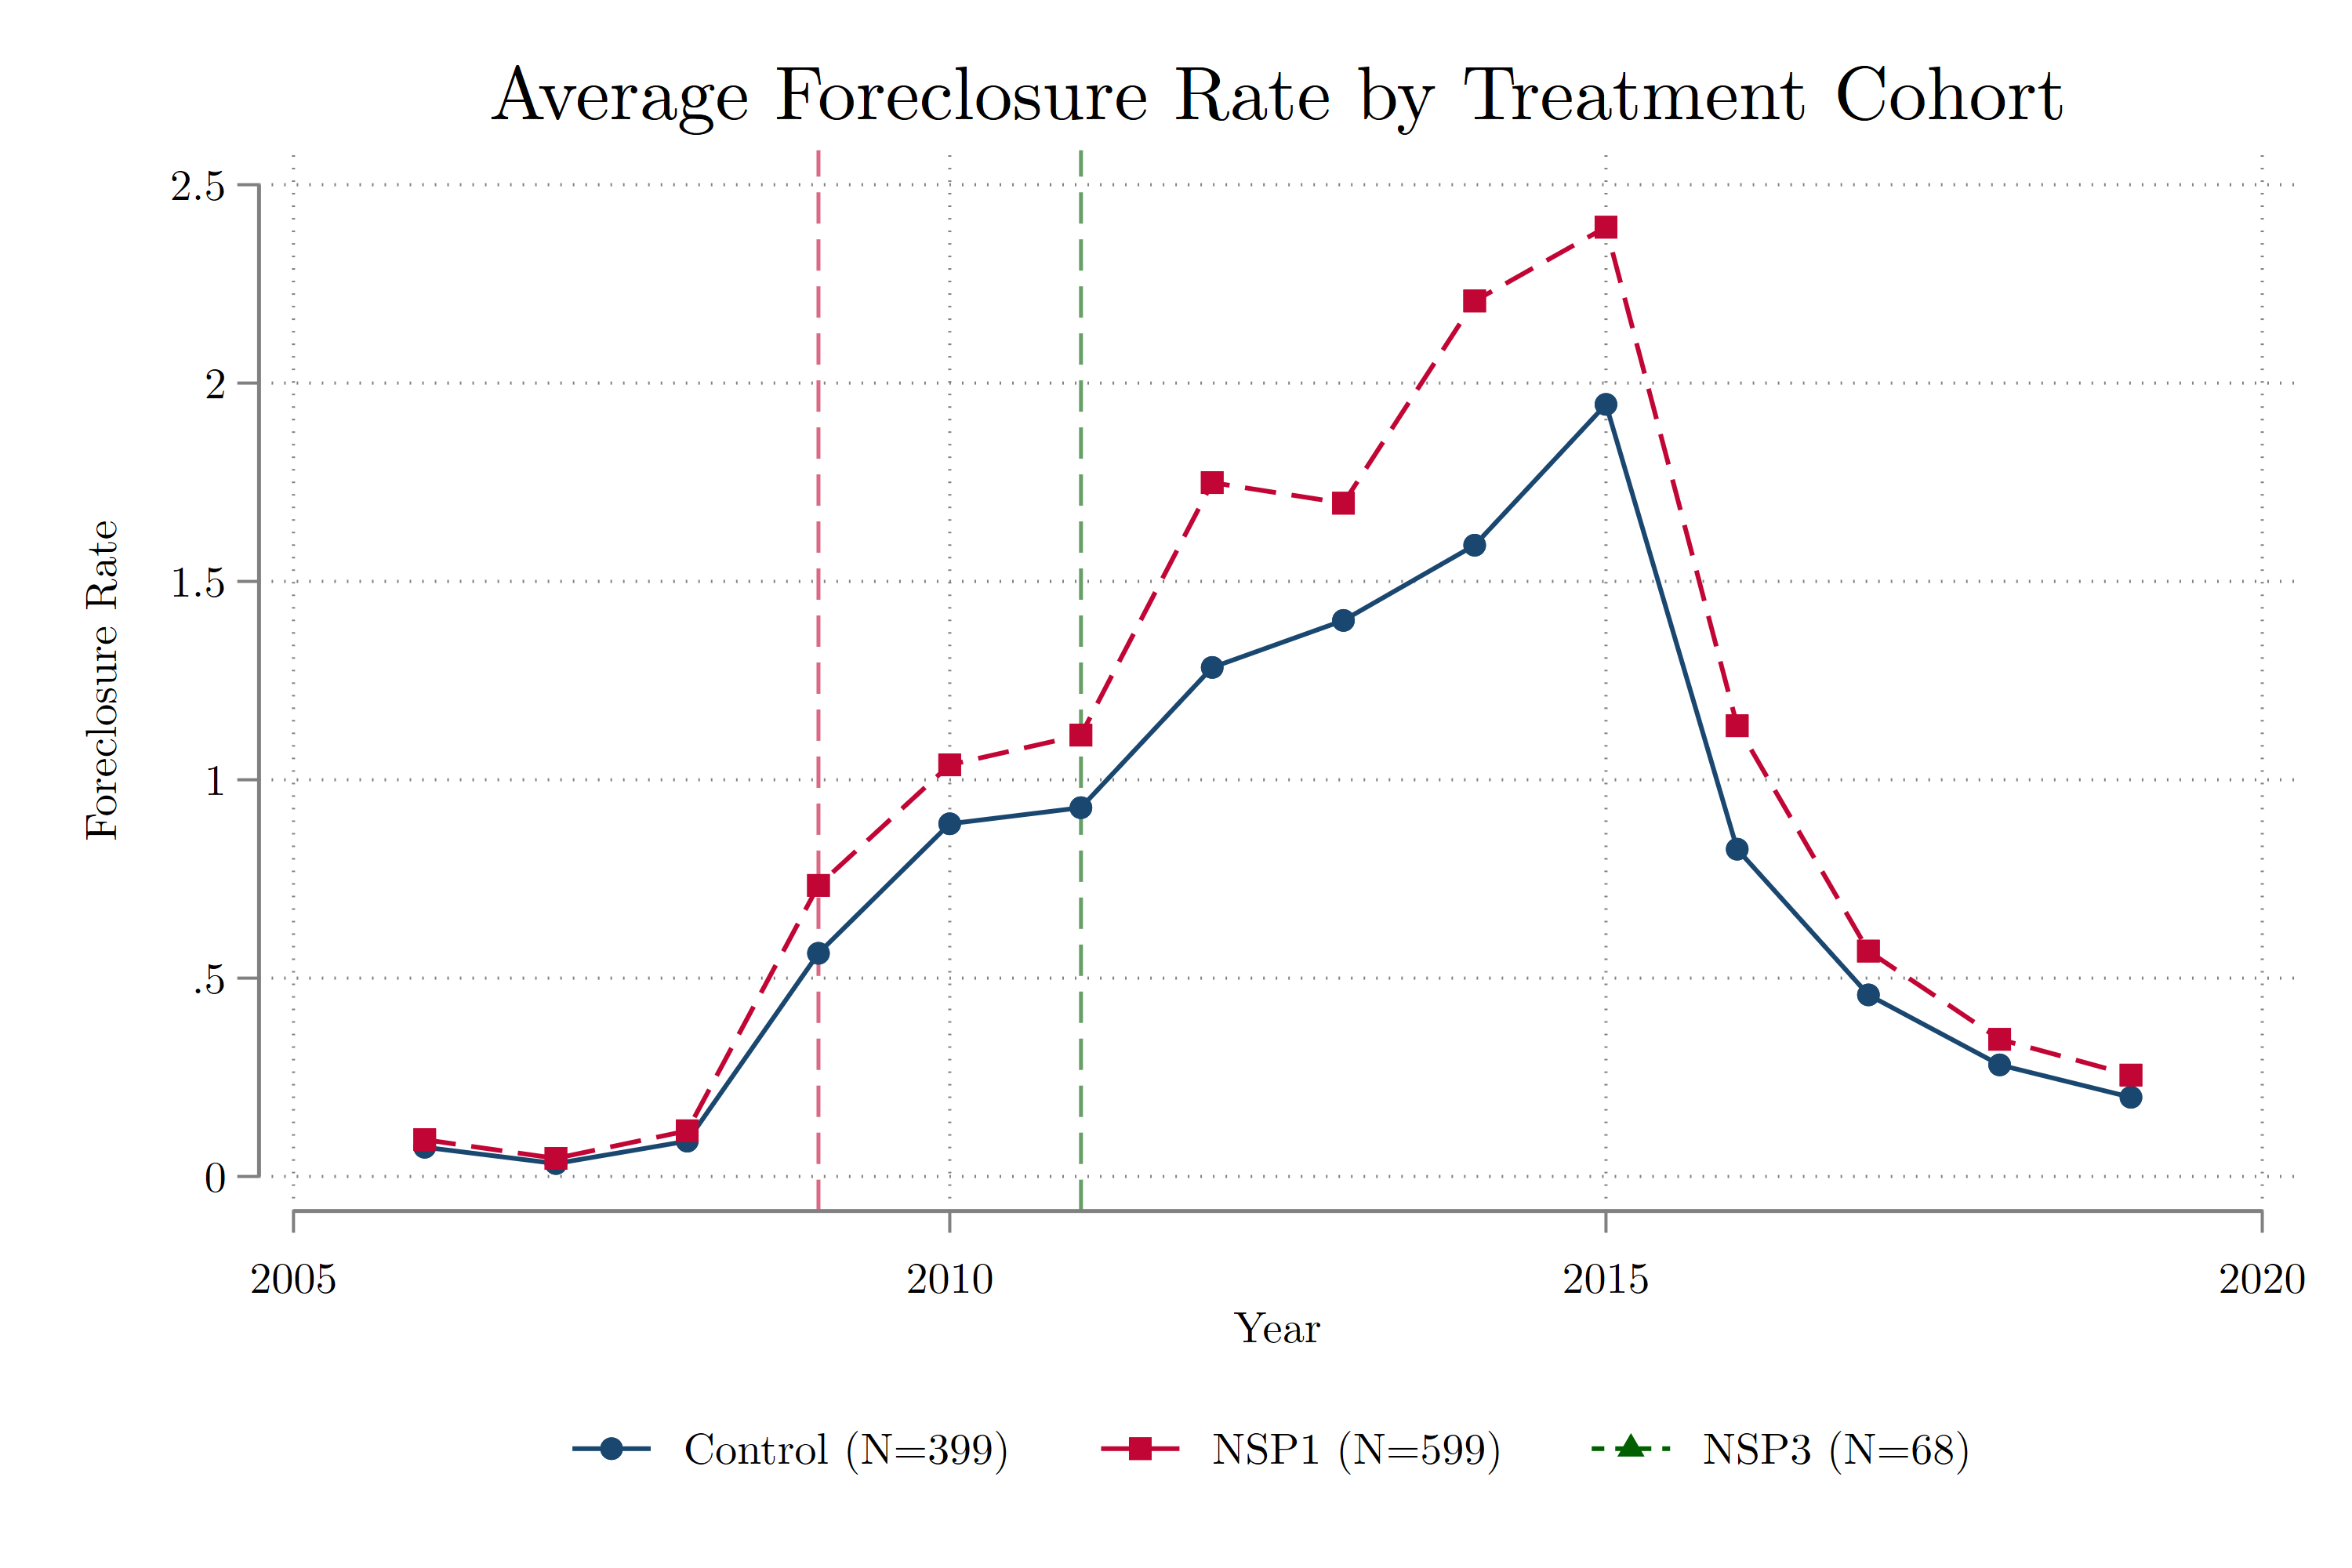
\includegraphics[width=0.85\textwidth]{pretrend_forerate_staggered.png}
\caption{Descriptive Trends: Average Foreclosure Rate by Treatment Cohort}
\label{fig:trends_fore}
\begin{minipage}{\textwidth}
\footnotesize
\textit{Source:} Authors' calculations. \textit{Note:} The figure presents average foreclosure rate trajectories for never-treated block groups ($N = 399$), NSP1 block groups treated in 2009 ($N = 599$), and NSP3 block groups treated in 2013 ($N = 68$). Vertical dashed lines mark the respective treatment years.
\end{minipage}
\end{figure}

Table~\ref{tab:summary} provides summary statistics at baseline (2008) for all three groups. NSP1 areas have lower average sale prices (\$19,798 vs.\ \$23,352 for controls), higher foreclosure rates (0.12 vs.\ 0.09), and are significantly different on the HUD formula variables. NSP3 areas present a different profile: they have higher median household incomes (\$39,235), lower vacancy rates (13.63\%), and lower predicted foreclosure rates (14.72) than controls, suggesting that the third round targeted areas with greater revitalization potential rather than acute distress. These systematic differences across groups underscore the need for controlling for the selection mechanism and motivate the cohort-specific analysis.

\begin{table}[htbp]
\centering
\caption{Summary Statistics at Baseline (2008): Control, NSP1, and NSP3}
\label{tab:summary}
\begin{threeparttable}
\small
\begin{tabular}{lrrrrrr}
\toprule
& \multicolumn{2}{c}{Control ($N = 399$)} & \multicolumn{2}{c}{NSP1 ($N = 599$)} & \multicolumn{2}{c}{NSP3 ($N = 68$)} \\
\cmidrule(lr){2-3} \cmidrule(lr){4-5} \cmidrule(lr){6-7}
Variable & Mean & Std.\ Dev. & Mean & $p$\textsuperscript{a} & Mean & $p$\textsuperscript{b} \\
\midrule
Sale Price (\$) & 23,352 & 25,768 & 19,798 & $0.017^{**}$ & 32,425 & $0.020^{**}$ \\
ln(Sale Price) & 9.62 & 1.00 & 9.55 & $0.263$ & 10.04 & $0.003^{***}$ \\
Foreclosure Rate & 0.09 & 0.13 & 0.12 & $0.001^{***}$ & 0.07 & $0.230$ \\
Number of Sales & 12.85 & 10.24 & 16.17 & $< 0.001^{***}$ & 14.62 & $0.168$ \\
\addlinespace
\multicolumn{7}{l}{\textit{HUD Formula Variables}} \\
Predicted Foreclosure & 15.89 & --- & 21.33 & $< 0.001^{***}$ & 14.72 & $0.001^{***}$ \\
Subprime Loan Rate (\%) & 66.80 & --- & 74.94 & $< 0.001^{***}$ & 59.98 & $0.001^{***}$ \\
Residential Vacancy (\%) & 16.49 & --- & 19.45 & $< 0.001^{***}$ & 13.63 & $0.002^{***}$ \\
\addlinespace
\multicolumn{7}{l}{\textit{Demographic Variables}} \\
\% Black (2009) & 79.25 & --- & 82.36 & $0.001^{***}$ & 76.21 & $0.386$ \\
Median HH Income (\$) & 30,162 & --- & 28,519 & $0.090^{*}$ & 39,235 & $< 0.001^{***}$ \\
Distance to CBD (miles) & 6.91 & --- & 6.74 & $0.519$ & 7.39 & $0.239$ \\
\bottomrule
\end{tabular}
\begin{tablenotes}[flushleft]
\footnotesize
\item \textit{Source:} Authors' calculations. \textit{Note:} \textsuperscript{a}$p$-value for NSP1 vs.\ Control. \textsuperscript{b}$p$-value for NSP3 vs.\ Control. Two-sample $t$-tests of equality of means. HUD formula variables are time-invariant. $^{***} p < 0.01$, $^{**} p < 0.05$, $^{*} p < 0.10$.
\end{tablenotes}
\end{threeparttable}
\end{table}


% =============================================================================
\section{Results}
\label{sec:results}
% =============================================================================

\subsection{Summary Statistics}

Table~\ref{tab:summary} provides summary statistics at baseline (2008) for the three groups: control, NSP1, and NSP3. NSP1 areas have lower average sale prices (\$19,798 vs.\ \$23,352 for controls, $p = 0.017$) and significantly higher foreclosure rates (0.12 vs.\ 0.09, $p = 0.001$). The HUD formula variables reveal the selection mechanism: NSP1 areas have higher predicted foreclosure rates (21.33 vs.\ 15.89, $p < 0.001$), higher subprime loan rates (74.94\% vs.\ 66.80\%, $p < 0.001$), and higher residential vacancy rates (19.45\% vs.\ 16.49\%, $p < 0.001$). NSP1 neighborhoods also have a significantly higher share of Black residents (82.36\% vs.\ 79.25\%, $p = 0.001$).

NSP3 areas present a different profile: they have higher median household incomes (\$39,235 vs.\ \$30,162, $p = 0.090$), lower vacancy rates, and lower predicted foreclosure rates than controls on most dimensions, suggesting that the third round targeted areas with greater revitalization potential rather than acute distress.

\subsection{Descriptive Trends}

Figures~\ref{fig:trends_lprice} and \ref{fig:trends_fore} present the average trajectories of log sale prices and foreclosure rates by treatment cohort. For log sale prices (Figure~\ref{fig:trends_lprice}), the three groups follow approximately parallel trends during 2006--2008, supporting the conditional parallel trends assumption. All groups experience a sharp decline during 2008--2010, with NSP1 areas declining more steeply. By 2019, the control group has recovered more strongly than NSP1, while NSP3 areas---which were less distressed at baseline---maintain their level advantage throughout.

For the foreclosure rate (Figure~\ref{fig:trends_fore}), the pre-treatment trends are closely aligned across all three groups, providing strong visual support for the parallel trends assumption. The post-treatment trajectories diverge modestly, with NSP1 areas showing somewhat higher foreclosure rates during the 2012--2015 period.

\begin{figure}[htbp]
\centering
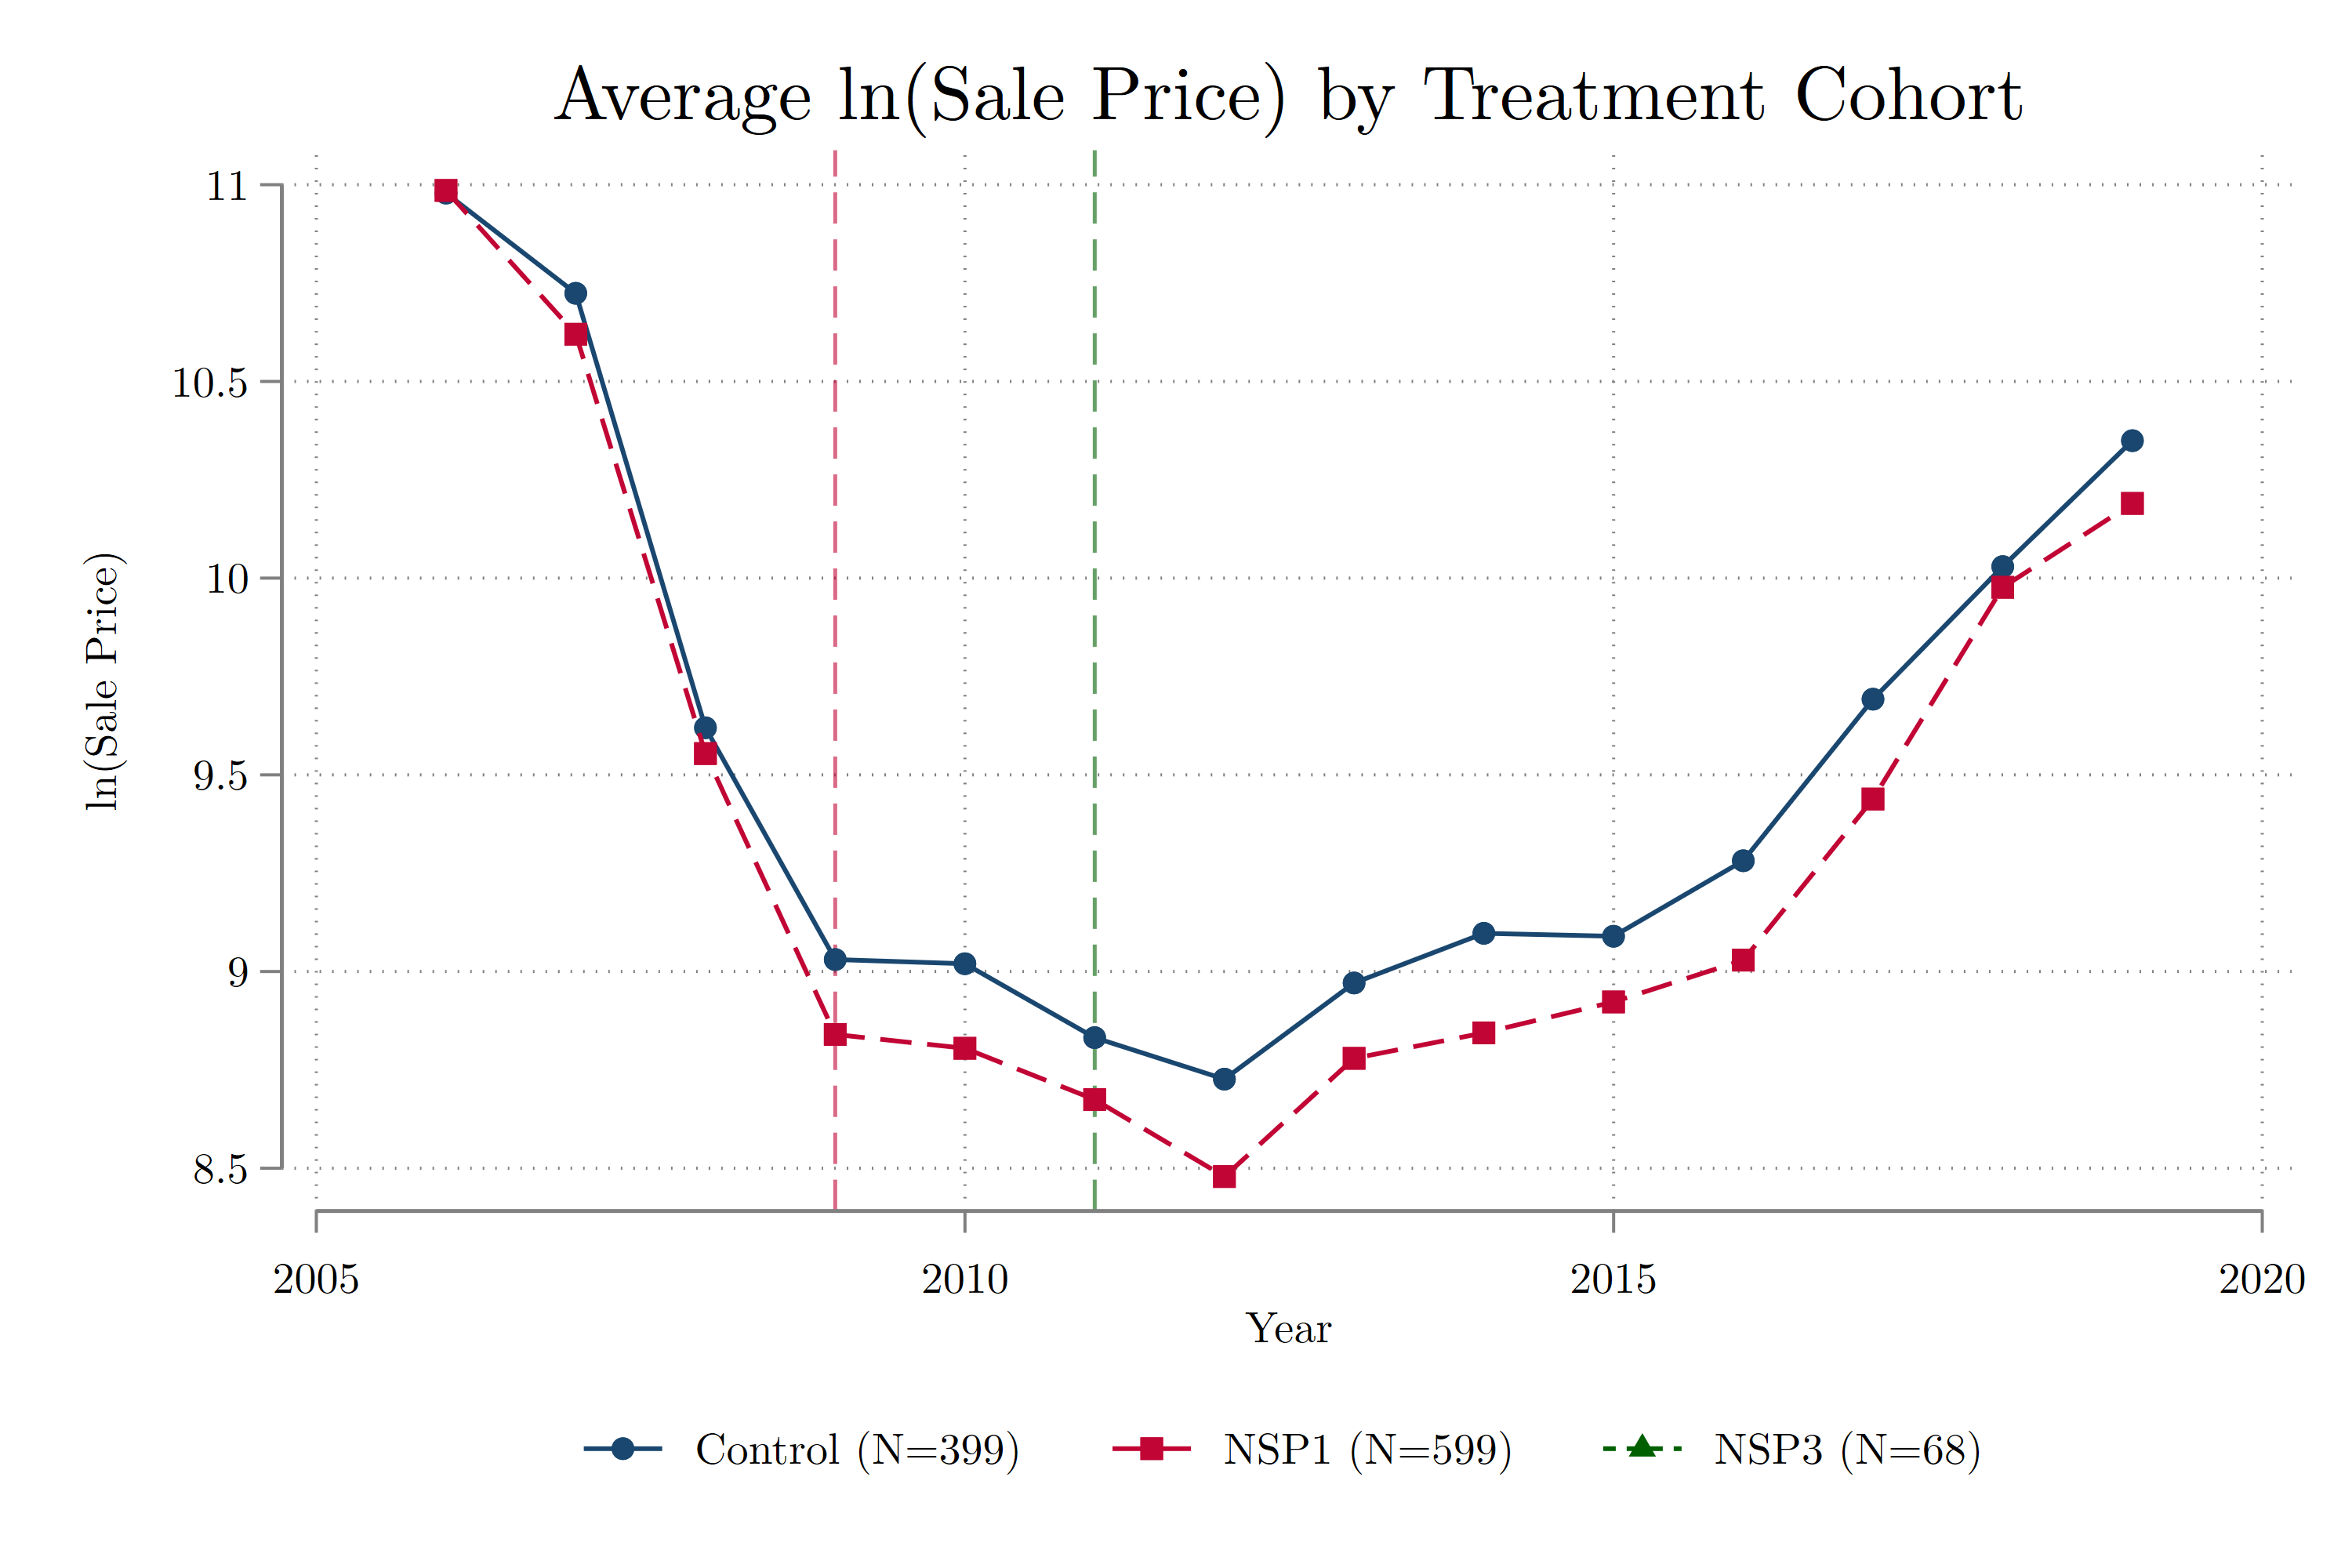
\includegraphics[width=0.85\textwidth]{pretrend_lprice_staggered.png}
\caption{Descriptive Trends: Average ln(Sale Price) by Treatment Cohort}
\label{fig:trends_lprice}
\begin{minipage}{\textwidth}
\footnotesize
\textit{Source:} Authors' calculations. \textit{Note:} The figure presents average ln(sale price) trajectories for never-treated block groups ($N = 399$), NSP1 block groups treated in 2009 ($N = 599$), and NSP3 block groups treated in 2011 ($N = 68$). Vertical dashed lines mark the respective treatment years.
\end{minipage}
\end{figure}

\begin{figure}[htbp]
\centering
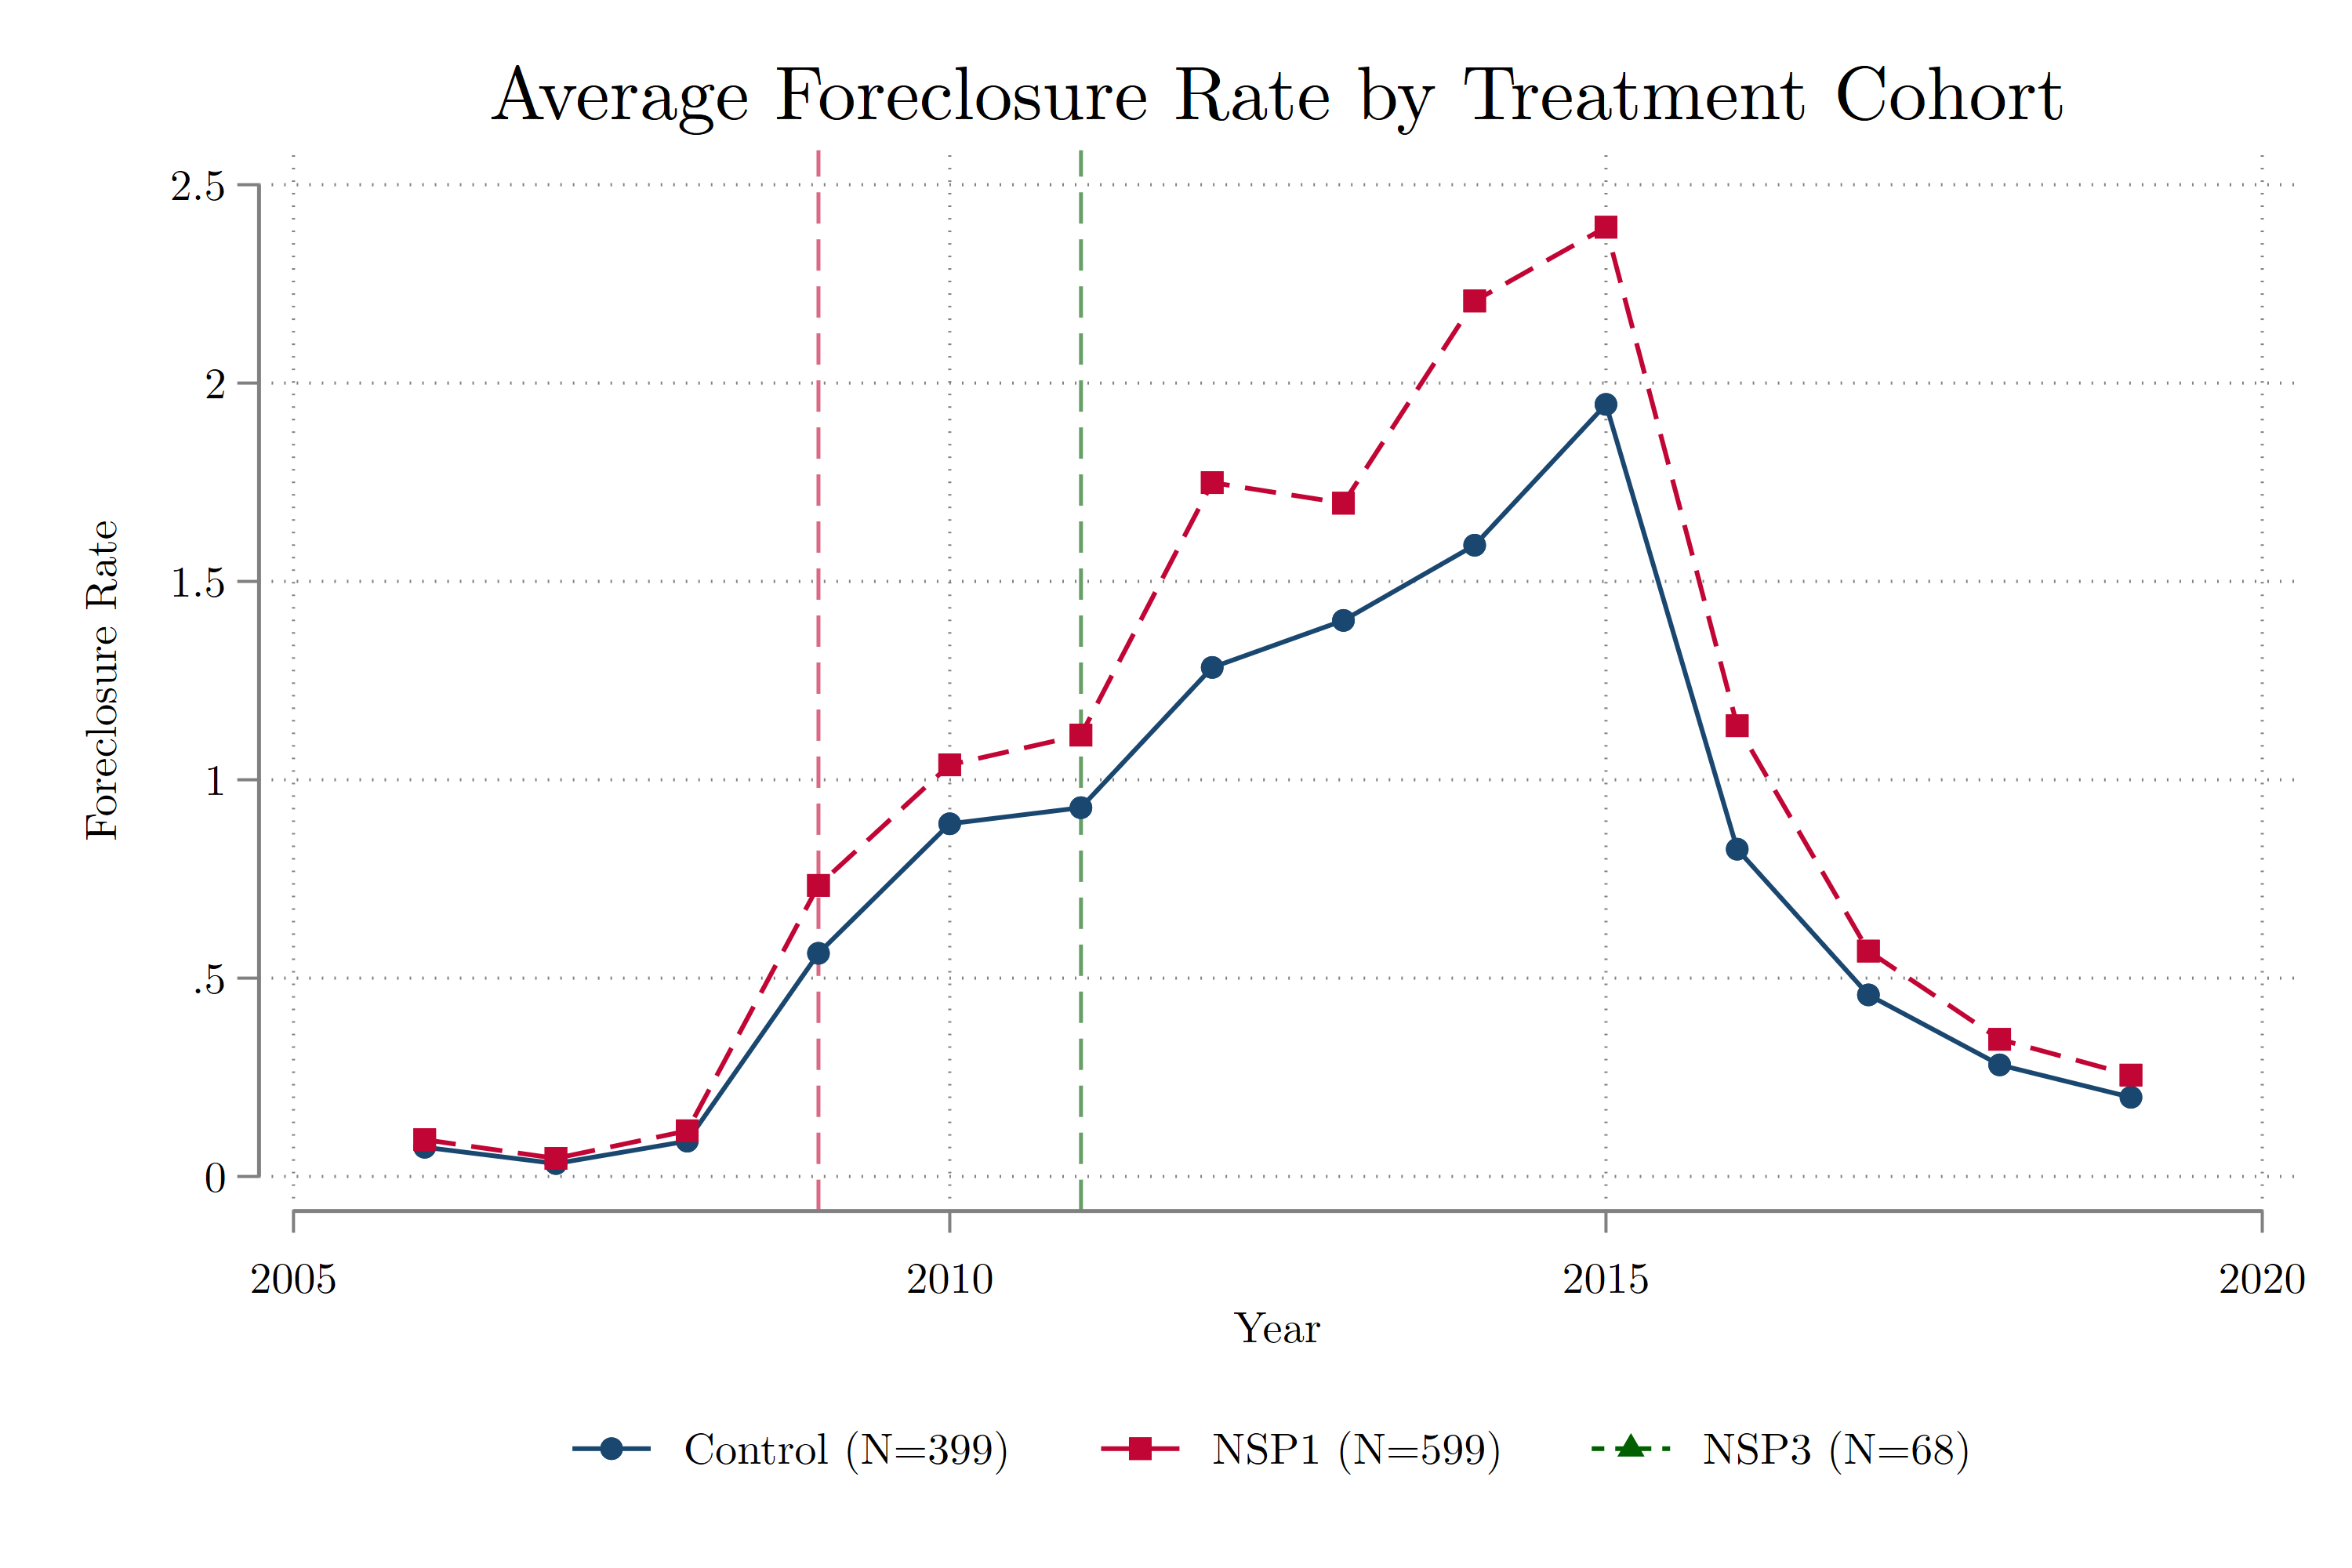
\includegraphics[width=0.85\textwidth]{pretrend_forerate_staggered.png}
\caption{Descriptive Trends: Average Foreclosure Rate by Treatment Cohort}
\label{fig:trends_fore}
\begin{minipage}{\textwidth}
\footnotesize
\textit{Source:} Authors' calculations. \textit{Note:} The figure presents average foreclosure rate trajectories for the three groups. Vertical dashed lines mark the respective treatment years.
\end{minipage}
\end{figure}

\subsection{Main Results: Propensity Score Sensitivity}
\label{subsec:main_results}

Table~\ref{tab:main_results} presents our main results from the \citet{callaway2021} estimator, which exploits the staggered timing of NSP1 (2009) and NSP3 (2011) to identify treatment effects using not-yet-treated and never-treated block groups as the comparison group.

Our preferred specification includes both HUD formula variables and demographic characteristics (percent Black, median household income) in the propensity score. The overall ATT for log sale prices is $-0.017$ ($\text{SE} = 0.053$, $p = 0.740$), indicating no statistically significant effect of the NSP on housing prices. For the foreclosure rate, the overall ATT is $+0.094$ ($\text{SE} = 0.049$, $p = 0.058$), suggesting a marginally significant increase in foreclosure rates in treated areas. The formal pre-trend tests fail to reject the null of parallel pre-treatment trends for both outcomes ($p = 0.190$ for prices, $p = 0.265$ for foreclosures), supporting the identification strategy.

As a robustness check, we estimate a specification with only HUD formula variables in the propensity score (without demographics). The results are nearly identical: $-0.013$ ($p = 0.803$) for prices and $+0.085$ ($p = 0.092$) for foreclosures, demonstrating that the results are not sensitive to the propensity score specification. Without any controls, the estimated effects are large and significant: $-0.072$ ($p = 0.125$) for prices and $+0.224$ ($p < 0.001$) for foreclosures---confirming that selection bias drives the unconditioned estimates.

\begin{table}[htbp]
\centering
\caption{Callaway and Sant'Anna Staggered DiD Estimates: Propensity Score Sensitivity}
\label{tab:main_results}
\begin{threeparttable}
\begin{tabular}{lcccc}
\toprule
& \multicolumn{2}{c}{ln(Sale Price)} & \multicolumn{2}{c}{Foreclosure Rate} \\
\cmidrule(lr){2-3} \cmidrule(lr){4-5}
& ATT & $p$-value & ATT & $p$-value \\
\midrule
\textbf{Main (HUD + Demographics)} & $-0.017$ & $0.740$ & $+0.094^{*}$ & $0.058$ \\
& $(0.053)$ & & $(0.049)$ & \\
\addlinespace
Robustness (HUD Only) & $-0.013$ & $0.803$ & $+0.085^{*}$ & $0.092$ \\
& $(0.053)$ & & $(0.052)$ & \\
\addlinespace
No Controls & $-0.072$ & $0.125$ & $+0.224^{***}$ & $<0.001$ \\
& $(0.047)$ & & $(0.042)$ & \\
\addlinespace
\midrule
Pre-trend $\chi^2$ (Main) & $10.22$ & $(p = 0.190)$ & $7.65$ & $(p = 0.265)$ \\
Pre-trend $\chi^2$ (HUD Only) & $12.74$ & $(p = 0.121)$ & $14.65^{*}$ & $(p = 0.066)$ \\
\addlinespace
Control group & \multicolumn{4}{c}{Not-yet treated + never treated} \\
Block groups & \multicolumn{4}{c}{$1{,}066$ (399 control, 599 NSP1, 68 NSP3)} \\
\bottomrule
\end{tabular}
\begin{tablenotes}[flushleft]
\footnotesize
\item \textit{Source:} Authors' calculations. \textit{Note:} Estimated using the \citet{callaway2021} estimator with doubly robust (IPW) inference and staggered treatment timing ($g = 2009$ for NSP1, $g = 2011$ for NSP3). Main specification includes predicted foreclosure rate, subprime loan rate, residential vacancy rate, percent Black, and median household income. Standard errors in parentheses. $^{***} p < 0.01$, $^{**} p < 0.05$, $^{*} p < 0.10$.
\end{tablenotes}
\end{threeparttable}
\end{table}

Figures~\ref{fig:sensitivity_sale} and \ref{fig:sensitivity_fore} present the event study comparison between the main specification (HUD + demographics) and the HUD-only robustness check. Both specifications produce nearly identical event-time paths for both outcomes, with overlapping confidence intervals at every horizon. For log sale prices, the pre-treatment coefficients are centered around zero, and post-treatment coefficients oscillate without a clear trend. For the foreclosure rate, the pre-treatment coefficients are well-behaved, while the post-treatment coefficients show a distinctive inverted-U pattern, peaking at 3--5 years after treatment.

\begin{figure}[htbp]
\centering
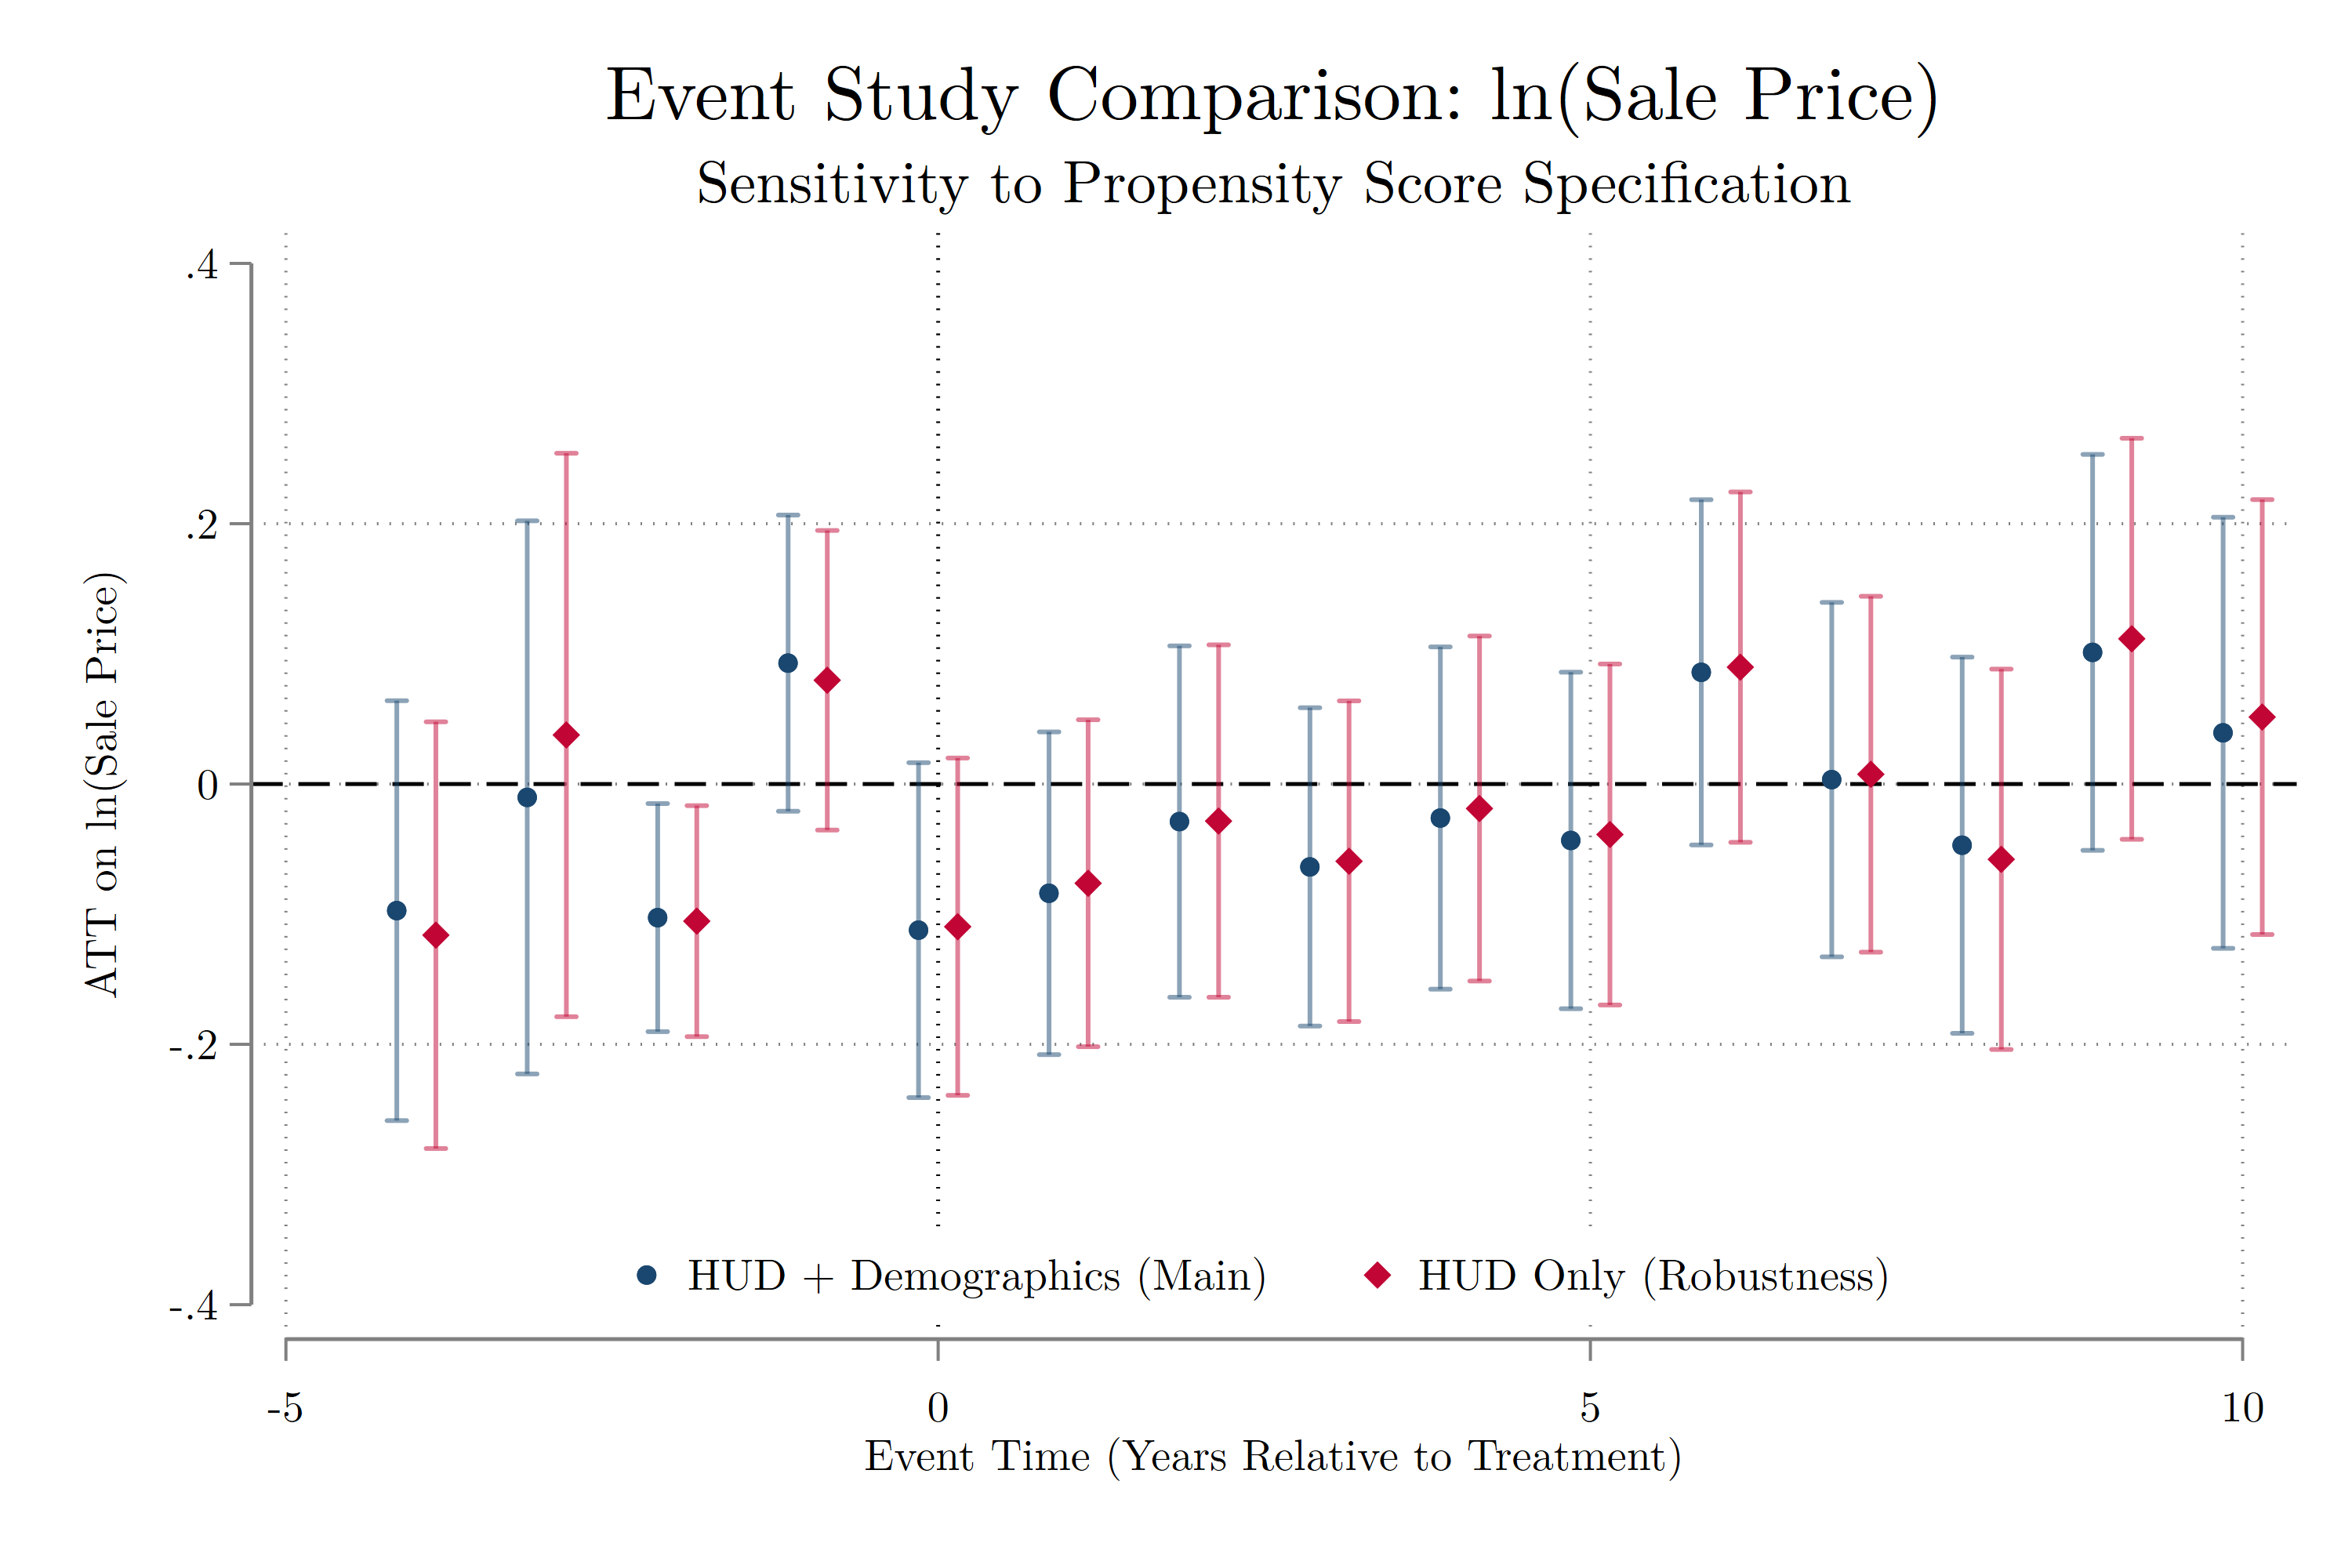
\includegraphics[width=0.85\textwidth]{cs_compare_specs_sale.png}
\caption{Event Study Comparison: ln(Sale Price) --- Sensitivity to Propensity Score Specification}
\label{fig:sensitivity_sale}
\begin{minipage}{\textwidth}
\footnotesize
\textit{Source:} Authors' calculations. \textit{Note:} Event study coefficients from the \citet{callaway2021} estimator with two propensity score specifications: HUD + Demographics (circles, navy) and HUD Only (diamonds, red). 95\% confidence intervals shown.
\end{minipage}
\end{figure}

\begin{figure}[htbp]
\centering
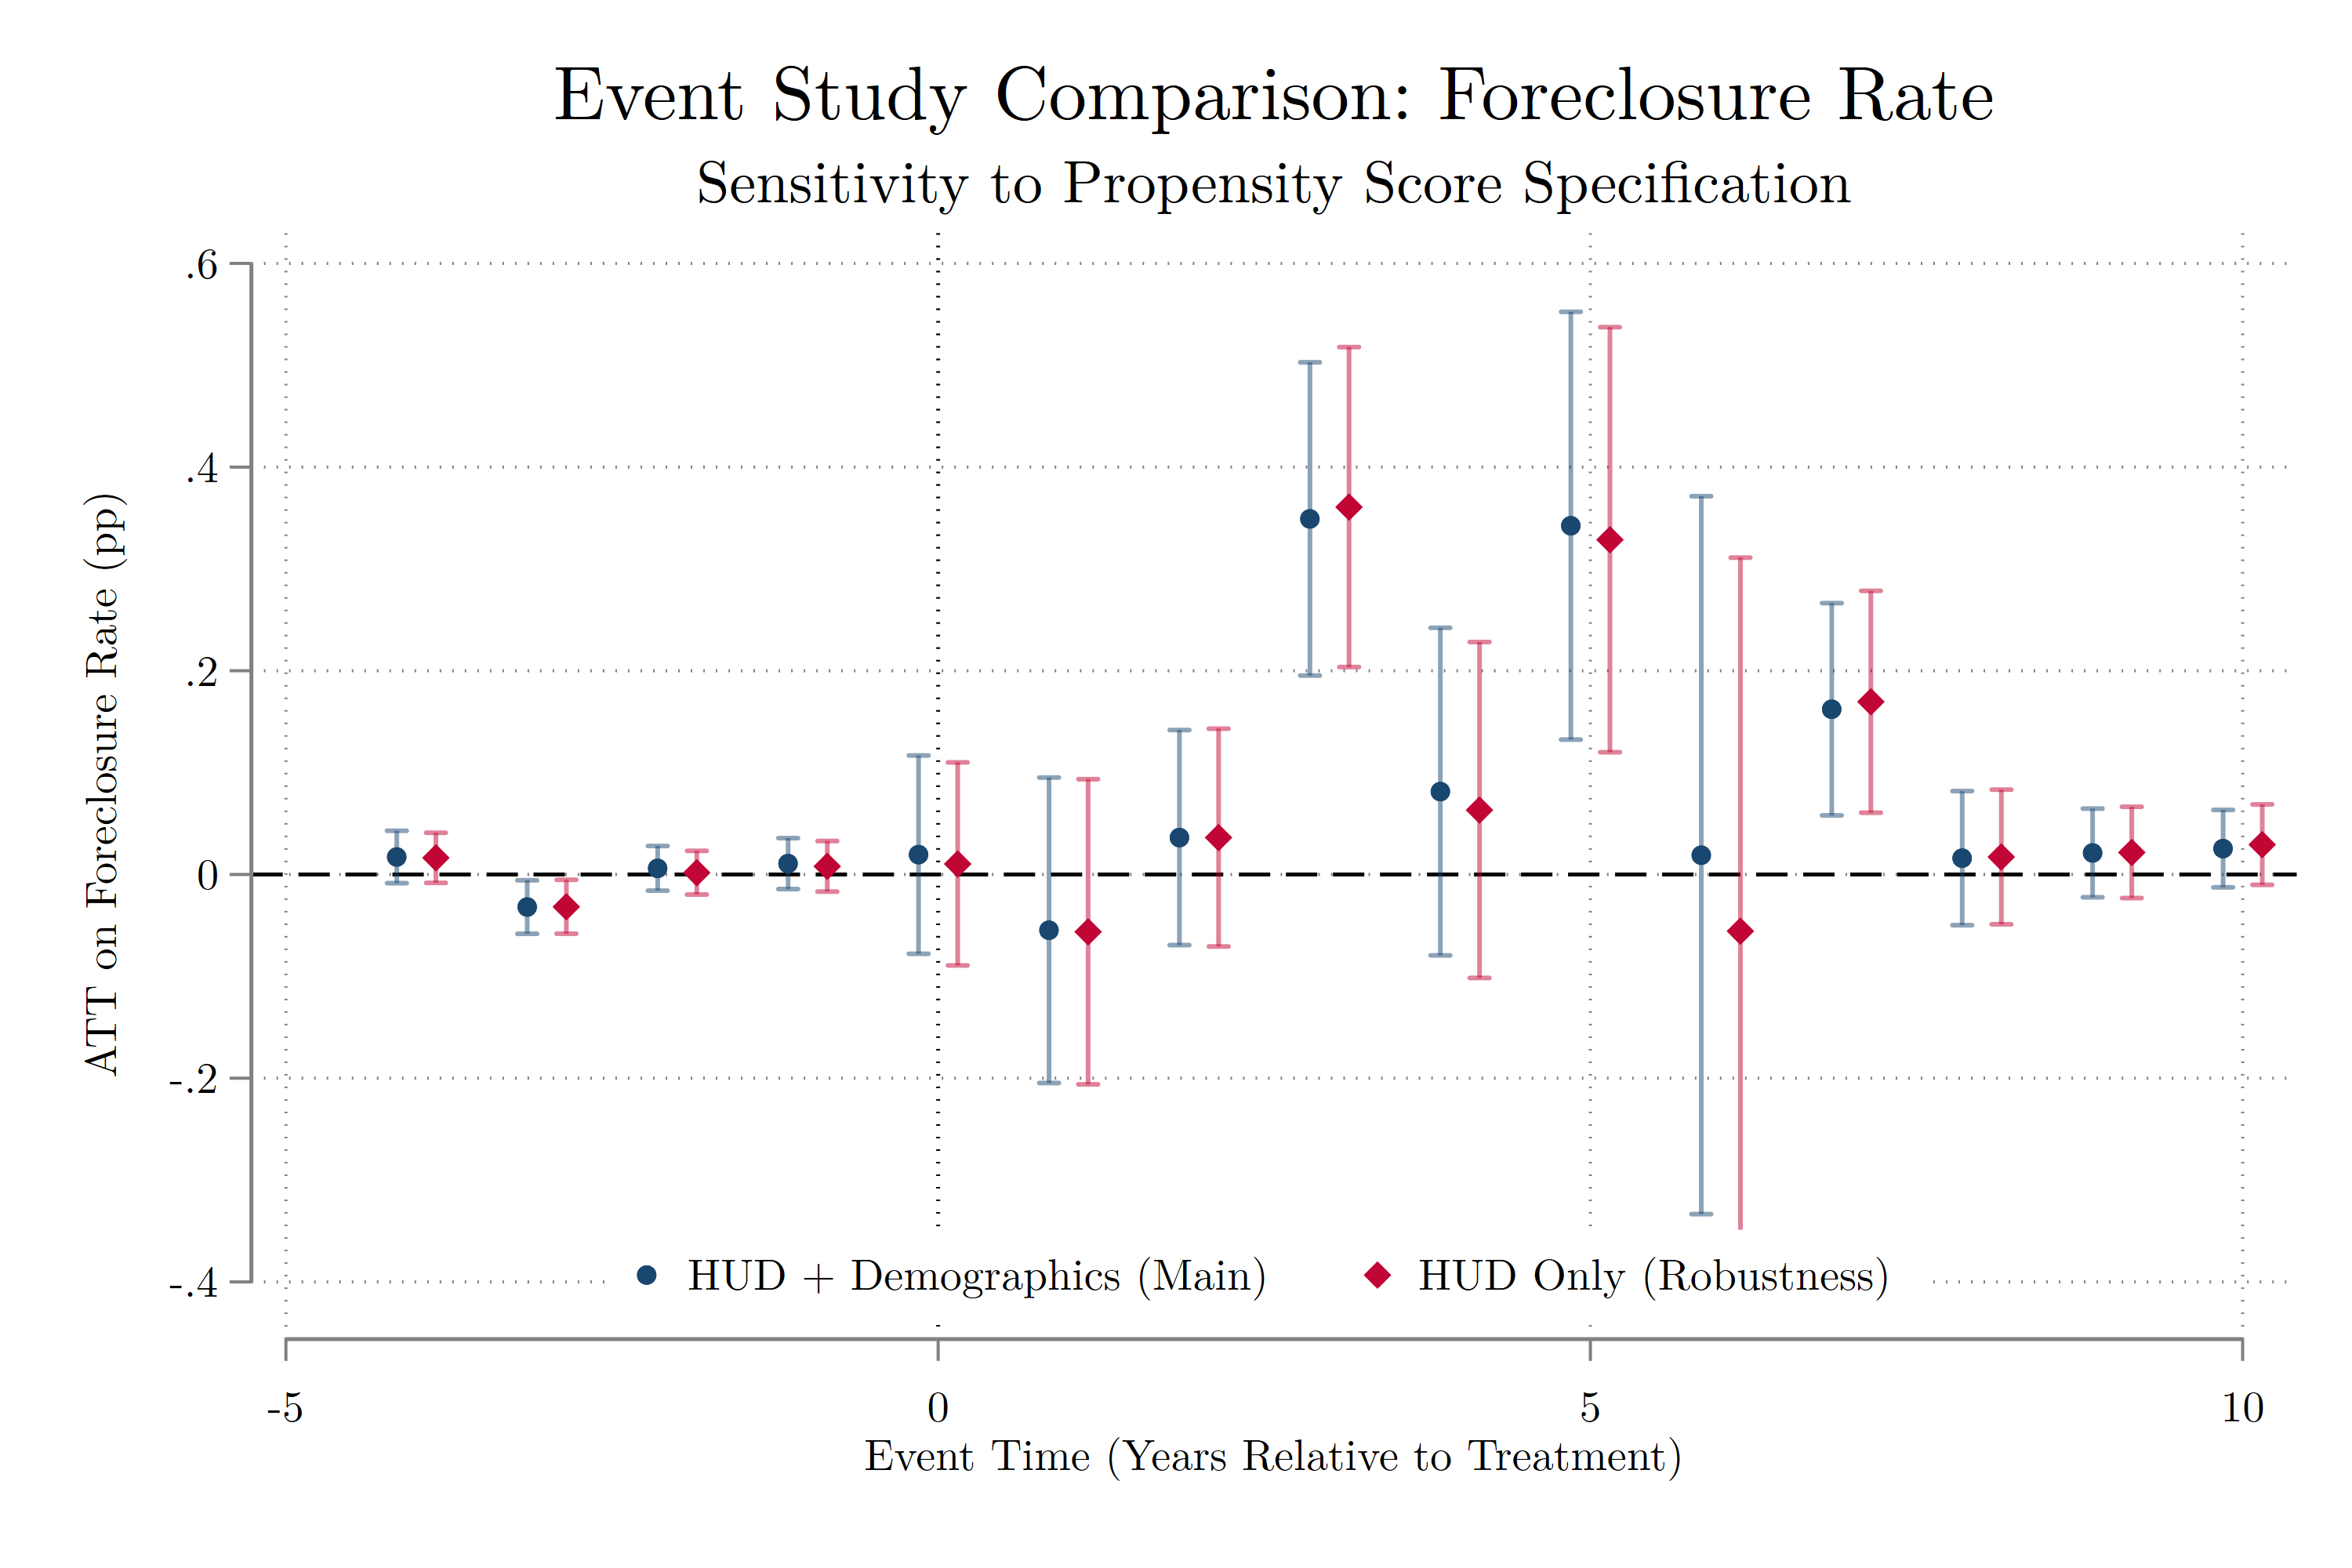
\includegraphics[width=0.85\textwidth]{cs_compare_specs_fore.png}
\caption{Event Study Comparison: Foreclosure Rate --- Sensitivity to Propensity Score Specification}
\label{fig:sensitivity_fore}
\begin{minipage}{\textwidth}
\footnotesize
\textit{Source:} Authors' calculations. \textit{Note:} Event study coefficients from the \citet{callaway2021} estimator with two propensity score specifications. 95\% confidence intervals shown.
\end{minipage}
\end{figure}

\subsection{Heterogeneity by Treatment Cohort}
\label{subsec:heterogeneity}

A key advantage of the staggered design is the ability to decompose the overall ATT into cohort-specific effects. Table~\ref{tab:cohort_results} and Figure~\ref{fig:cohort_atts} present the group-specific ATTs for NSP1 ($g = 2009$, $N = 599$) and NSP3 ($g = 2011$, $N = 68$).

The cohort-specific estimates reveal striking heterogeneity. For log sale prices, NSP1 shows a small and insignificant negative effect ($-0.039$, $p = 0.490$), while NSP3 shows a large and significant positive effect ($+0.217$, $p = 0.014$). For the foreclosure rate, the pattern reverses: NSP1 shows a borderline significant increase ($+0.099$, $p = 0.067$), while NSP3 shows no significant effect ($+0.037$, $p = 0.419$).

\begin{table}[htbp]
\centering
\caption{Cohort-Specific ATT Estimates: NSP1 (2009) vs.\ NSP3 (2011)}
\label{tab:cohort_results}
\begin{threeparttable}
\begin{tabular}{lcccc}
\toprule
& \multicolumn{2}{c}{ln(Sale Price)} & \multicolumn{2}{c}{Foreclosure Rate} \\
\cmidrule(lr){2-3} \cmidrule(lr){4-5}
& ATT & $p$-value & ATT & $p$-value \\
\midrule
NSP1 Cohort ($g = 2009$, $N = 599$) & $-0.039$ & $0.490$ & $+0.099^{*}$ & $0.067$ \\
& $(0.057)$ & & $(0.054)$ & \\
\addlinespace
NSP3 Cohort ($g = 2011$, $N = 68$) & $+0.217^{**}$ & $0.014$ & $+0.037$ & $0.419$ \\
& $(0.088)$ & & $(0.046)$ & \\
\bottomrule
\end{tabular}
\begin{tablenotes}[flushleft]
\footnotesize
\item \textit{Source:} Authors' calculations. \textit{Note:} Group-specific ATTs from the \citet{callaway2021} estimator with HUD + demographic controls. Standard errors in parentheses. $^{***} p < 0.01$, $^{**} p < 0.05$, $^{*} p < 0.10$.
\end{tablenotes}
\end{threeparttable}
\end{table}

\begin{figure}[htbp]
\centering
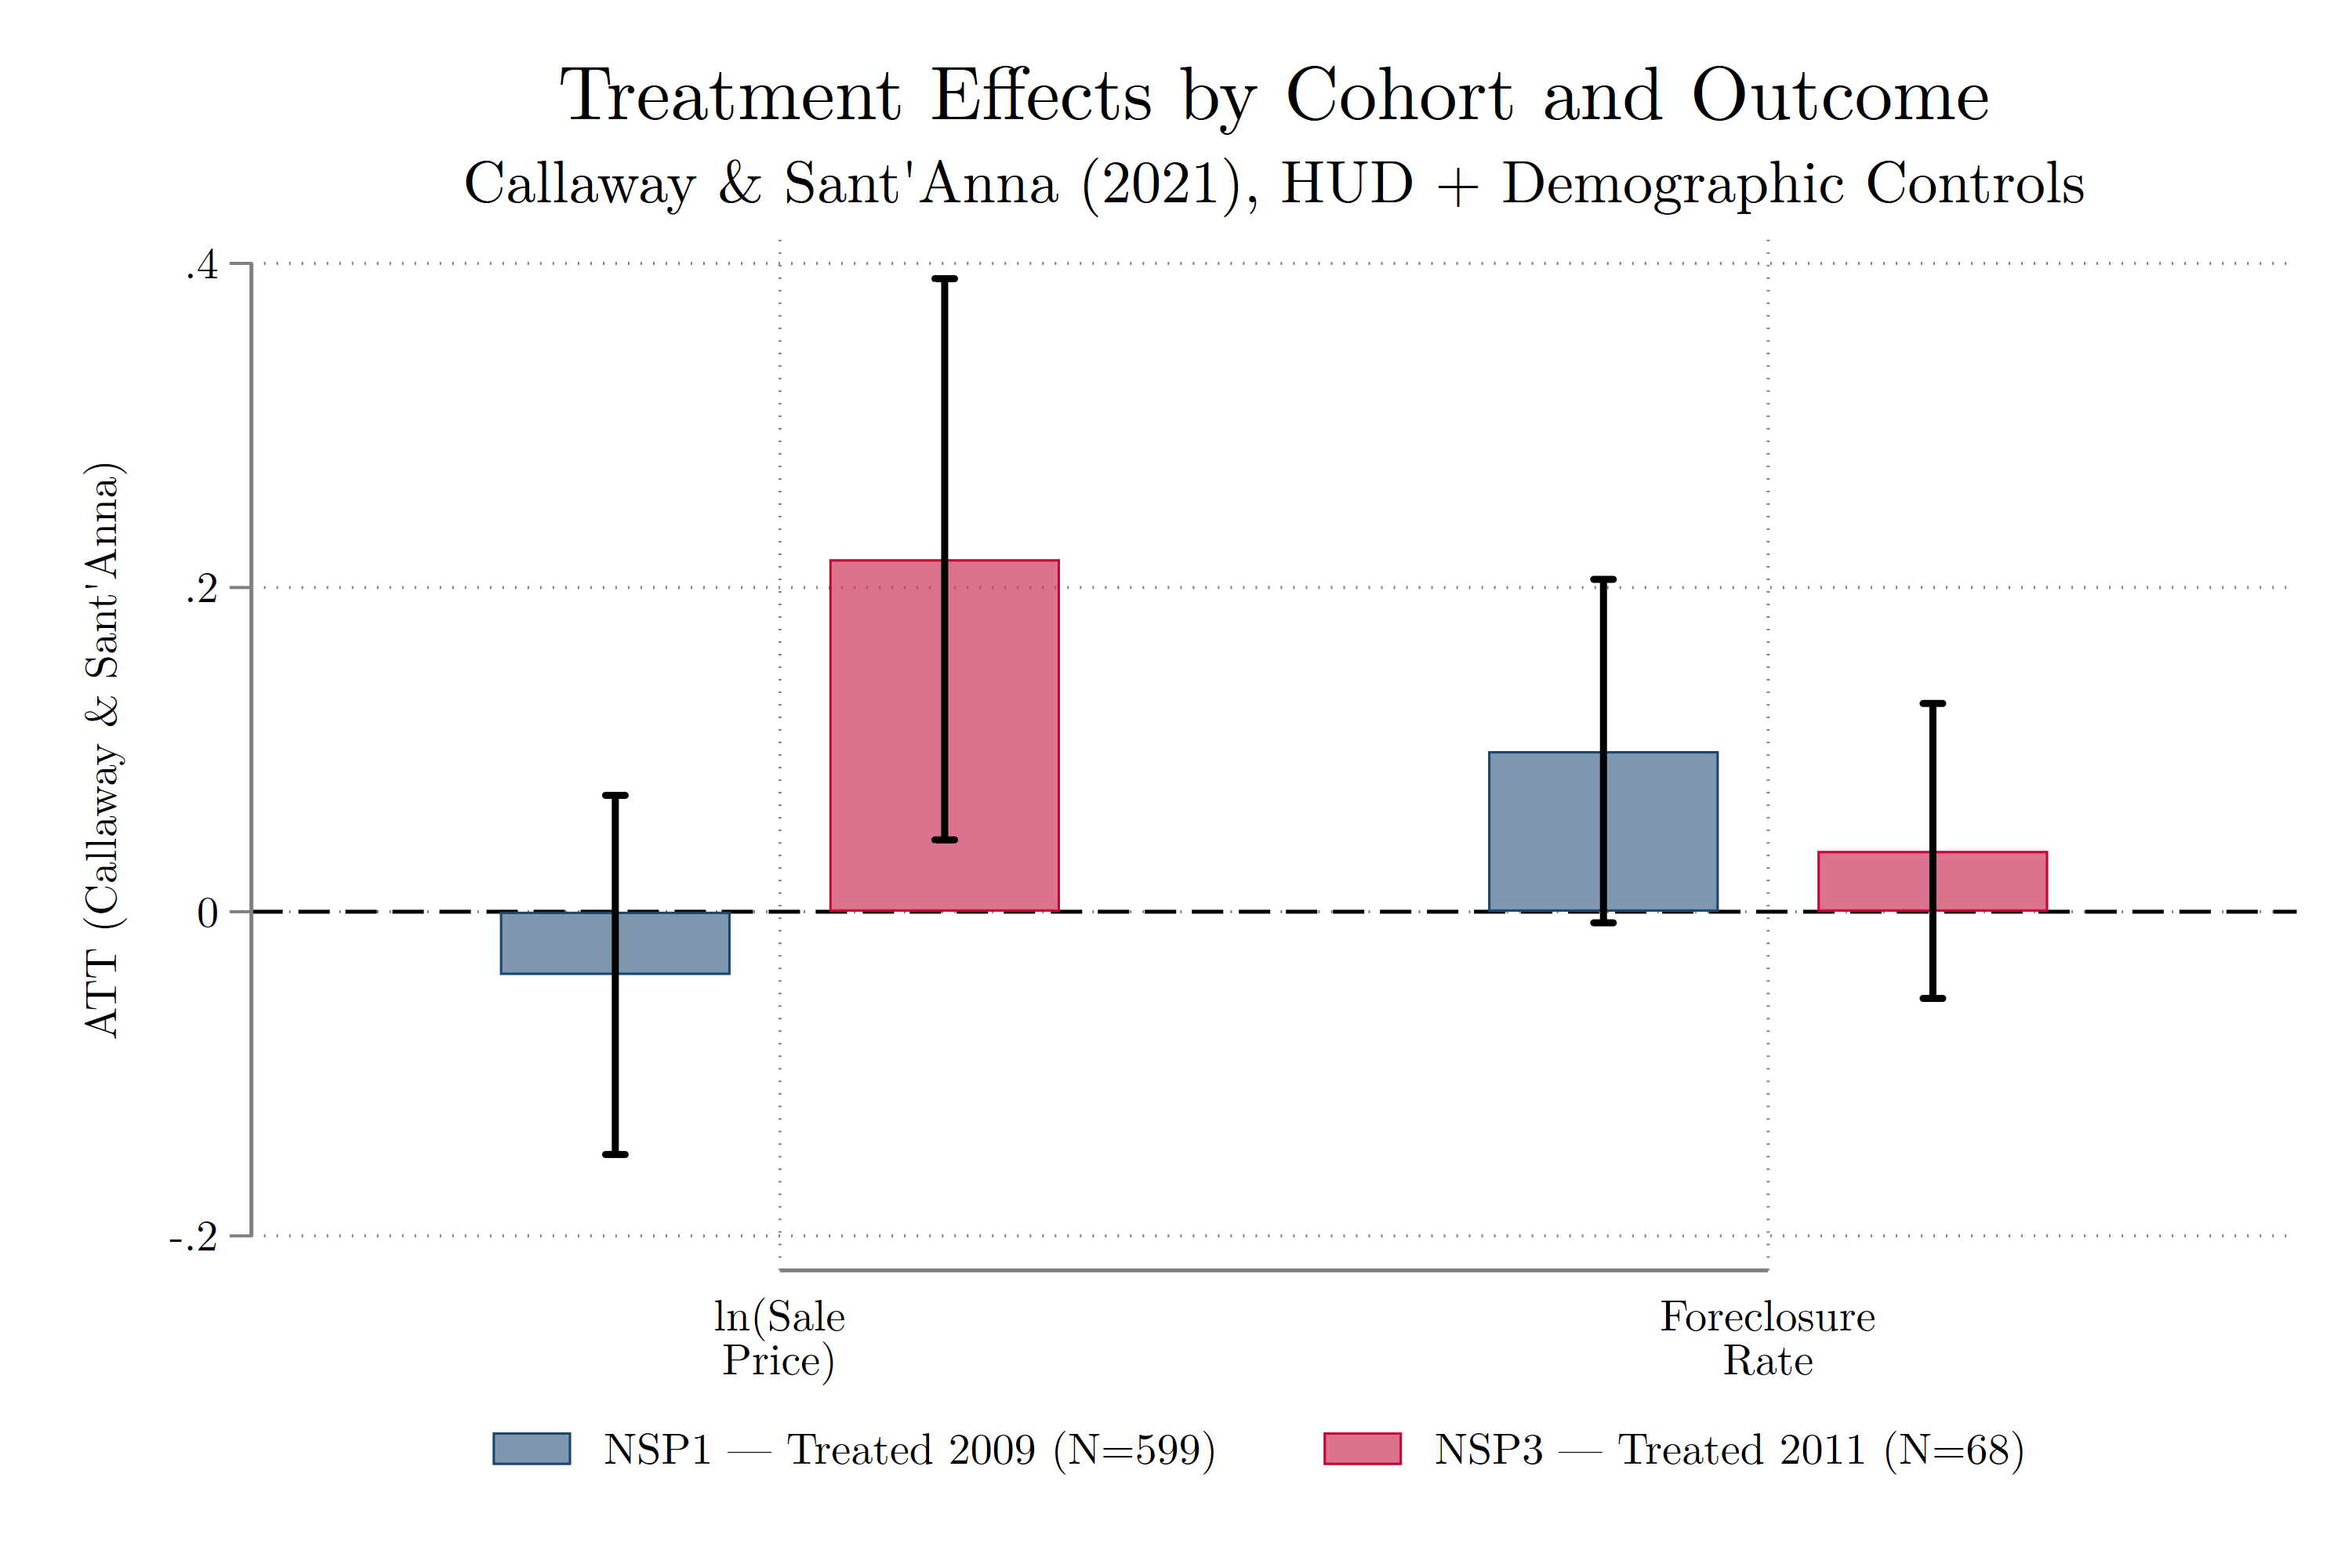
\includegraphics[width=0.85\textwidth]{cs_cohort_group_atts.png}
\caption{Cohort-Specific Group ATTs: NSP1 (2009) vs.\ NSP3 (2011)}
\label{fig:cohort_atts}
\begin{minipage}{\textwidth}
\footnotesize
\textit{Source:} Authors' calculations. \textit{Note:} Group-specific average treatment effects from the \citet{callaway2021} estimator with HUD + demographic controls. 95\% confidence intervals shown.
\end{minipage}
\end{figure}

These contrasting patterns have a coherent economic interpretation. NSP1 was deployed at the height of the foreclosure crisis in 2009, when Detroit's housing market was in freefall. The program targeted the most distressed neighborhoods at the worst possible moment---when the systemic forces driving price declines and foreclosure waves overwhelmed the modest stabilization resources available. In this context, the null price effect and the borderline foreclosure increase are consistent with the program being insufficient to counteract the crisis momentum.

NSP3, by contrast, was implemented in 2011, when markets had begun to stabilize. These areas, while still distressed, were less severely affected at baseline (Table~\ref{tab:summary}) and received treatment during a period of incipient recovery. The significant 21.7\% price increase for NSP3 areas suggests that the later round was able to leverage improving market conditions, consistent with the view that place-based interventions are most effective when complemented by broader economic recovery \citep{kline2013}.

\subsection{SUTVA Robustness: Addressing Spillover Effects}
\label{subsec:sutva}

A potential concern with our identification strategy is the violation of the Stable Unit Treatment Value Assumption (SUTVA). As Figure~\ref{fig:target_zones} illustrates, treated and control block groups in Detroit are spatially interleaved, with many control areas directly adjacent to treated zones. If the NSP generated positive (or negative) spillovers onto neighboring areas, the control group outcomes would be contaminated, biasing our estimates toward zero.

To address this concern, we re-estimate our main specification after dropping 101 control block groups that are directly adjacent to treated areas, leaving 298 non-adjacent controls. This SUTVA-robust sample eliminates the most plausible channel for spatial spillovers.

Table~\ref{tab:sutva_results} and Figures~\ref{fig:sutva_sale}--\ref{fig:sutva_fore} present the comparison between the full sample and the SUTVA-robust sample. For log sale prices, the results are virtually unchanged: the ATT moves from $-0.017$ ($p = 0.740$) to $-0.007$ ($p = 0.902$), remaining firmly insignificant. For the foreclosure rate, however, the SUTVA specification yields a notably stronger and now statistically significant result: the ATT increases from $+0.094$ ($p = 0.058$) to $+0.119$ ($p = 0.020$).

\begin{table}[htbp]
\centering
\caption{SUTVA Robustness: Dropping Adjacent Control Block Groups}
\label{tab:sutva_results}
\begin{threeparttable}
\begin{tabular}{lcccc}
\toprule
& \multicolumn{2}{c}{ln(Sale Price)} & \multicolumn{2}{c}{Foreclosure Rate} \\
\cmidrule(lr){2-3} \cmidrule(lr){4-5}
& ATT & $p$-value & ATT & $p$-value \\
\midrule
Full Sample ($N_{\text{control}} = 399$) & $-0.017$ & $0.740$ & $+0.094^{*}$ & $0.058$ \\
& $(0.053)$ & & $(0.049)$ & \\
\addlinespace
SUTVA ($N_{\text{control}} = 298$) & $-0.007$ & $0.902$ & $+0.119^{**}$ & $0.020$ \\
& $(0.057)$ & & $(0.051)$ & \\
\bottomrule
\end{tabular}
\begin{tablenotes}[flushleft]
\footnotesize
\item \textit{Source:} Authors' calculations. \textit{Note:} Both specifications use the \citet{callaway2021} estimator with HUD + demographic controls and staggered treatment timing. The SUTVA sample drops 101 control block groups adjacent to treated areas. Standard errors in parentheses. $^{***} p < 0.01$, $^{**} p < 0.05$, $^{*} p < 0.10$.
\end{tablenotes}
\end{threeparttable}
\end{table}

\begin{figure}[htbp]
\centering
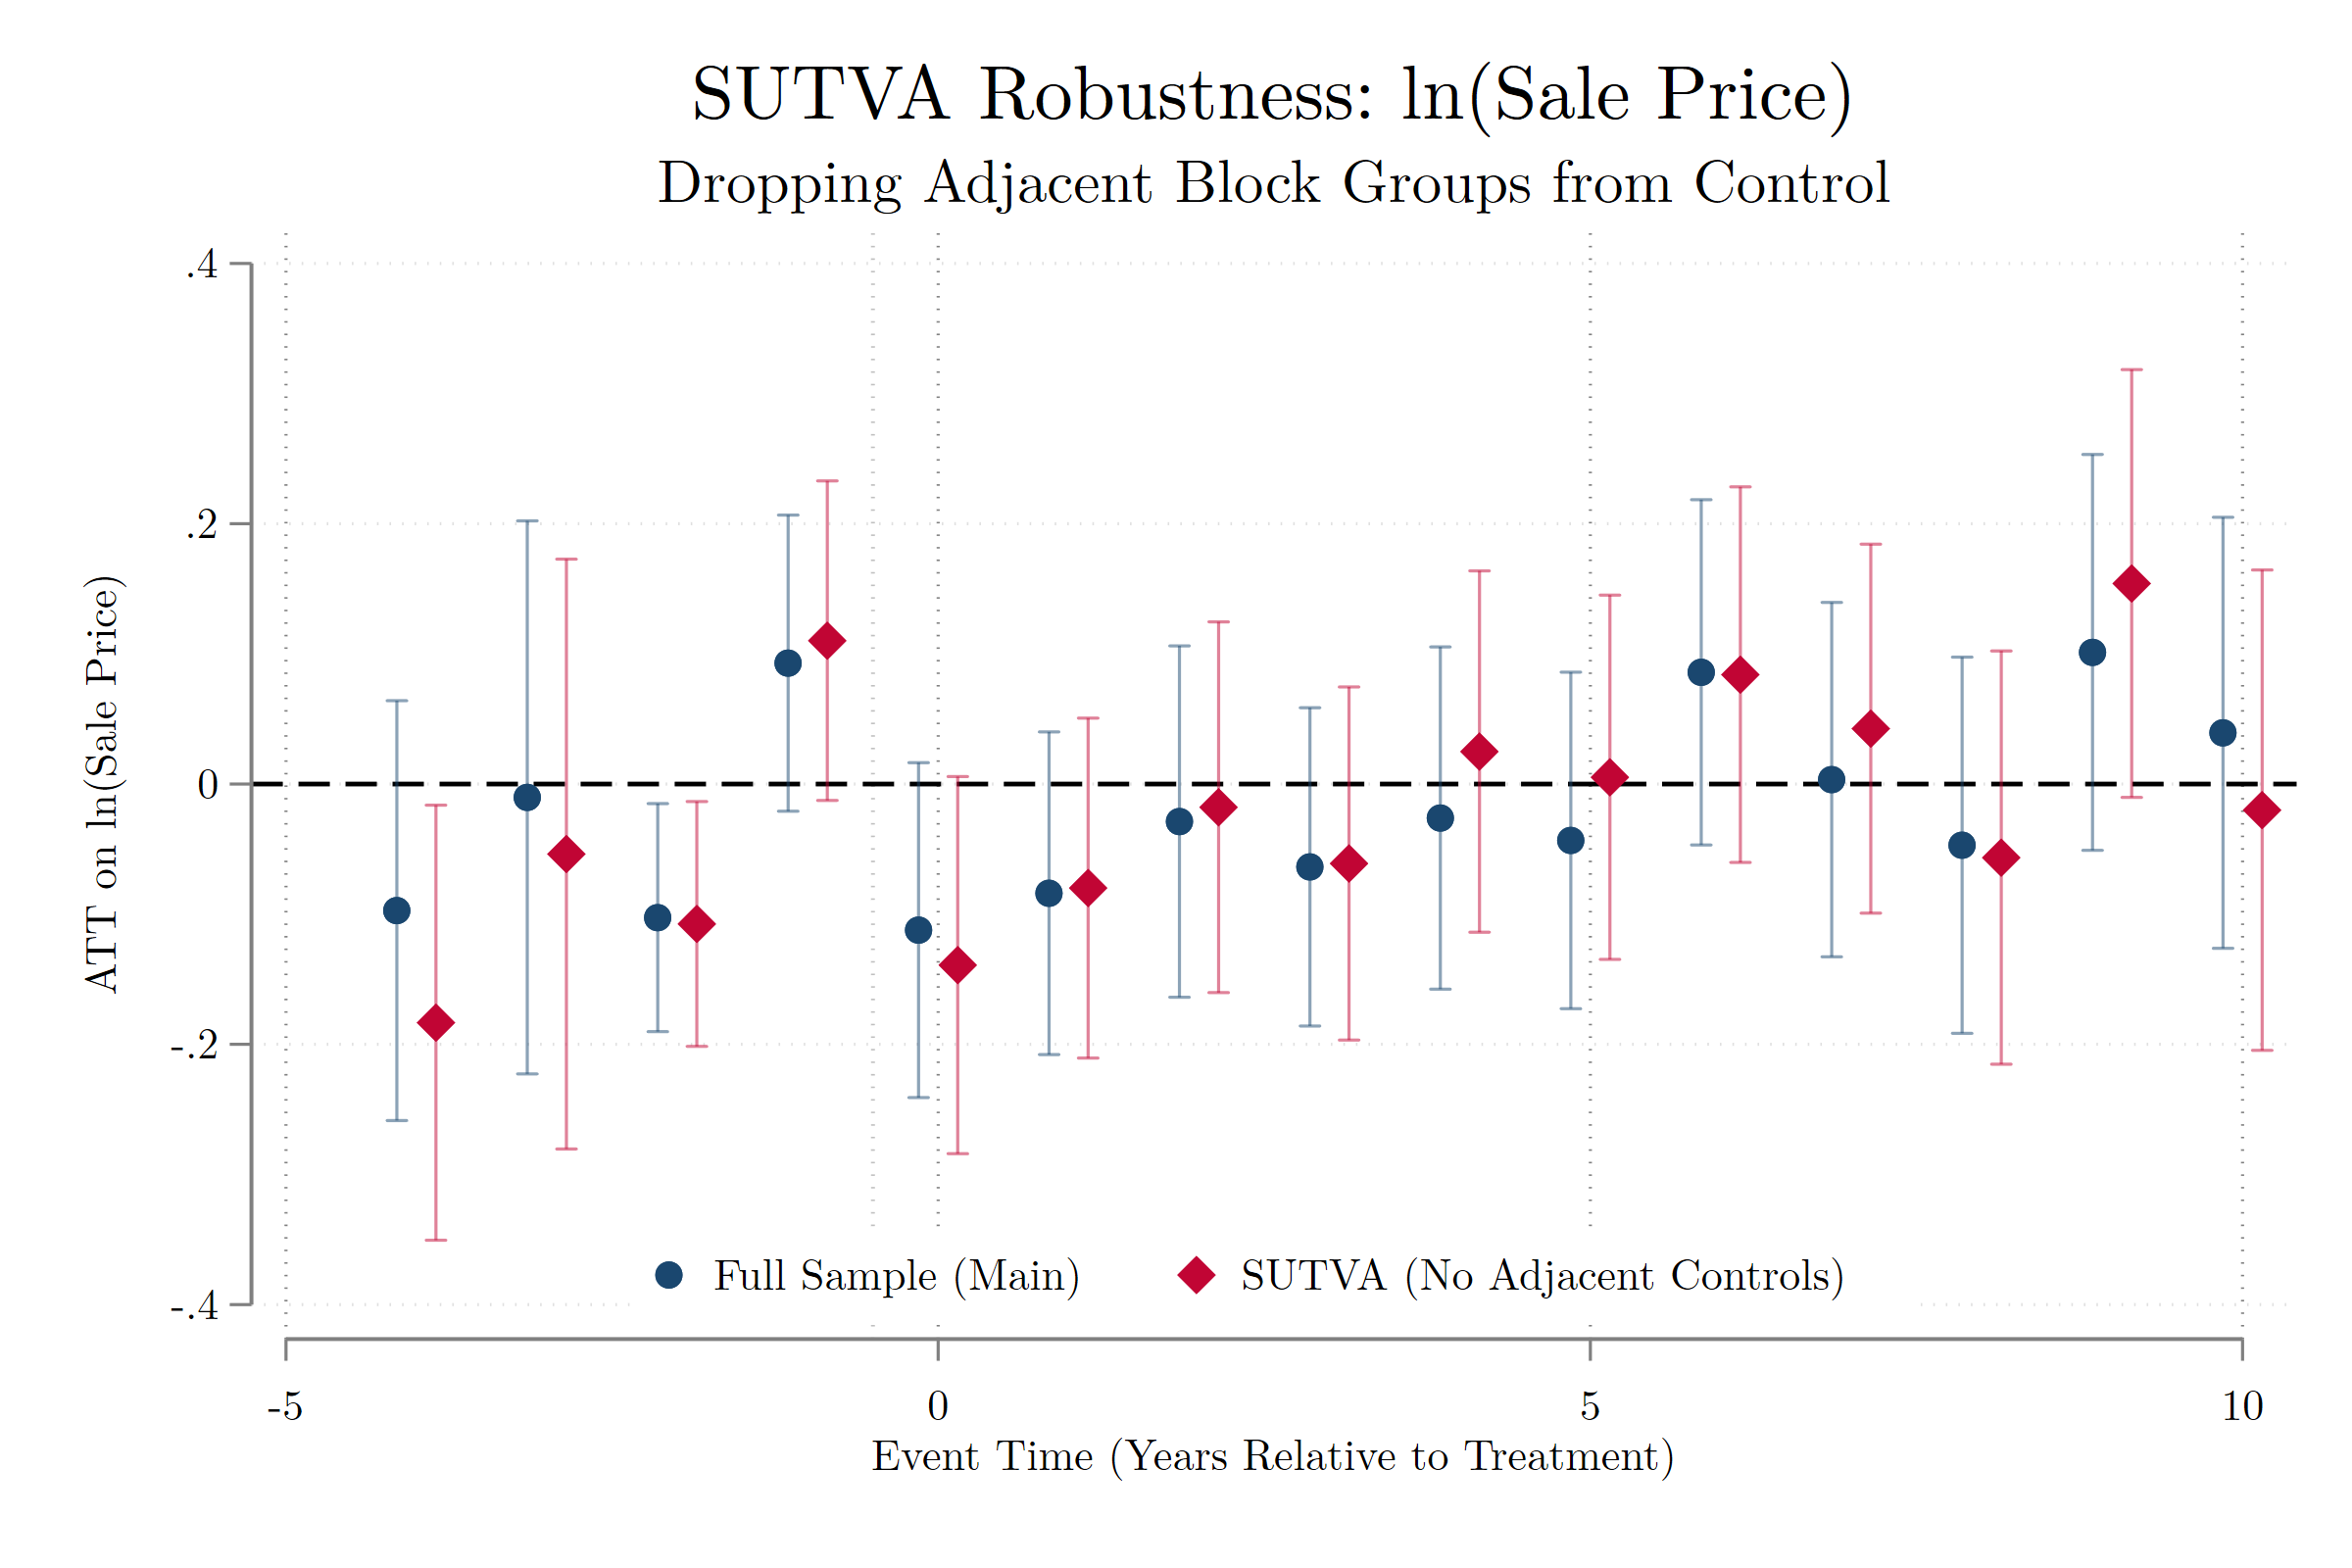
\includegraphics[width=0.85\textwidth]{sutva_compare_sale.png}
\caption{SUTVA Robustness: Event Study for ln(Sale Price)}
\label{fig:sutva_sale}
\begin{minipage}{\textwidth}
\footnotesize
\textit{Source:} Authors' calculations. \textit{Note:} Event study comparison between the full sample (circles, navy) and the SUTVA-robust sample excluding adjacent controls (diamonds, red). 95\% confidence intervals shown.
\end{minipage}
\end{figure}

\begin{figure}[htbp]
\centering
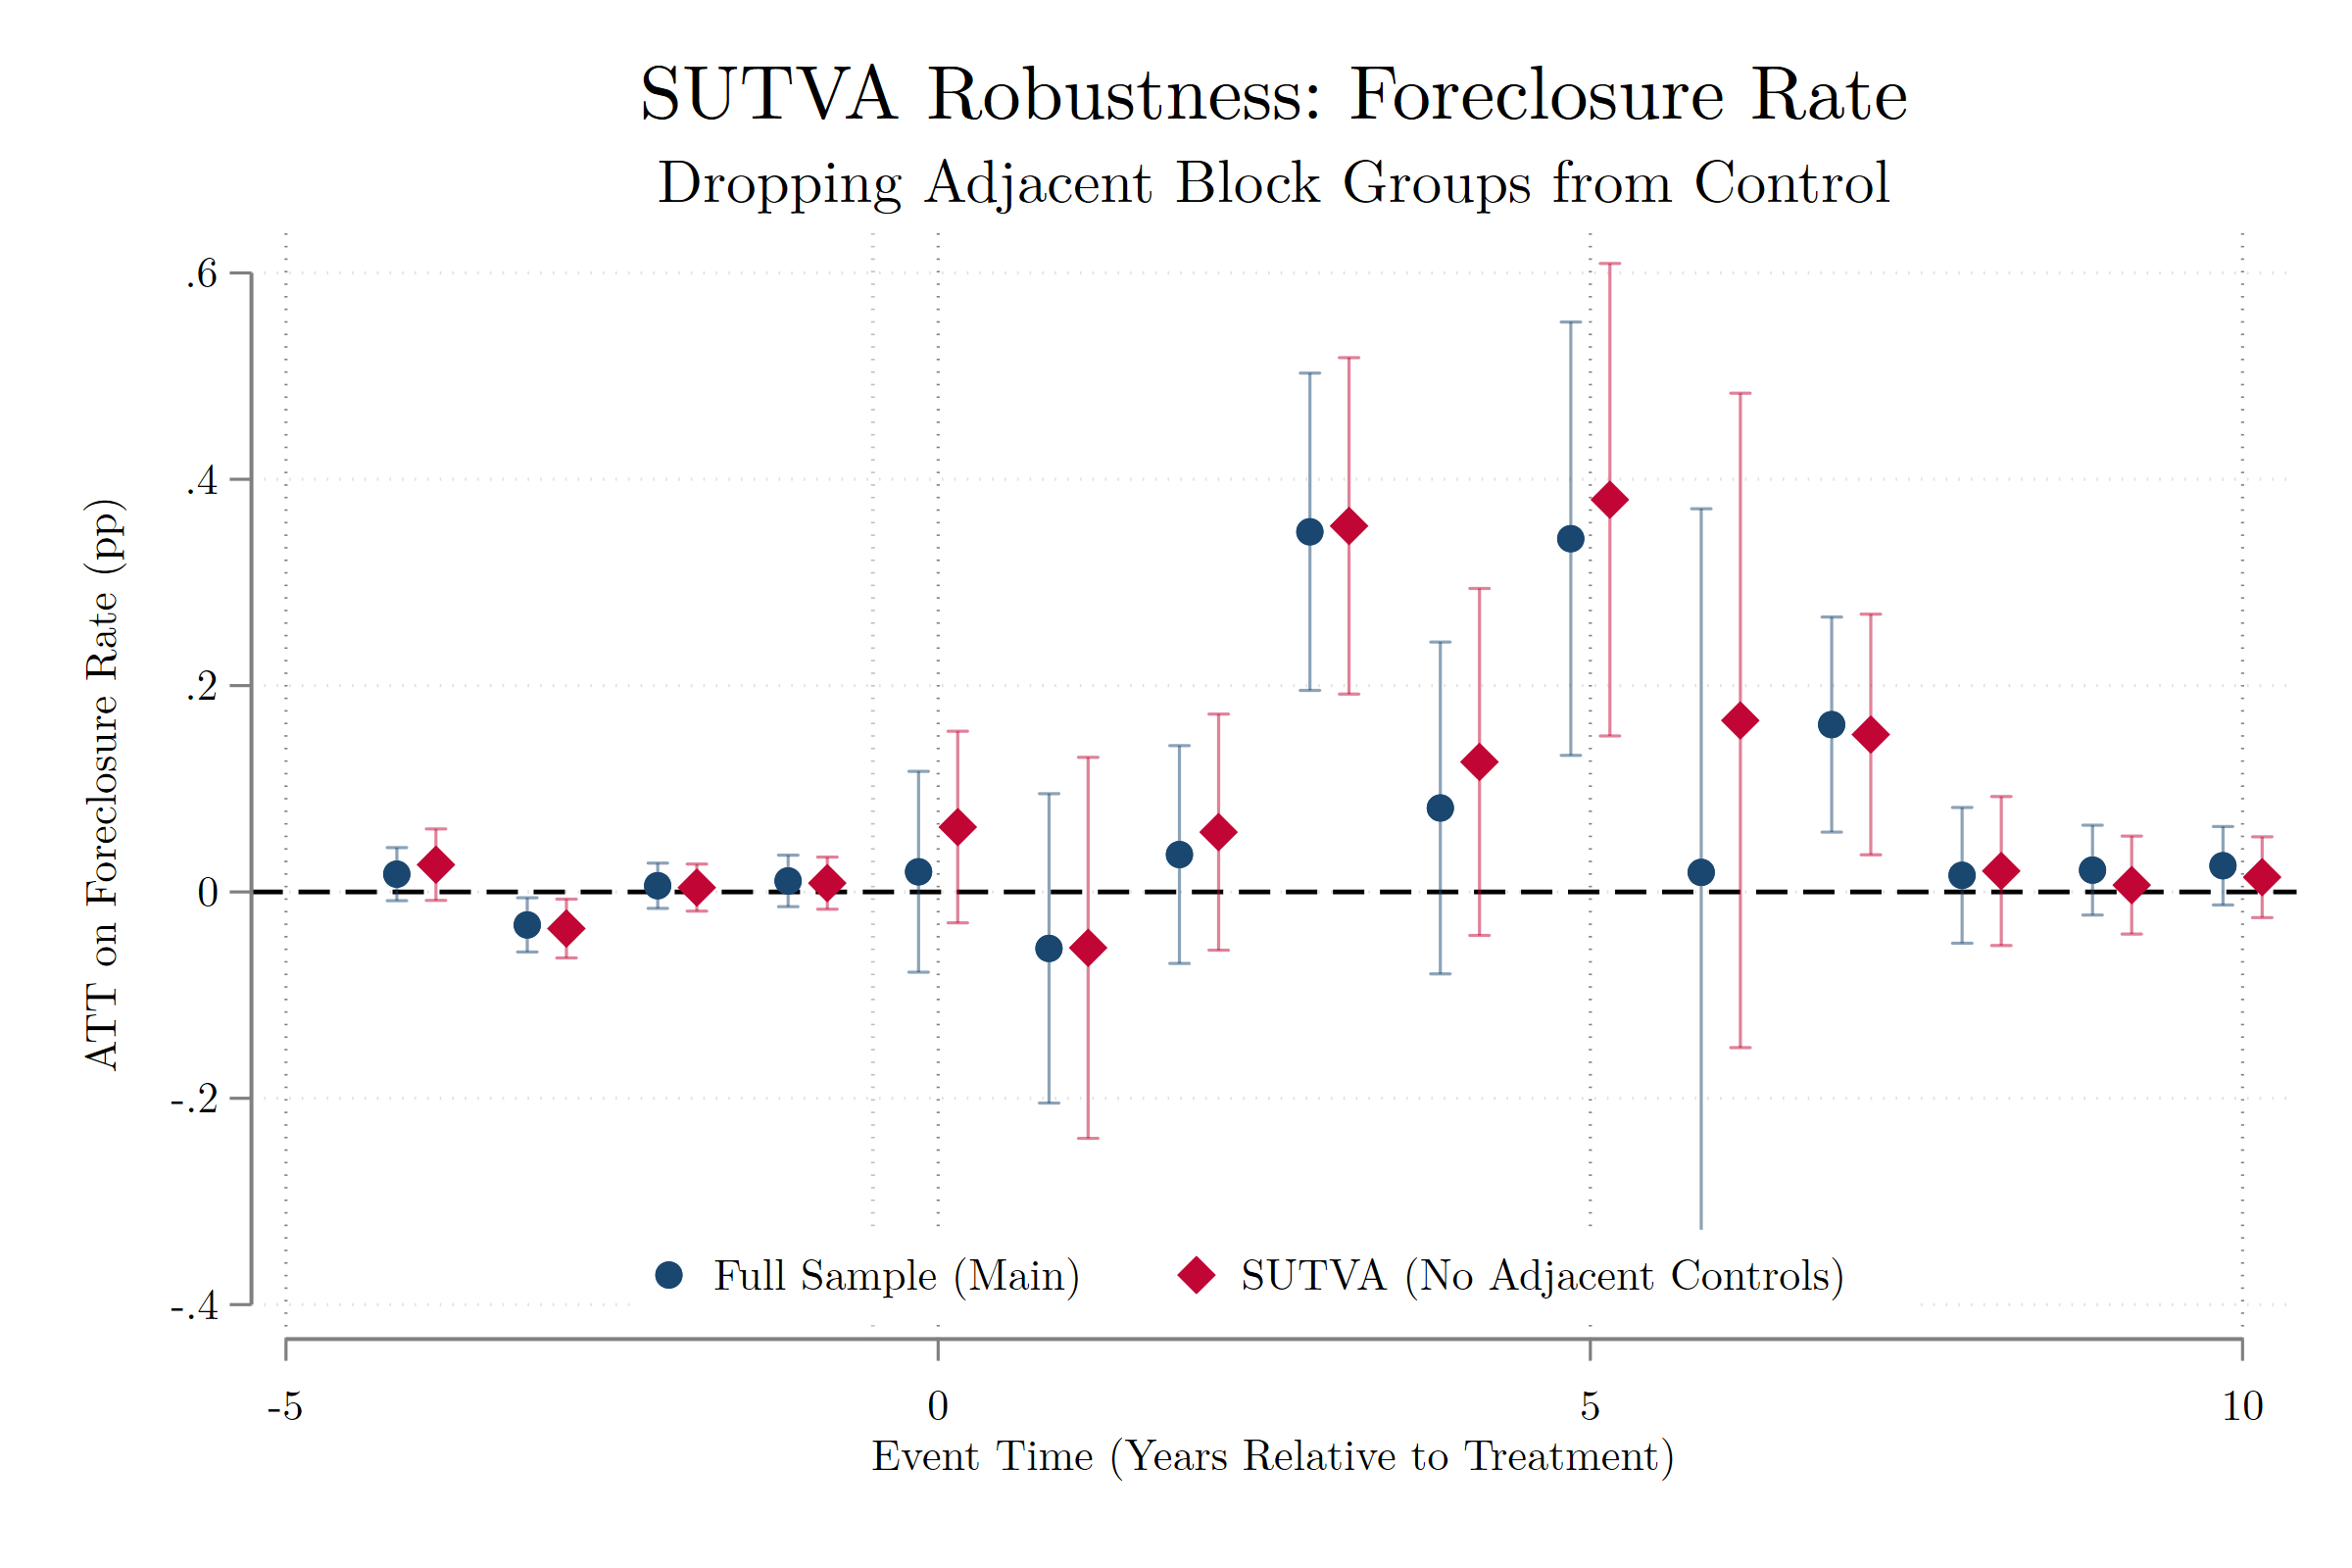
\includegraphics[width=0.85\textwidth]{sutva_compare_fore.png}
\caption{SUTVA Robustness: Event Study for Foreclosure Rate}
\label{fig:sutva_fore}
\begin{minipage}{\textwidth}
\footnotesize
\textit{Source:} Authors' calculations. \textit{Note:} Event study comparison between the full sample and the SUTVA-robust sample. 95\% confidence intervals shown.
\end{minipage}
\end{figure}

This finding has a natural interpretation. Adjacent control block groups were partially ``treated'' by spillovers from NSP activity in neighboring zones---for example, through demolition of blighted structures that reduced visual disamenities, or through rehabilitation projects that attracted investment to the broader area. These positive spillovers would have improved outcomes in adjacent controls, making the treated-vs-control contrast smaller. By removing these contaminated controls, the SUTVA-robust estimate recovers a larger and more precisely estimated treatment effect for foreclosures. The fact that the price effect remains null even in the SUTVA specification reinforces the conclusion that the program did not generate measurable price improvements.

\subsection{Interpretation}

The results paint a nuanced picture of NSP effectiveness that depends on three dimensions: outcome, timing, and spatial context.

First, regarding \textit{selection}: the dramatic difference between controlled and uncontrolled estimates---particularly for foreclosure rates ($+0.094$ vs.\ $+0.224$)---confirms that the HUD formula variables effectively capture the selection mechanism. This finding has important implications for evaluating other place-based policies where targeting is driven by observable distress indicators \citep{ding2016}.

Second, regarding \textit{timing}: the cohort heterogeneity suggests that place-based interventions in housing markets are most effective when they coincide with improving macroeconomic conditions. NSP1's null-to-negative effects during the crisis contrast sharply with NSP3's significant positive price effects during the recovery, echoing the broader finding that the effectiveness of local interventions depends on the aggregate economic environment \citep{kline2013}.

Third, regarding \textit{spillovers}: the SUTVA analysis reveals that the full-sample foreclosure estimate is attenuated by spatial spillovers. The 11.9 percentage point increase in the SUTVA specification ($p = 0.020$) indicates that treated areas experienced genuinely higher foreclosure rates than distant controls, likely reflecting the continued unwinding of distressed mortgages in the most severely affected neighborhoods---an effect that the NSP was insufficient to offset.

Our finding that the NSP had limited causal effects on housing prices does not necessarily mean the program was ineffective. The program may have prevented further deterioration that would have occurred absent the intervention, and the program's benefits may have been localized to the immediate vicinity of specific projects, effects that are averaged away at the block group level. The scale of Detroit's housing crisis---with over 139,000 foreclosures and decades of population decline \citep{alm2014}---may have overwhelmed the relatively modest NSP resources. As \citet{glaeser2005} argue, the durable nature of housing means that declining cities face persistent oversupply, limiting the efficacy of demand-side interventions.


% =============================================================================
\section{Conclusions}
\label{sec:conclusion}
% =============================================================================

This study evaluated the impact of the Neighborhood Stabilization Program in Detroit, focusing on housing prices and foreclosure rates. Using the \citet{callaway2021} difference-in-differences estimator with staggered treatment adoption, our analysis reveals a nuanced picture of NSP effectiveness that depends on timing, outcome, and spatial context.

Our first key finding concerns selection bias. The apparent treatment effects of the NSP are substantially attenuated by the HUD formula variables that guided program targeting. Without controlling for predicted foreclosure rates, subprime loan rates, residential vacancy rates, and demographic characteristics, estimated effects appear large and significant. Once these selection variables are included, the overall effects become small and insignificant for housing prices (ATT $= -0.017$, $p = 0.740$) and marginally significant for foreclosure rates (ATT $= +0.094$, $p = 0.058$). This has important implications for the evaluation of other place-based policies where targeting is based on observable distress indicators \citep{ding2016}.

Our second key finding concerns the role of timing. The cohort-specific analysis reveals striking heterogeneity: NSP1 ($g = 2009$), deployed at the height of the crisis, shows null price effects and borderline increases in foreclosures, while NSP3 ($g = 2011$), implemented during the early recovery, shows a significant 21.7\% increase in sale prices ($p = 0.014$) and no effect on foreclosures. This pattern suggests that the effectiveness of place-based interventions in housing markets depends critically on the macroeconomic context at the time of implementation \citep{kline2013}.

Our third finding concerns spatial spillovers. By dropping adjacent control block groups that may have been contaminated by treatment spillovers, the foreclosure effect strengthens from borderline ($p = 0.058$) to clearly significant ($p = 0.020$). This suggests that the full-sample estimate is attenuated by positive spillovers onto neighboring areas, and that accounting for SUTVA violations reveals a genuine---albeit modest---increase in foreclosure rates in treated areas.

The foreclosure rate results deserve particular attention. The event study reveals an inverted-U pattern, with treated areas experiencing temporarily higher foreclosure rates during the medium term, followed by convergence toward control areas by 2017--2019. This pattern is consistent with the mechanics of the foreclosure crisis in Detroit, where the peak of tax foreclosures occurred with a lag relative to the initial mortgage foreclosure wave \citep{alm2014}. The NSP targeted areas with the highest foreclosure risk, and these areas continued to experience elevated foreclosures in the medium term regardless of the intervention.

Several limitations of our analysis should be noted. First, our block group-level analysis may mask important heterogeneity in treatment effects at finer spatial scales. NSP rehabilitation projects may have generated positive spillovers within their immediate vicinity that are diluted when averaged across entire block groups. Second, the NSP3 cohort comprises only 68 block groups, limiting the precision of cohort-specific estimates for this group. Third, our analysis cannot capture general equilibrium effects, such as changes in migration patterns or labor market outcomes, that may result from neighborhood improvement.

Despite these limitations, our analysis demonstrates the value of exploiting staggered program implementation to uncover heterogeneous treatment effects, and the importance of properly accounting for both selection mechanisms and spatial spillovers in the evaluation of place-based policies. As Detroit continues to combat blight through successor programs---including the Proposal N bond-funded demolition initiative---our findings suggest that the timing of intervention relative to the crisis cycle matters at least as much as the scale of resources deployed. The NSP's emphasis on demolition and rehabilitation addressed the physical manifestation of decline, and the later round's success suggests that such interventions can be effective when they complement, rather than fight against, broader market recovery.

\singlespacing

% =============================================================================
% Bibliography
% =============================================================================

\bibliography{references}


% =============================================================================
% Appendix
% =============================================================================

\clearpage
\appendix
\doublespacing

\section{NSP Fund Allocation}
\label{app:allocation}

\begin{figure}[H]
\centering
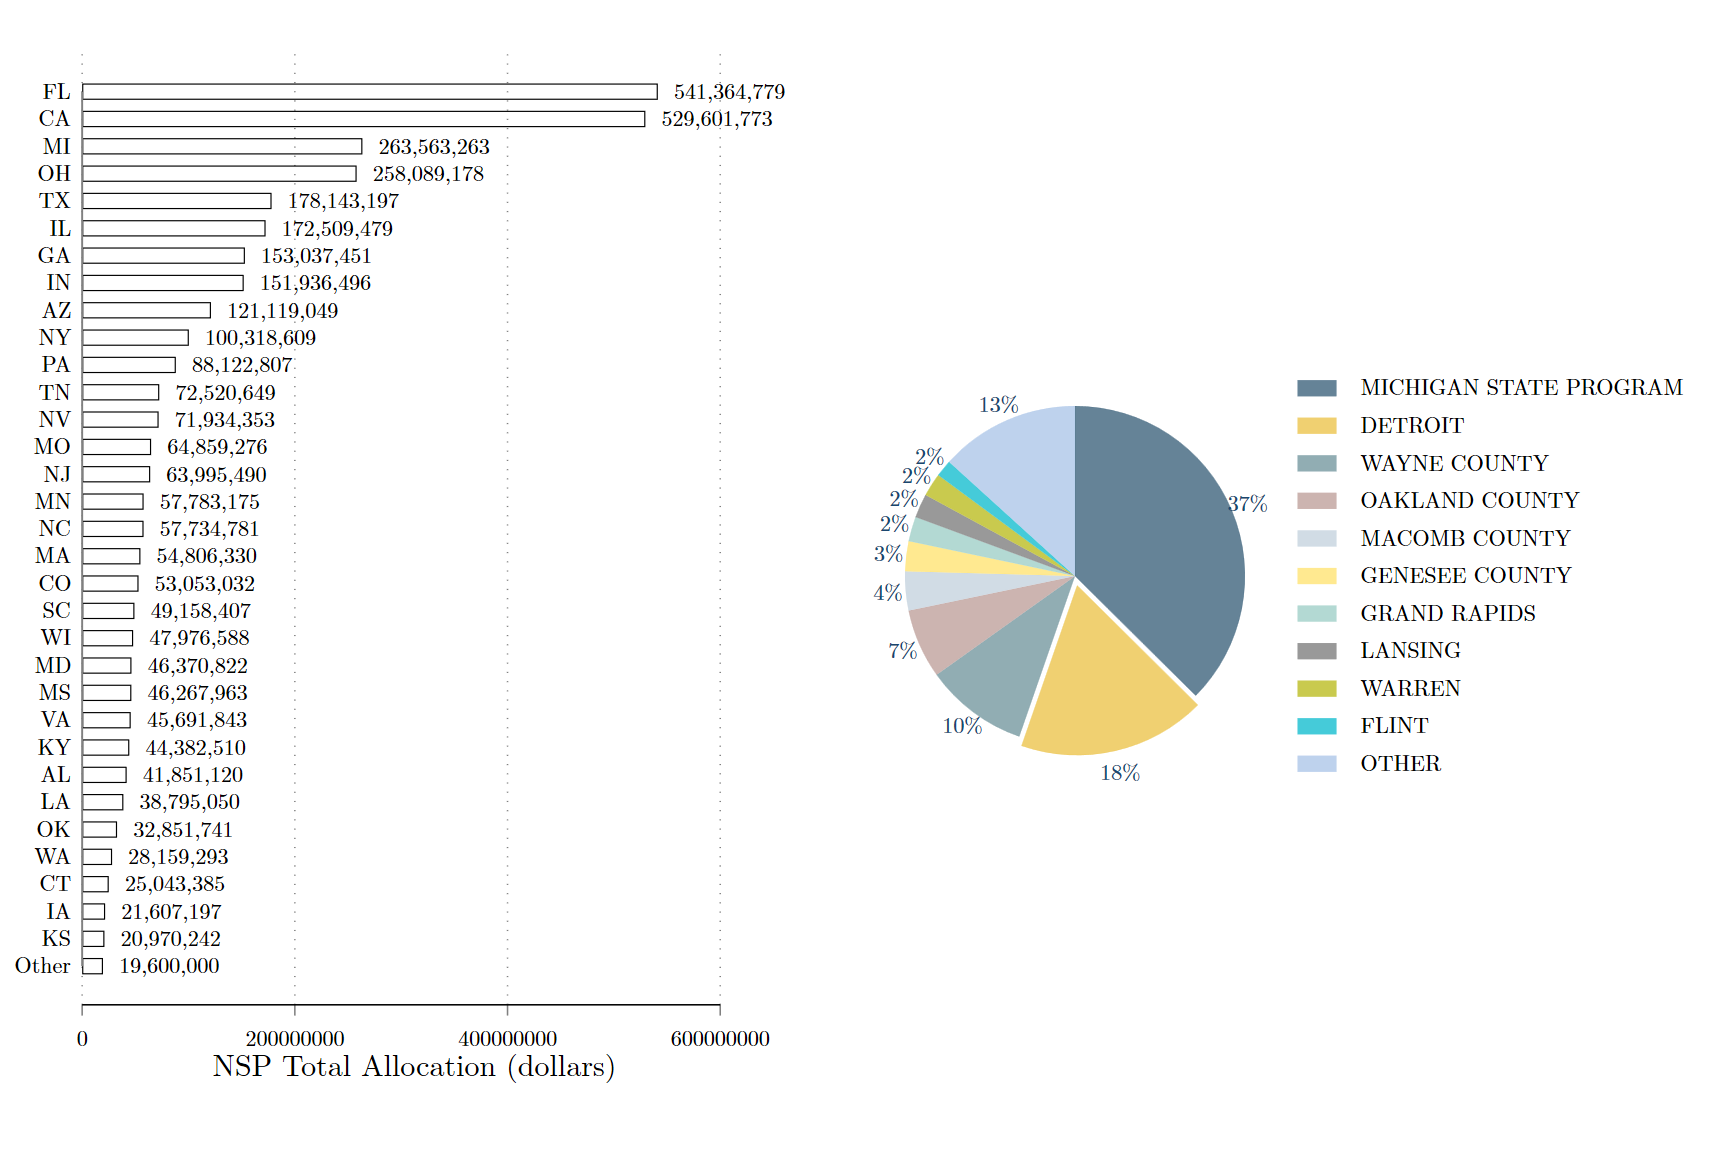
\includegraphics[width=0.85\textwidth]{nsp_allocation_states.png}
\caption{Allocation of NSP Funds at the State Level and Within the State of Michigan}
\label{fig:nsp_allocation}
\begin{minipage}{\textwidth}
\footnotesize
\textit{Source:} Authors' calculations using information from the United States Department of Housing and Urban Development (HUD). \textit{Note:} Bar chart presents the distribution of NSP funds from the first round by state. Michigan was the third-largest recipient. A pie chart showing the distribution within Michigan is presented to the right.
\end{minipage}
\end{figure}


\section{NSP Target Zone Selection Criteria}
\label{app:criteria}

\begin{table}[H]
\centering
\caption{Criteria for Defining NSP Target Zones in the City of Detroit}
\label{tab:selection_criteria}
\begin{threeparttable}
\small
\begin{tabularx}{\textwidth}{lX}
\toprule
Criteria & Description \\
\midrule
LMMH Area & Properties benefiting from NSP must be in low, moderate, and middle-income areas, where over 51\% of people have incomes less than 120\% of the Area Median Income. \\
\addlinespace
HUD Data & Properties must be in areas with: highest percentage of foreclosures; highest percentage of homes financed by subprime mortgage-related loans; identified as likely to face a significant rise in the rate of home foreclosures. \\
\addlinespace
Foreclosure Data & Properties must have high rates of mortgage foreclosures in 2006 and 2007. Adjusted by the city. \\
\addlinespace
Local Target Areas & Areas with high private sector investment (building permits), Block Grant activity, urban renewal activity, and federally designated Empowerment Zone activity. \\
\addlinespace
Citywide Policies & Areas congruent with citywide policies from the Master Plan. \\
\bottomrule
\end{tabularx}
\begin{tablenotes}[flushleft]
\footnotesize
\item \textit{Source:} Authors' elaboration based on ``Neighborhood Stabilization Plan'' by the Planning and Development Department of the City of Detroit \citep{pdd2009}.
\end{tablenotes}
\end{threeparttable}
\end{table}


\section{Additional Robustness: AIPW and TWFE Estimates}
\label{app:robustness}

We complement the Callaway and Sant'Anna estimates with two additional approaches. The augmented inverse probability weighting (AIPW) estimator \citep{wooldridge2023} incorporates a richer set of covariates including distance to CBD with a quadratic term. The traditional two-way fixed effects (TWFE) estimator serves as a benchmark, noting that in our staggered setting the TWFE bias documented by \citet{goodmanbacon2021} may be present. Results are presented in Table~\ref{tab:robustness_appendix}.

\begin{table}[H]
\centering
\caption{Robustness: AIPW and TWFE Estimates}
\label{tab:robustness_appendix}
\begin{threeparttable}
\small
\begin{tabular}{lcccccc}
\toprule
& \multicolumn{2}{c}{AIPW (Wooldridge)} & \multicolumn{2}{c}{TWFE (no controls)} & \multicolumn{2}{c}{TWFE (HUD controls)} \\
\cmidrule(lr){2-3} \cmidrule(lr){4-5} \cmidrule(lr){6-7}
& ln(Price) & Fore.\ Rate & ln(Price) & Fore.\ Rate & ln(Price) & Fore.\ Rate \\
\midrule
ATT & $-0.027$ & $+0.100$ & $-0.126$ & $+0.241$ & $-0.008$ & $+0.095$ \\
& $(0.003)$ & $(0.004)$ & $(0.038)$ & $(0.046)$ & $(0.031)$ & $(0.040)$ \\
$p$-value & $<0.001$ & $<0.001$ & $0.001$ & $<0.001$ & $0.802$ & $0.018$ \\
\bottomrule
\end{tabular}
\begin{tablenotes}[flushleft]
\footnotesize
\item \textit{Source:} Authors' calculations. \textit{Note:} AIPW: \citet{wooldridge2023} with HUD formula variables, demographic controls, and distance to CBD. TWFE: block group and year fixed effects; HUD controls interacted with year dummies where indicated. $^{***} p < 0.01$, $^{**} p < 0.05$, $^{*} p < 0.10$.
\end{tablenotes}
\end{threeparttable}
\end{table}

\section{Cohort-Specific Event Studies}
\label{app:cohort_events}

Figures~\ref{fig:cohort_event_sale} and \ref{fig:cohort_event_fore} present the cohort-specific event study plots, which decompose the aggregated event studies into separate trajectories for NSP1 ($g = 2009$) and NSP3 ($g = 2011$).

\begin{figure}[H]
\centering
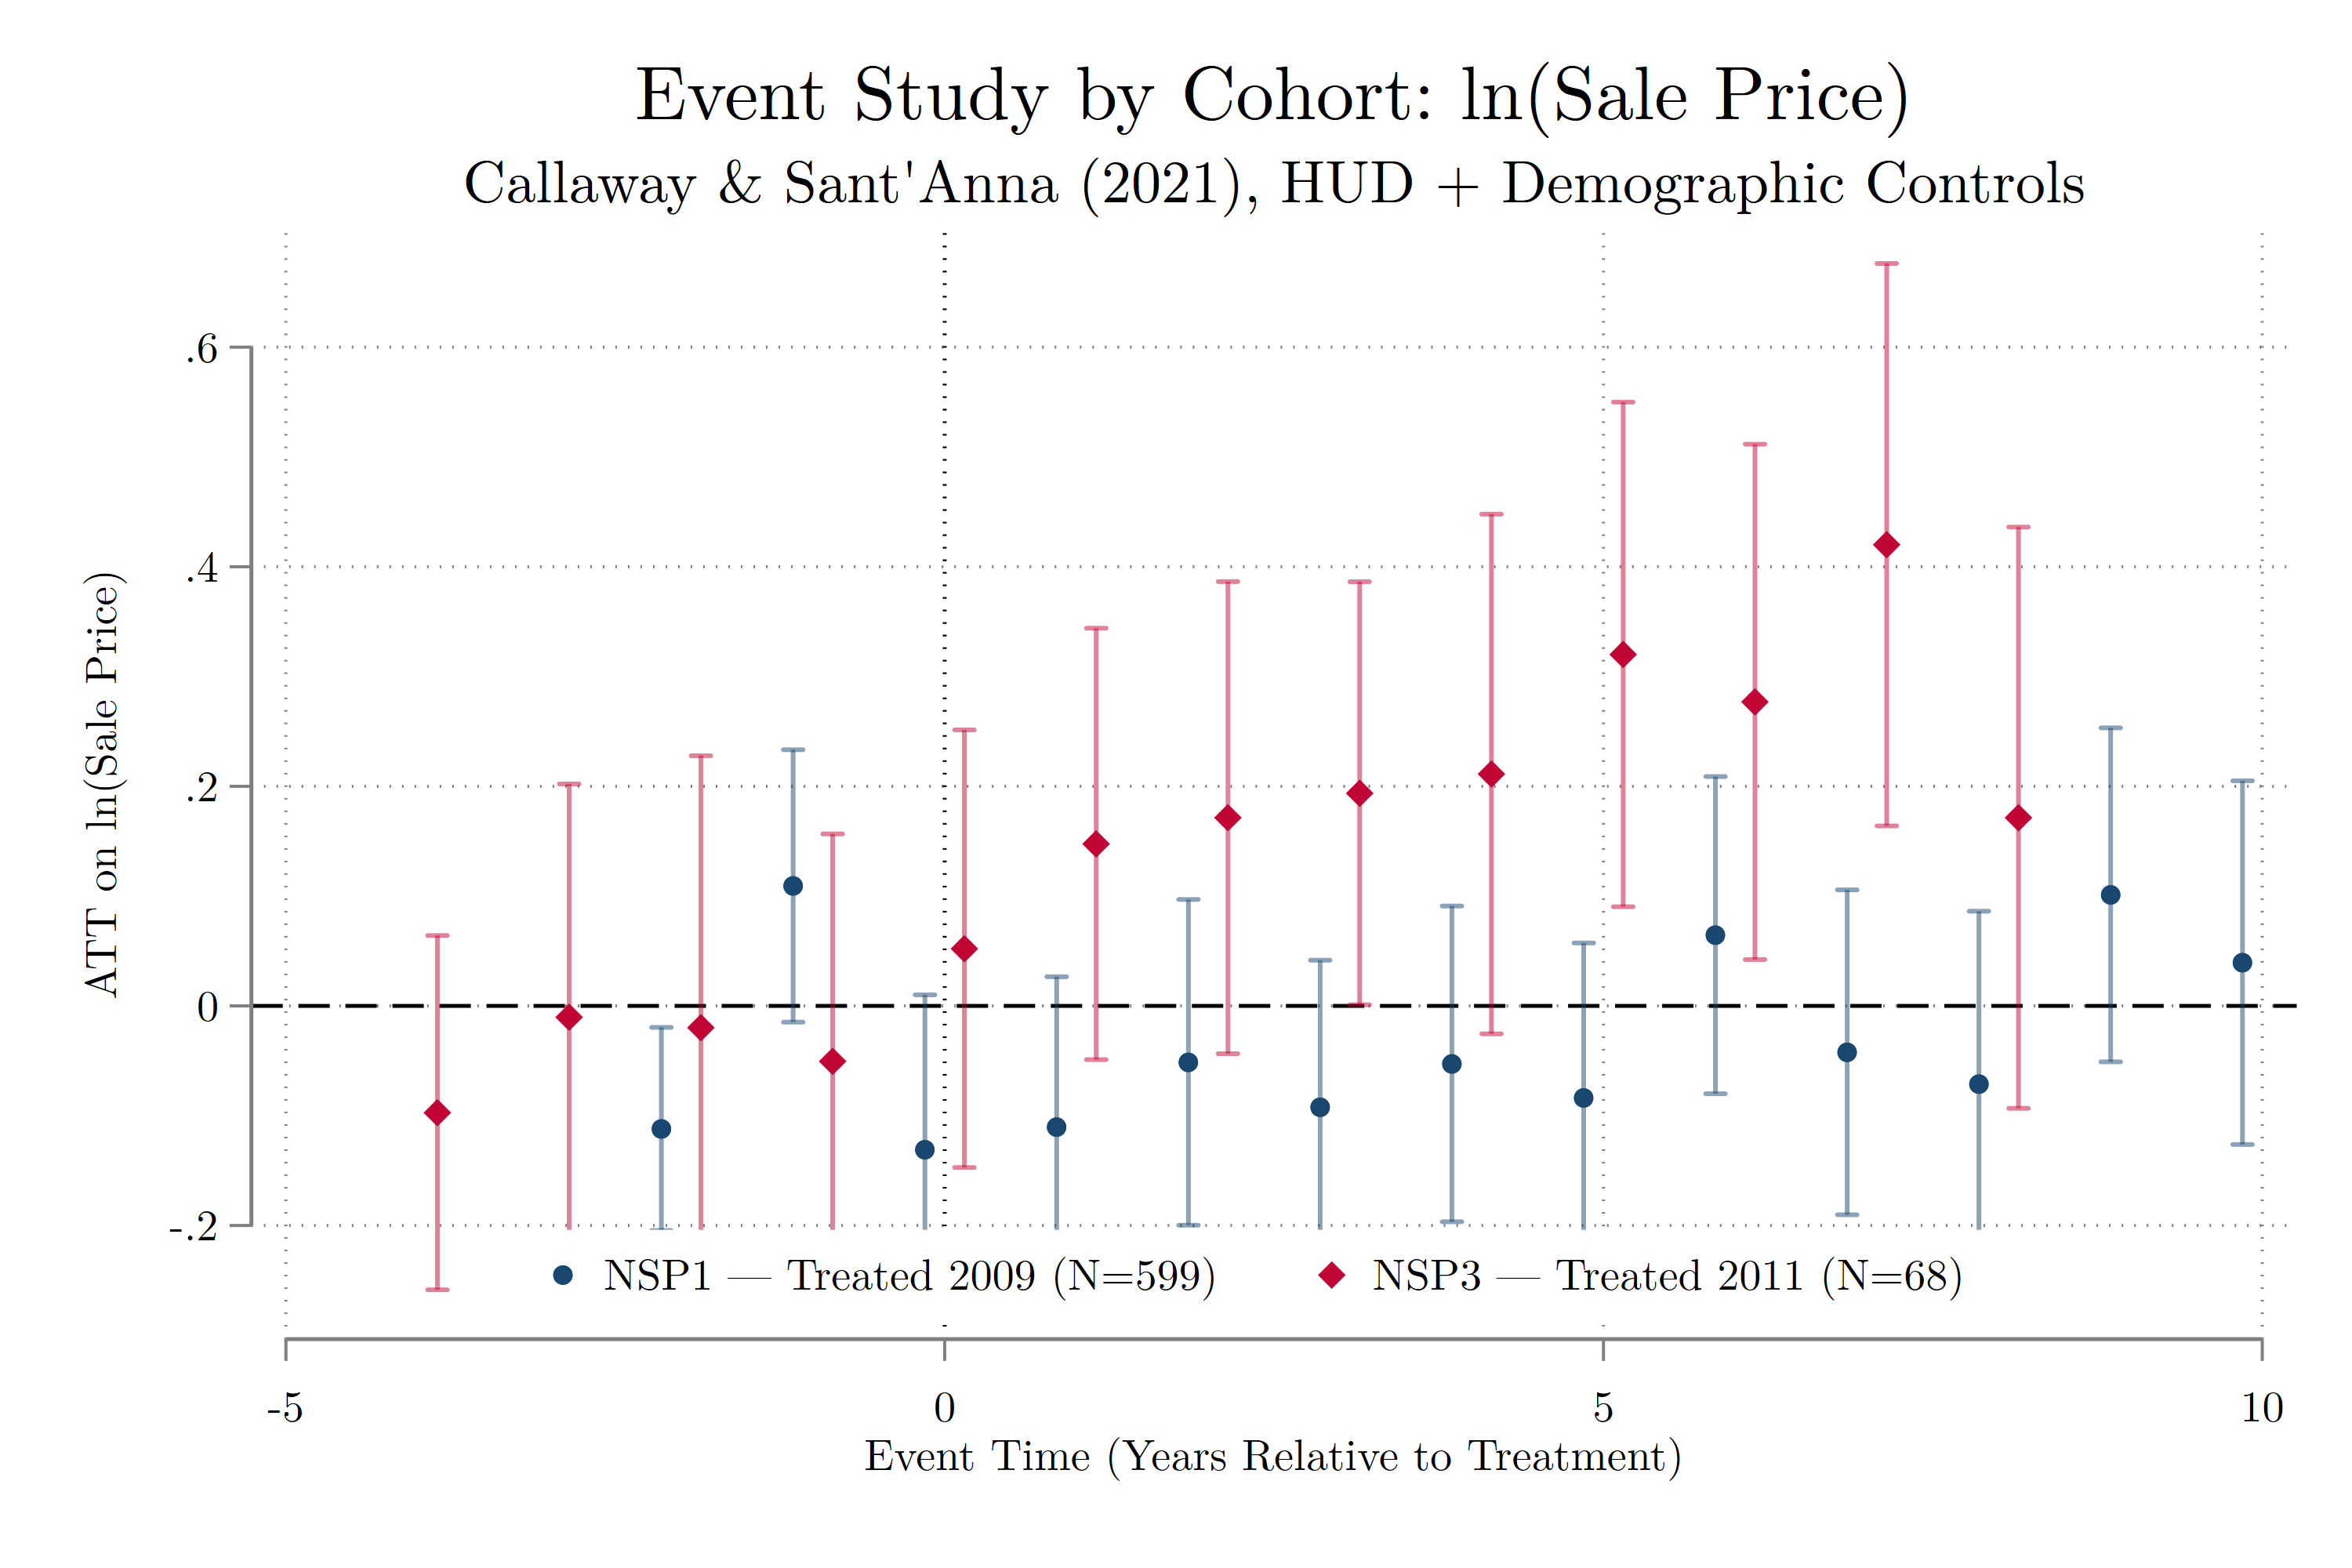
\includegraphics[width=0.85\textwidth]{cs_cohort_sale_event.png}
\caption{Cohort-Specific Event Study: ln(Sale Price)}
\label{fig:cohort_event_sale}
\end{figure}

\begin{figure}[H]
\centering
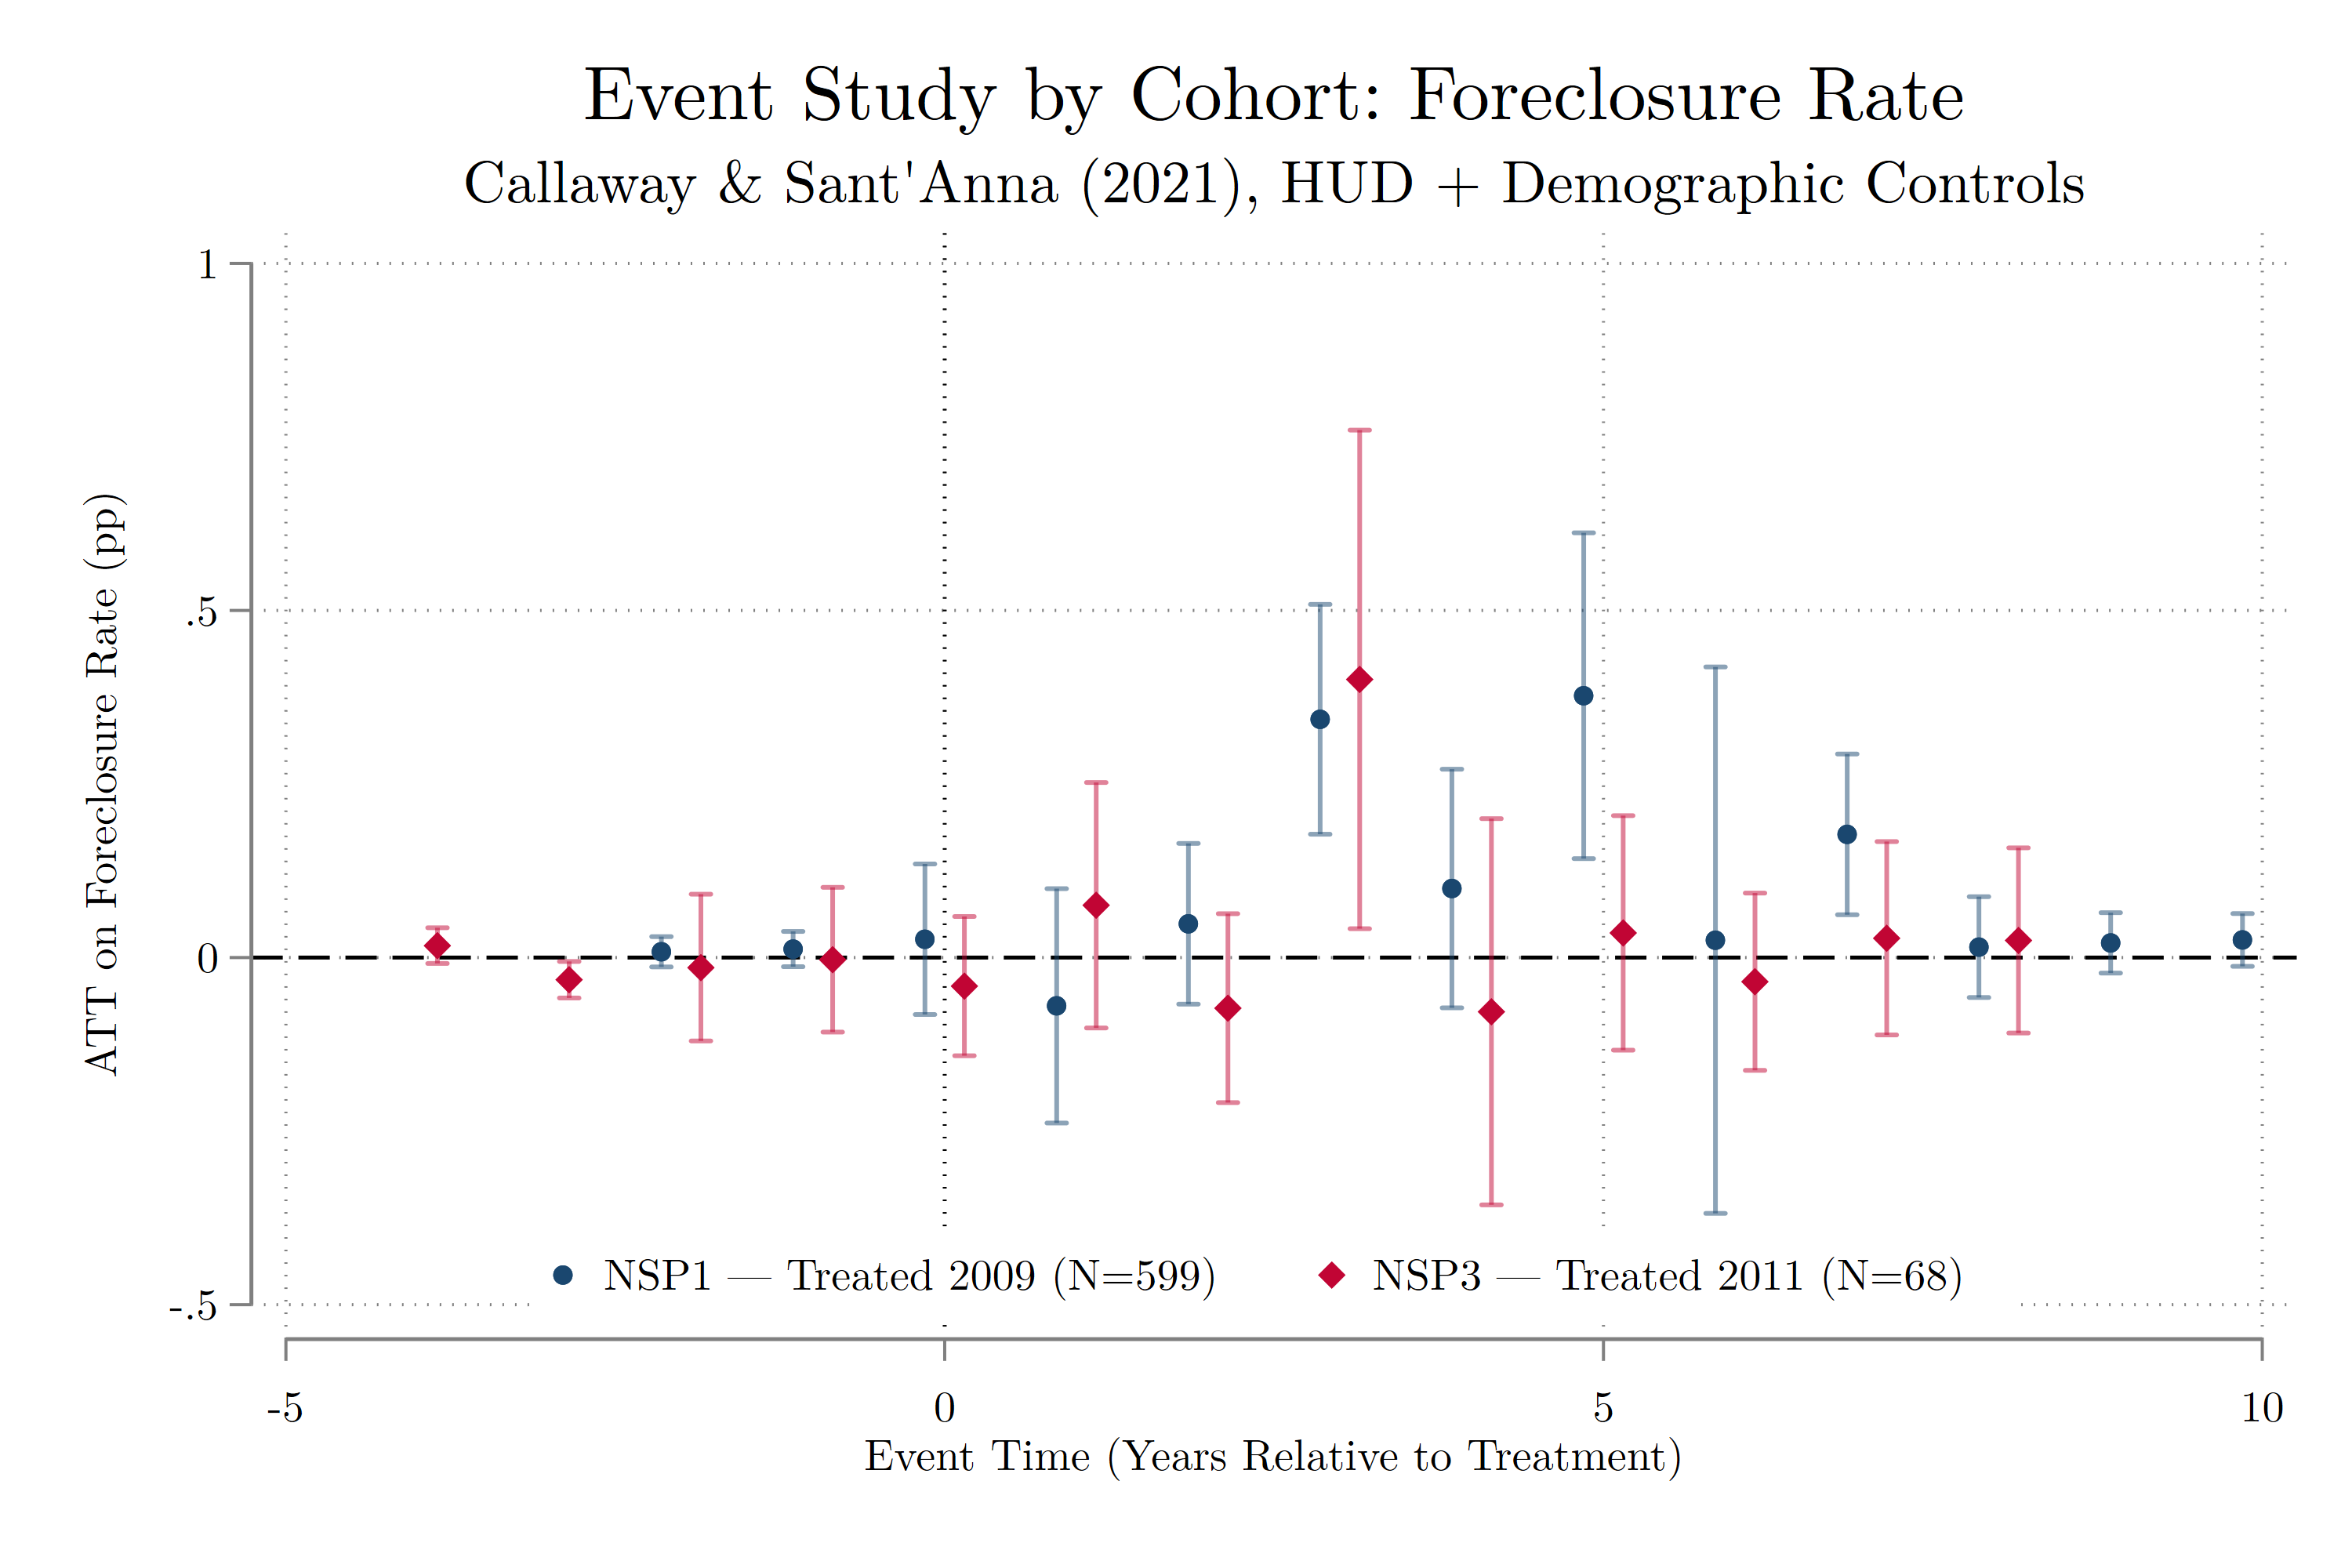
\includegraphics[width=0.85\textwidth]{cs_cohort_fore_event.png}
\caption{Cohort-Specific Event Study: Foreclosure Rate}
\label{fig:cohort_event_fore}
\end{figure}

\section{Aggregated Event Studies}
\label{app:aggregated}

Figures~\ref{fig:agg_event_sale} and \ref{fig:agg_event_fore} present the aggregated event study results pooling across both treatment cohorts.

\begin{figure}[H]
\centering
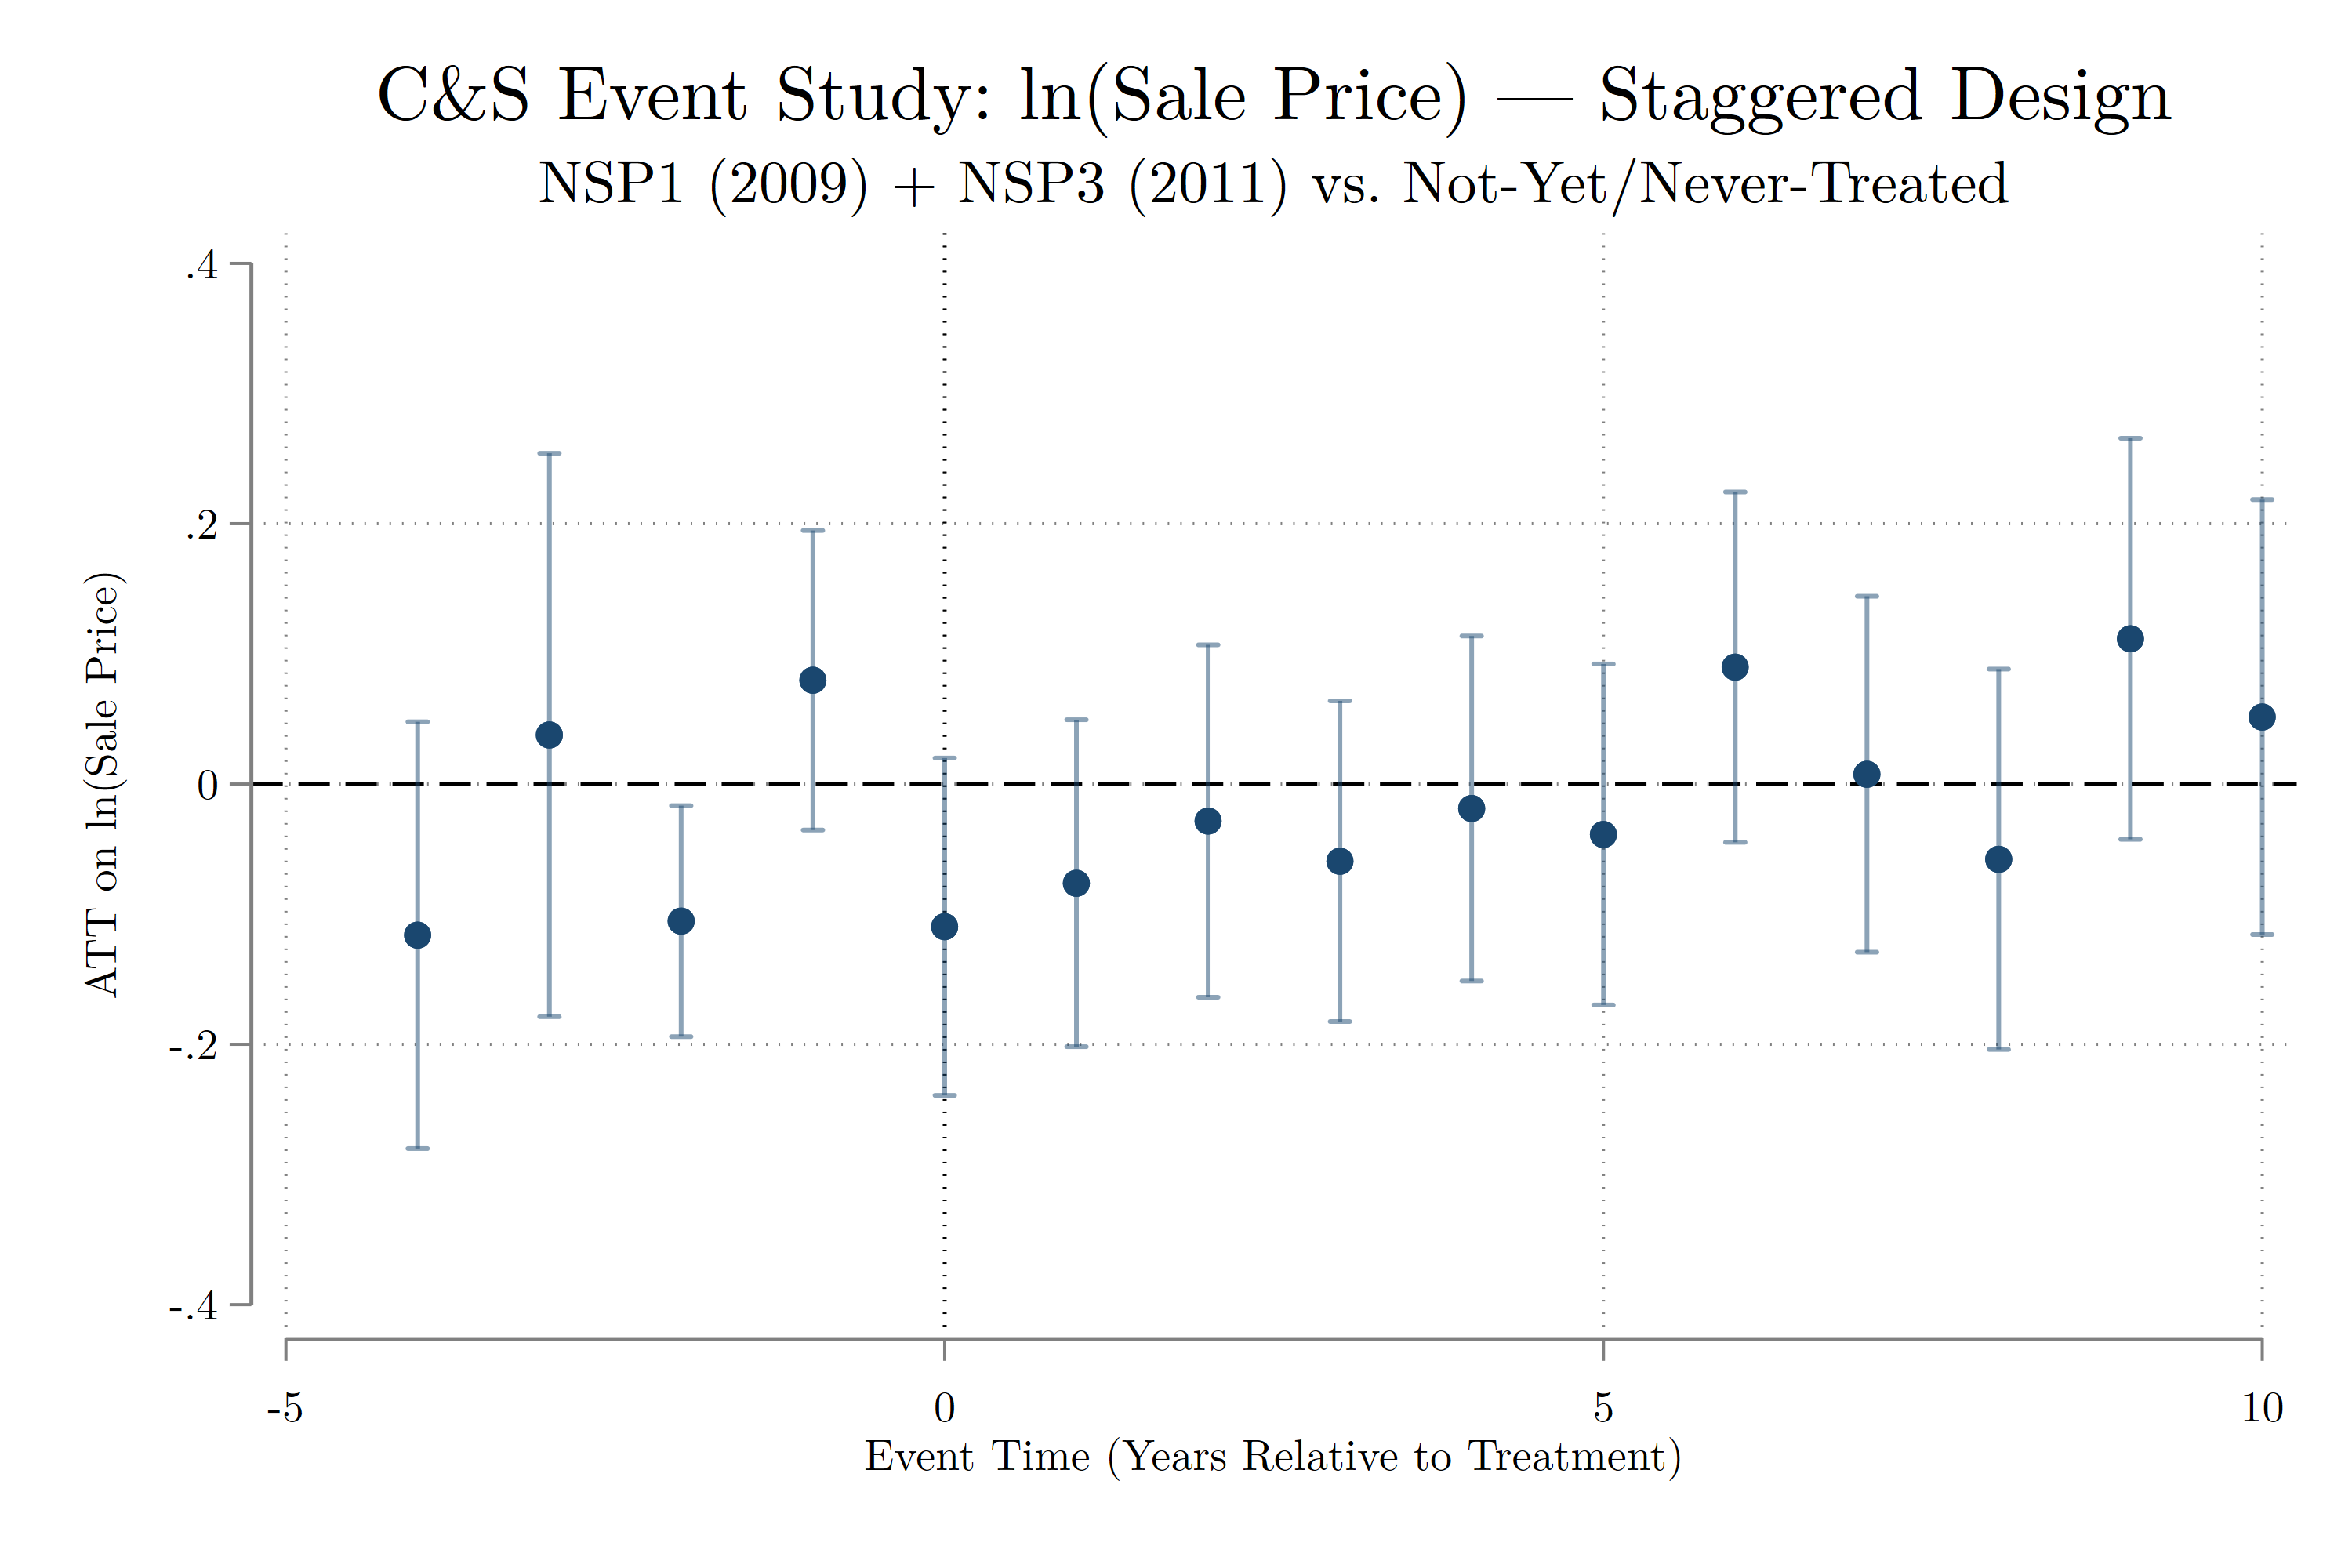
\includegraphics[width=0.85\textwidth]{cs_staggered_sale_event.png}
\caption{Aggregated Event Study: ln(Sale Price)}
\label{fig:agg_event_sale}
\end{figure}

\begin{figure}[H]
\centering
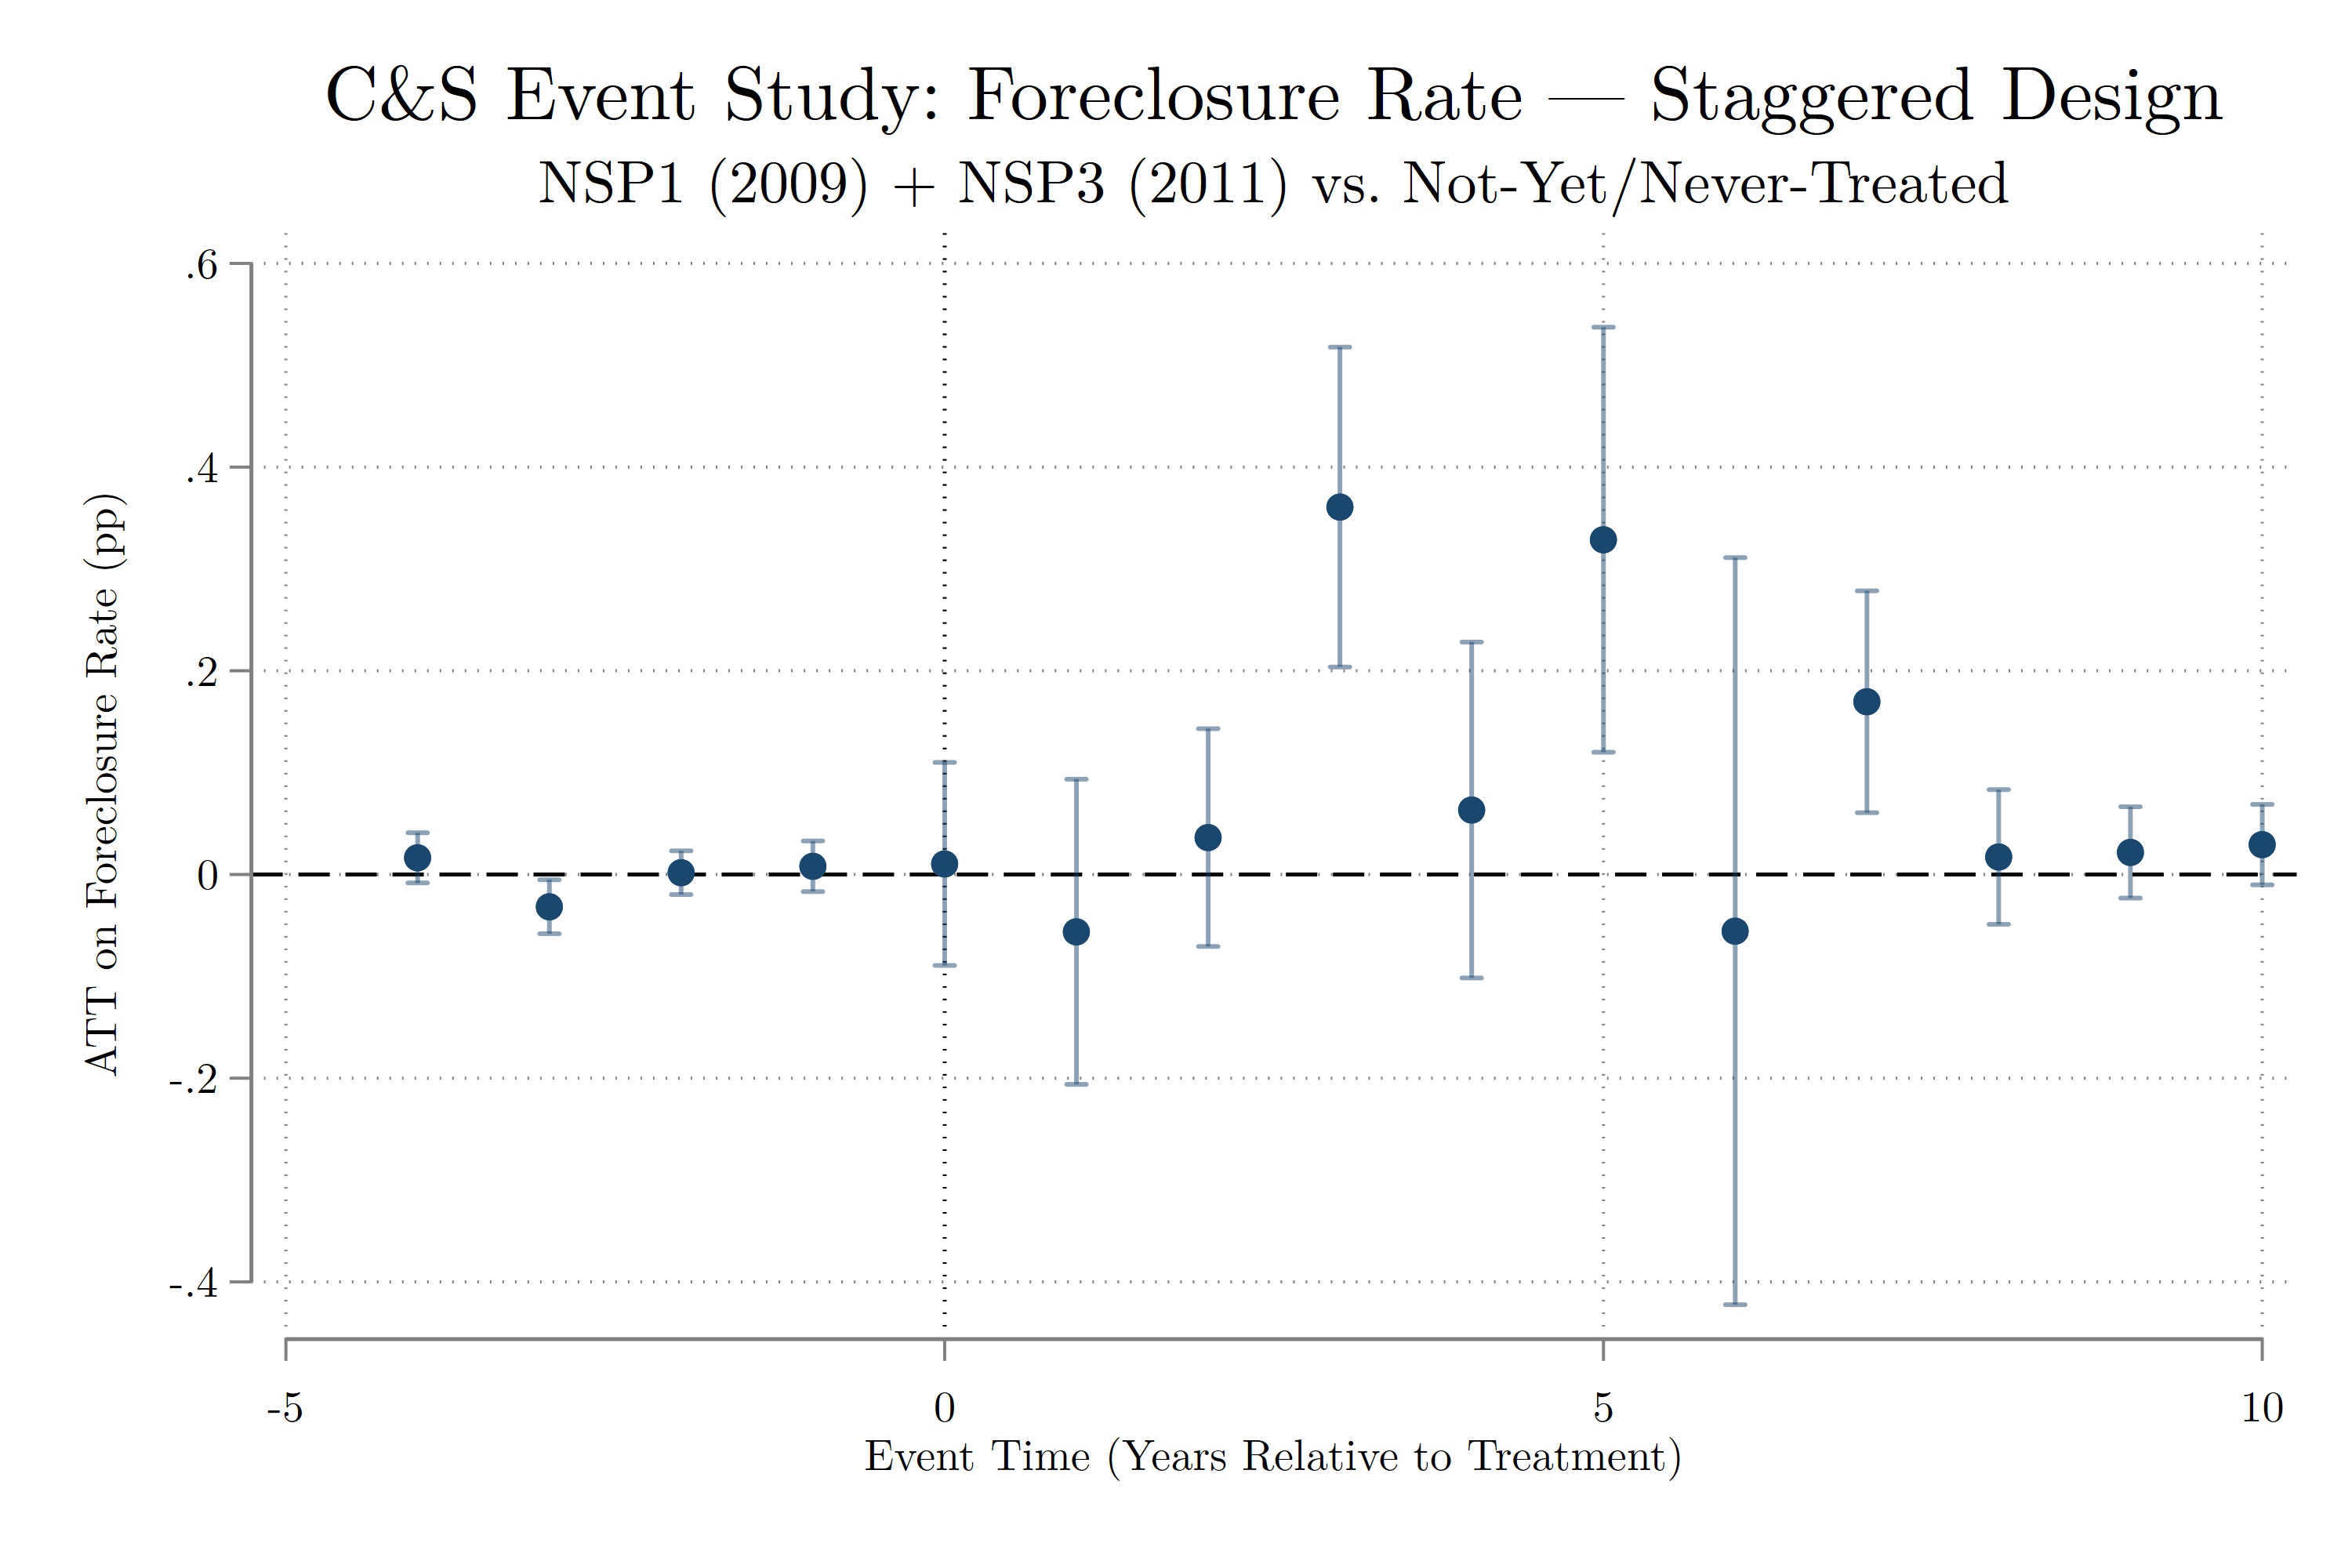
\includegraphics[width=0.85\textwidth]{cs_staggered_fore_event.png}
\caption{Aggregated Event Study: Foreclosure Rate}
\label{fig:agg_event_fore}
\end{figure}

\section{Sale Price Trends in Levels}
\label{app:levels}

Figure~\ref{fig:trends_levels} presents the sale price trends in levels (dollars), illustrating why the log transformation is preferred. The level trends show non-parallel pre-treatment paths due to the highly skewed distribution of sale prices in Detroit, while the log transformation (Figure~\ref{fig:trends_lprice}) produces substantially more parallel pre-trends.

\begin{figure}[H]
\centering
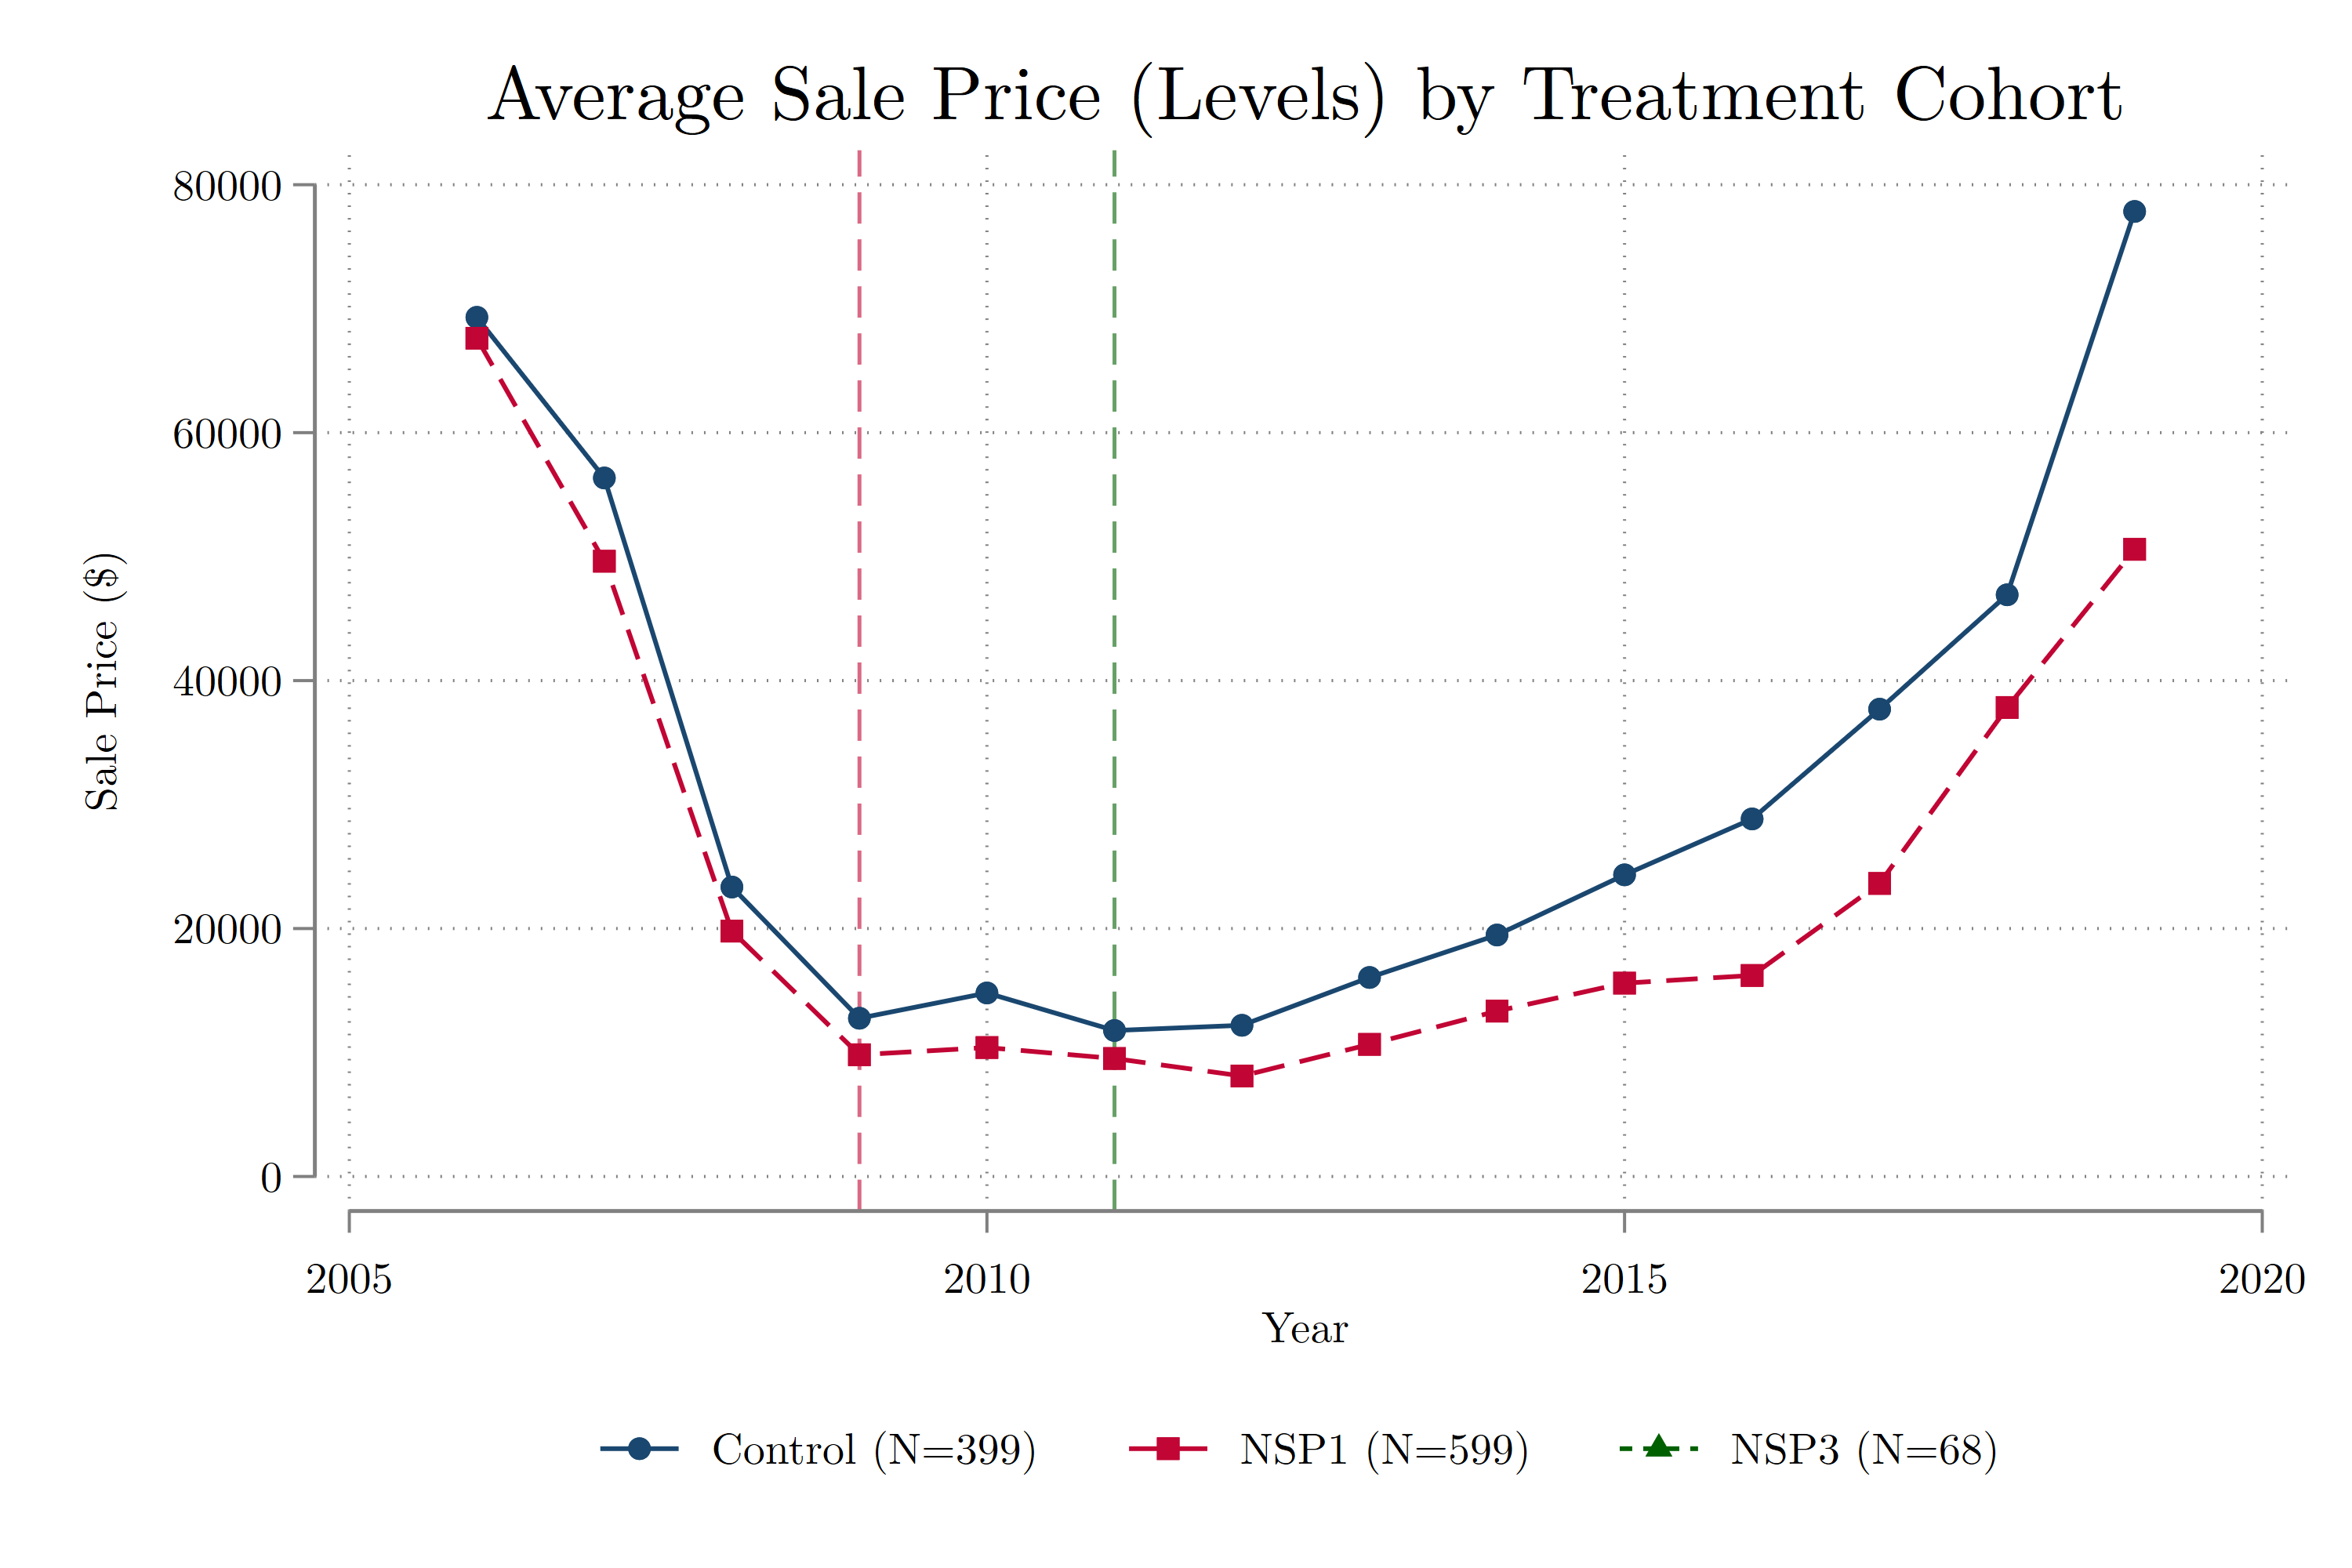
\includegraphics[width=0.85\textwidth]{pretrend_saleprice_staggered.png}
\caption{Descriptive Trends: Average Sale Price in Levels by Treatment Cohort}
\label{fig:trends_levels}
\end{figure}

\section{RDD Infeasibility}
\label{app:rdd}

A natural question is whether the HUD formula variables could be used to implement a regression discontinuity design. Figure~\ref{fig:rdd_foreclo} shows that the predicted foreclosure rate has a smooth, positive relationship with treatment probability, with no sharp discontinuity that would support an RDD approach. The HUD risk score is essentially constant across all Detroit block groups (mean $= 9.87$, with the 25th through 90th percentiles all equal to 10), reflecting the fact that the entire city qualified as highly distressed. NSP selection in Detroit was discretionary at the project level, driven by HUD data and local priorities, rather than by a formula with a clear cutoff.

\begin{figure}[H]
\centering
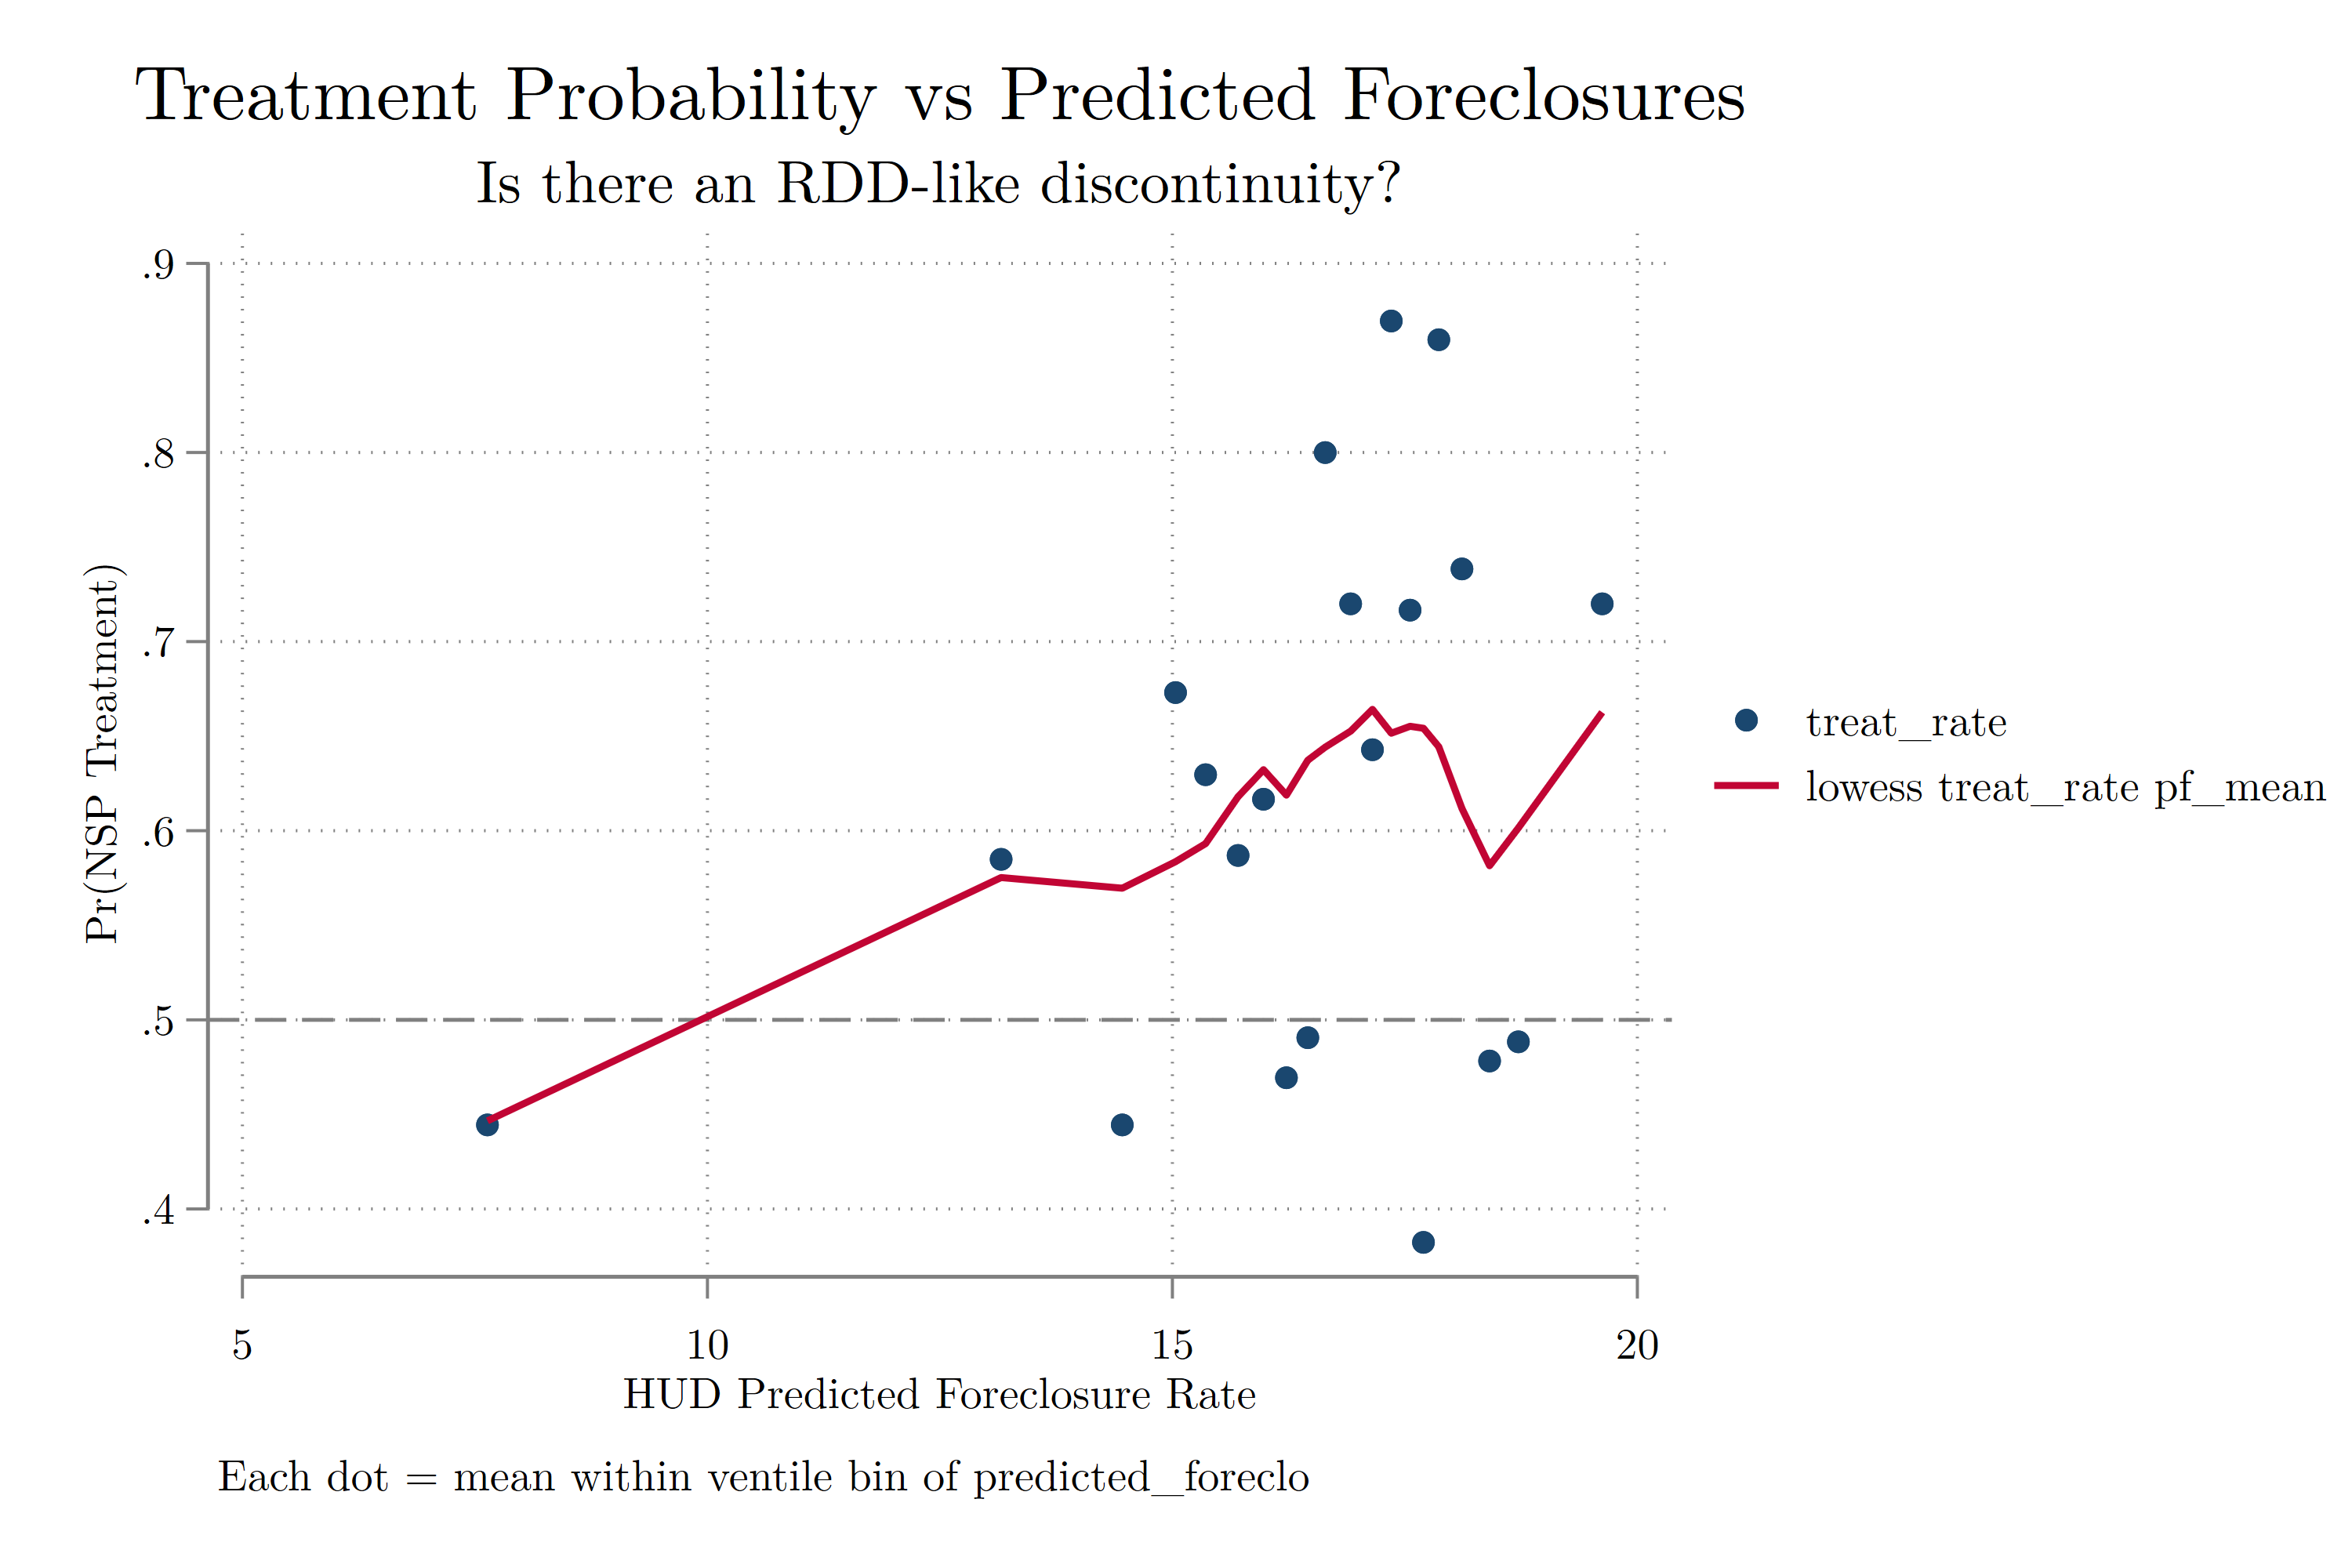
\includegraphics[width=0.85\textwidth]{rdd_check_predicted_foreclo.png}
\caption{Treatment Probability vs.\ Predicted Foreclosure Rate}
\label{fig:rdd_foreclo}
\end{figure}


\section{Variable Descriptions}
\label{app:variables}

\begin{table}[H]
\centering
\caption{Description of Variables Used in the Analysis}
\label{tab:variables}
\begin{threeparttable}
\small
\begin{tabularx}{\textwidth}{p{3.5cm}p{5cm}p{2cm}X}
\toprule
Variable & Description & Geographic Level & Source \\
\midrule
Sale Price & Average residential property sale price & Block group & ZTRAX (Zillow) \\
ln(Sale Price) & Natural log of average sale price & Block group & Authors' calculation \\
Foreclosure Rate & Foreclosures / total housing units & Block group & Data Driven Detroit \\
NSP1 & $=1$ if in NSP1 target zone & Block group & City of Detroit \\
NSP3 & $=1$ if in NSP3 target zone & Block group & City of Detroit \\
Predicted Foreclosure & HUD predicted foreclosure rate & Block group & HUD \\
Loan Rate & \% homes with subprime loans & Block group & HUD \\
Vacancy Rate & USPS residential vacancy rate & Block group & HUD \\
Risk Score & HUD composite risk score & Block group & HUD \\
\% Black & Percent African American & Block group & ACS \\
MHI & Median household income & Block group & ACS \\
Distance to CBD & Distance to Central Business District & Block group & GIS \\
Age & Mean age of properties & Block group & ZTRAX \\
Lot Size & Mean lot size (sq ft) & Block group & ZTRAX \\
\bottomrule
\end{tabularx}
\begin{tablenotes}[flushleft]
\footnotesize
\item \textit{Source:} Authors' compilation. Time-invariant variables based on 2009 data. Time-varying variables observed annually 2006--2019.
\end{tablenotes}
\end{threeparttable}
\end{table}


\end{document}
